%%% File encoding: UTF-8
%%% äöüÄÖÜß  <-- keine deutschen Umlaute hier? UTF-faehigen Editor verwenden!

\documentclass[bachelor,german]{hgbthesis}
% Zulässige Class Options: 
%   Typ der Arbeit: diplom, master (default), bachelor, praktikum 
%   Hauptsprache: german (default), english
%%%----------------------------------------------------------

\RequirePackage[utf8]{inputenc}		% Bei der Verw. von lualatex oder xelatex entfernen!

\graphicspath{{images/}}    % Abbildungsverzeichnis
\logofile{logo}				% Name des Logo-PDFs in images/ (\logofile{}, wenn kein Logo gewünscht)
\bibliography{literatur}  	% Name der Biblatex-Literaturdatei (.bib)

%%%----------------------------------------------------------
% Angaben für die Titelei (Titelseite, Erklärung etc.)
%%%----------------------------------------------------------

%%% Einträge für ALLE Arbeiten: -----------------------------
\title{Konzeption und prototypische Umsetzung einer webbasierten WYSIWYG-Anwendung zur Datenpflege}
\author{Benjamin\ Schuch}
\studiengang{Angewandte Informatik}
\studienort{Berlin}
\abgabedatum{2016}{08}{22}	% {YYYY}{MM}{DD}

%%% Zusätzlich für eine Bachelorarbeit: ---------------------
\nummer{533347}   % Stud-ID, z.B. 1310238045-A  
% (A = 1. Bachelorarbeit)
\semester{Sommersemester 2016} 
%\gegenstand{Einführung in die Tiefere Problematik 1} 
\betreuer{} % oder \betreuerin{..}

%%% Restriktive Lizenformel anstatt CC (nur für Typ master) -
%\strictlicense

%%%----------------------------------------------------------
\begin{document}
%%%----------------------------------------------------------

%%%----------------------------------------------------------
\frontmatter                    % Titelei (röm. Seitenzahlen)
%%%----------------------------------------------------------

\maketitle

\chapter*{Kurzfassung}

In der vorliegenden Arbeit wird die Entwicklung einer Verwaltungsplattform für die Pflege komplexer Datenstrukturen beschrieben. Dabei handelt es sich konkret um Filterdaten einer bereits bestehenden Software für die Bestimmung und Konfiguration von Druck- und Durchflussmessgeräten, die von der Yokogawa Deutschland GmbH hergestellt werden. Die entstehende Verwaltungsplattform wird durch eine Webanwendung realisiert und die dafür benötigte Kommunikation mit einem Server mittels eines Webservice umgesetzt.

Ein Schwerpunkt der Arbeit ist die Analyse bestehender Datenstrukturen und die darauf aufbauende Konzeption einer REST-konformen Schnittstelle. Die zu gestaltende Benutzeroberfläche realisiert dabei Konzepte der datengetriebenen Generierung von Steuerelementen auf Grundlage der gegebenen Datenbasis. Aufgrund der geteilten Datenbasis zwischen der bestehenden Konfigurationssoftware und der zu entwickelten Webanwendung werden außerdem \acf{WYSIWYG} Gestaltungskonzepte angewendet, um eine effiziente und robuste Datenpflege zu realisieren.


		
%\chapter*{Abstract}

\begin{english} %switch to English language rules
This should be a 1-page summary of my work in English language.
%und hier geht dann das Abstract weiter...
\end{english}


\tableofcontents
\addcontentsline{toc}{chapter}{Abbildungsverzeichnis}
\listoffigures
\addcontentsline{toc}{chapter}{Tabellenverzeichnis}
\listoftables
\addcontentsline{toc}{chapter}{Listingverzeichnis}
\lstlistoflistings

%\chapter{Vorwort} 	% engl. Preface
 % Optional. Ggf. weglassen
\chapter{Abkürzungsverzeichnis}
\begin{acronym}
  \acro{AJAX}{Asynchronous JavaScript and XML}
  \acro{CSS}{Cascading Style Sheets}
  \acro{DNS}{Domain Name System}
  \acro{DOM}{Document Object Model}
  \acro{EN}{Europäische Norm}
  \acro{ISO}{Internationale Organisation für Normung}
  \acro{HTTP}{Hypertext Transfer Protocol}
  \acro{HTTPS}{Hypertext Transfer Protocol Secure}
  \acro{IANA}{Internet Assigned Numbers Authority}
  \acro{IP}{Internetprotokoll}
  \acro{JSON}{JavaScript Object Notation}
  \acro{JWT}{JSON Web Token}
  \acro{MSSQL}{Microsoft SQL}
  \acro{MVC}{Model-View-Controller}
  \acro{NPM}{Node Package Manager}
  \acro{ORM}{Object-Relational Mapping}
  \acro{REST}{Representational State Transfer}
  \acro{RFC}{Request for Comments}
  \acro{ROA}{Resource-Oriented Architecture}
  \acro{SPA}{Single-Page-Anwendung}
  \acro{SSL}{Secure Socket Layers}
  \acro{TCP}{Transmission Control Protocol}
  \acro{TDS}{Tabular Data Stream}
  \acro{URI}{Uniform Resource Identifier}
  \acro{URL}{Uniform Resource Locator}
  \acro{WWW}{World Wide Web}
  \acro{WYSIWYG}{What You See Is What You Get}
  \acro{XML}{Extensible Markup Language}
\end{acronym}

%%%----------------------------------------------------------
\mainmatter          % Hauptteil (ab hier arab. Seitenzahlen)
%%%----------------------------------------------------------

\chapter{Einleitung}
\label{cha:Einleitung}

\section{Problemstellung}
\label{sec:Problemstellung}

Die Firma netbase GmbH aus Berlin betreut als Großkunden die Yokogawa Deutschland GmbH. Zu deren Hauptgeschäftsfeldern gehören die Herstellung und der Vertrieb von verteilten Prozessleitsystemen sowie von Druck- und Durchflussmessgeräten. Für die Verwaltung und Konfiguration dieser Geräte wurde von der netbase GmbH eine Individualsoftware mit der Bezeichnung FlowConfigurator entwickelt. Diese Software, ermöglicht es den Vertriebsmitarbeiter der Yokogawa Deutschland GmbH anhand von Kundenspezifikationen den geeigneten Sensor aus dem umfangreichen Produktbestand zu bestimmen und anschließend zu konfigurieren. Dabei findet ein vielschichtiges Filtersystem Anwendung, welches logisch abstrahiert in einer Datenbank organisiert ist. Die Filterdaten umfassen dabei sowohl gerätespezifische Merkmale, als auch Zuordnungen zu Sensoren und Produktkategorien, auf Grundlage derer die Sensorenauswahl eingeschränkt werden kann. Die Filtersteuerelemente in Form von Dropdown-Listen und Schaltern werden auf Grundlage dieser Datenbasis zur Laufzeit in der FlowConfigurator Software generiert und angeordnet. 

Die Anforderungen an die vorhandenen Filter können sich jedoch ändern oder müssen erweitert werden, wenn zum Beispiel neue Produkte eingeführt werden. Dies verursacht erhöhten Pflegeaufwand auf Seiten der netbase GmbH, da die Filter bisher nur direkt in der Datenbank angepasst und erweitert werden können. Durch die Entwicklung einer Verwaltungsoberfläche zur Pflege und Organisation der Filterdaten soll dieser Prozess in Zukunft effizienter und robuster gestaltet werden.

\newpage

\section{Zielsetzung}
\label{sec:Zielsetzung}

Ziel im Rahmen dieser Arbeit ist die prototypische Entwicklung einer Software zur Pflege von Filterdaten des FlowConfigurator. Diese Software soll als Webapplikation technisch getrennt von der FlowConfigurator Software realisiert werden. Die Datenbasis des FlowConfigurator wird dabei in Form einer \ac{MSSQL} Datenbank von der netbase GmbH bereitgestellt. Für die Realisierung des Projekts, gilt es die technischen und theoretischen Grundlagen zu erarbeiten. Ein Schwerpunkt ist die Analyse der vorliegenden Datenstruktur und die darauf aufbauende Funktionsweise des FlowConfigurator hinsichtlich Benutzerführung und Filterlogik. Da die Filterdaten nicht nur aus Merkmalen und Verknüpfungen bestehen, sondern zusätzlich auch Layout- und Typinformationen der zu generierenden Filtersteuerelemente beinhalten, ist es notwendig, neben Dateneingabemasken für Zuordnungen und Eigenschaften, auch Konzepte für die Anpassung der layoutspezifischen Daten zu entwickeln. Insbesondere ist hier die ebenfalls anpassbar zu machende Anordnung und Gruppierung der Filtersteuerelemente zu nennen. Aus diesem Grund soll die zu gestaltende Benutzeroberfläche auf dem \ac{WYSIWYG} Prinzip aufbauen und der des FlowConfigurator in Bezug auf Layout und Funktionsweise ähneln. Dies soll eine eingängliche und effektive Anpassung der Filterdaten, insbesondere der Anordnung der Filtersteuerelemente, ermöglichen. 

Wie bereits in Abschnitt \ref{sec:Problemstellung} angedeutet liegen die Filter als Datenrepräsentation eines komplexen und vielschichtigen Filtersystems vor. Deshalb ist es für die Spezifikation einer Schnittstelle notwendig, Abhängigkeiten auf Datenbankebene zu identifizieren und bedarfsabhängig zusammenzufassen.  Ebenso muss eine Homogenisierung der Daten in Betracht gezogen werden, um eine möglichst leichtgewichtige und einheitliche Schnittstelle zu schaffen. Diese Schnittstelle soll die Grundlage eines Webservice bilden, der vom Client konsumiert wird. Der Webservice soll außerdem vor Fremdzugriffen geschützt werden und deshalb ein rudimentäres Authentifizierungssystem implementieren.

Nach dem Bearbeiten der Filterdaten sollen diese durch einen Datenexport im FlowConfigurator wieder nutzbar gemacht werden. Das übergeordnete Ziel ist dabei sowohl der Erhalt der Datenintegrität als auch die Sicherstellung einer korrekten Funktionsweise der Sensorfilterung und Darstellung der Filtersteuerelemente hinsichtlich eines möglichen angepassten Layouts.

\newpage

\section{Aufbau der Arbeit}

Die Arbeit beginnt mit der Betrachtung von thematischen Grundlagen, die zum Verständnis der Arbeit beitragen. Eine intensive Betrachtung des \acf{REST} Architekturstils im Kontext einer \acf{ROA} bildet den Einstieg in diese Arbeit. Anschließend wird das Wissenschaftsgebiet Software-Ergonomie anhand des Schwerpunktes Grundsätze der Dialoggestaltung beleuchtet und in diesem Zusammenhang eine Übersicht über Evaluations- und Prüftechniken gegeben.

Das dritte Kapitel der Arbeit beinhaltet die Anforderungsanalyse. Hier werden Anwendungsfälle beschrieben, die von dem zu entwickelnden Prototyp abgedeckt werden und Anforderungen definiert. Des Weiteren findet eine Betrachtung und Vergleich von in Frage kommenden Technologien statt.

Gegenstand des vierten Kapitels ist zum einen die Beschreibung der gewählten Software-Architektur, als auch ein Entwurfskonzept der zu gestaltenden Benutzeroberfläche. Weiterhin werden Überlegungen zum Schnittstellenentwurf diskutiert und in diesem Zusammenhang das zugrunde liegende Datenmodell beschrieben.

Im fünften Kapitel wird auf Grundlage der vorher getätigten Analysen und Entwürfe die Implementierung des Prototyps beschrieben. Dabei wird auf die Besonderheiten der Umsetzung eingegangen und das Zusammenspiel der eingesetzten Technologien betrachtet. 

Das sechste Kapitel beinhaltet den Test des Prototyps. Die angewandte Testmethode wird mit Bezug auf den Versuchsaufbau beschrieben und das zu erwartende Ergebnis benannt. Eine Testauswertung stellt abschließend den Bezug zum tatsächlichen Testergebnis her.

Den Abschluss bildet eine Bewertung des entwickelten Prototyps, sowie eine Zusammenfassung zur Erweiterbarkeit und bestehenden Problemen der aktuellen Implementierung.
\chapter{Thematische Grundlagen}
\label{cha:Thematische Grundlagen}

In diesem Kapitel werden thematische Grundlagen beleuchtet, die zum Verständnis dieser Arbeit beitragen. In Abschnitt \ref{sec:ROA} wird das Architekturmuster \ac{ROA} anhand ausgewählter Aspekte erläutert. Dabei wird insbesondere Bezug auf die Einordnung von ROA im Kontext von \ac{REST} genommen. Abschließend wird in Abschnitt \ref{sec:software-ergonomie} Software-Ergonomie und deren Bedeutung für die Erstellung benutzerfreundlicher Oberflächen in der Softwareentwicklung behandelt. Es werden jeweils nur Grundlagen vermittelt und auf weiterführende Literatur verwiesen.

\section{Resource-Oriented Architecture (ROA)}
\label{sec:ROA}

\subsection{Definition und Einordnung im Kontext von REST}
\label{sec:ROA:Definition und Einordnung im Kontext von REST}

\acf{ROA} ist ein Architekturmuster der Informationstechnik aus dem Bereich der verteilten Systeme, um Dienste von IT-Systemen zu strukturieren und zu nutzen. Der Begriff Ressource ist dabei bezeichnend für ein zentrales Element dieses Architekturmusters. Als Ressource im Kontext von \ac{ROA} wird im Allgemeinen jede Komponente einer Anwendung bezeichnet, die verwendet oder adressiert werden muss. Ressourcen können dabei sowohl physische Objekte\footnote{Zum Beispiel Sensoren oder Temperatursonden.}, als auch abstrakte Datenobjekte beschreiben. \parencite[vgl.][2]{REST2010} Das Ansprechen dieser Ressourcen über ein Netzwerk definierte Roy Fielding in seiner Dissertation aus dem Jahr 2000 erstmals als \acf{REST}. Fielding fasst REST dabei als eine Reihe von Grundsätzen für die Gestaltung von netzwerkbasierten Software-Architekturen zusammen. Ziel der Anwendung dieser Grundsätze ist es den Netzwerkdurchsatz und die dabei entstehenden Latenzzeiten in einem verteilten System zu minimieren und gleichzeitig die Unabhängigkeit und damit einhergehende bessere Skalierbarkeit der einzelnen Komponenten zu fördern. \parencite[vgl.][35,76]{Fielding2000} Werden diese Grundsätze bei der Implementierung eines Webservices berücksichtigt spricht man auch von REST-konformen bzw. RESTful Webservices.

Es lässt sich erkennen, dass die Definition von \ac{REST} und \ac{ROA} aufgrund ihrer Ressourcenorientierung stark ineinandergreifen. Beide Begriffe werden deshalb oft auch synonym verwendet. Die synonyme Verwendung beider Begriffe ist aus akademischer Sicht aber nicht schlüssig. Denn während \ac{ROA} ein Architekturmuster beschreibt, definiert Fielding \ac{REST} als einen Architekturstil. Wo liegen also die Unterschiede zwischen einer Architektur und einem Architekturstil?

Eine Software-Architektur ist die Struktur einer Anwendung oder Computersystems, bestehend aus Software-Komponenten und deren nach außen sichtbaren Schnittstellen, sowie die Beziehung, die zwischen diesen Komponenten beschrieben werden kann \parencite[vgl.][21]{Bass2003}. Ein Architekturstil umfasst hingegen eine Menge von Architekturen deren Eigenschaften sich hinsichtlich der typischen strukturellen Organisation ihrer Komponenten und deren Kommunikation untereinander gleichen \parencite[vgl.][20]{Shaw1996}.

Anhand dieser Definitionen lassen sich \ac{ROA} und \ac{REST} nun klar voneinander abgrenzen. \ac{REST} beschreibt demnach nur eine Menge von Entwurfskriterien auf Grundlage derer Software-Architekturen realisiert werden können. Erfüllt eine Architektur alle diese Entwurfskriterien, spricht man von einer \ac{ROA}. Das bedeutet im Umkehrschluss aber auch, dass es andere Software-Architekturen geben kann, die das Konzept \ac{REST} ganz oder auch nur teilweise implementieren.

\subsection{Grundsätze des REST-Architekturstils}
\label{sec:ROA:Grundsätze des REST-Architekturstils}

Die Grundsätze die Fielding für \ac{REST} in \citetitle[77\psqq]{Fielding2000} definiert, sind nicht das Ergebnis rein theoretischer Überlegungen, sondern das Ergebnis der Analyse der Funktionsweise des \ac{WWW}. Die Zusammenfassung dieser Ergebnisse als Grundsätze eines neuen Architekturstils sind seitdem Bestandteil verschiedener Architekturmuster in der Software-Entwicklung und Gegenstand dieses Abschnitts.

\subsubsection{Client-Server}

Der erste Grundsatz beschreibt die Trennung zwischen Server und Client. In diesem Grundsatz findet sich das Prinzip \emph{Separation of Concerns}\footnote{Siehe \hyperlink{https://effectivesoftwaredesign.com/2012/02/05/separation-of-concerns/}{https://effectivesoftwaredesign.com/2012/02/05/separation-of-concerns/}.} wieder, welches die Trennung von Zuständigkeitsbereichen propagiert. Dieser Ansatz verbessert die Skalierbarkeit und Portabilität, da die einzelnen Komponenten auf Server- und Clientseite einfach gehalten und getrennt voneinander entwickelt werden können.

\subsubsection{Zustandslosigkeit}
\label{sec:ROA:Zustandslosigkeit}

Dieser Grundsatz bezieht sich auf die zustandslose Kommunikation in einer Client-Server-Interaktion. Das bedeutet, dass in einer Anfrage an den Server alle benötigten Informationen zur Bearbeitung der Anfrage enthalten sein müssen. Die Verwaltung von Sitzungen liegt nach Fielding ausschließlich beim Client. Da keine Daten zwischen verschiedenen Anfragen gespeichert werden müssen, wird dadurch die Zuverlässigkeit der Komponenten erhöht. Außerdem ist es einfacher, den Status des Systems nach einem Auftritt von Fehlern wiederherzustellen. Ein Nachteil ist jedoch die erhöhte Netzwerklast aufgrund des Sendens von wiederkehrenden Informationen in aufeinanderfolgenden Anfragen gleichen Typs.

\subsubsection{Caching}

Um die Netzwerklast zu verringern, beschreibt Fielding ein Verfahren zum clientseitigen Zwischenspeichern von Daten. Jede Kommunikation zwischen Client und Server soll dabei auf ihre Cachefähigkeit gekennzeichnet werden. Ist eine Anfrage cachefähig, wird bei wiederholtem Aufruf die Antwort des Servers im Client aus einem Zwischenspeicher geladen. \parencite[vgl.][79\psqq]{Fielding2000} Dieses Konzept kann, wenn davon auszugehen ist das sich Daten zwischen verschiedenen Anfragen über einen längeren Zeitraum hinweg nicht ändern, die Performance verbessern und die Netzwerklast damit senken. Ist allerdings davon auszugehen, dass sich die Daten häufig ändern, kann die Implementierung eines Cache dazu führen, dass der Client veraltete Daten aus dem Zwischenspeicher bereitstellt.

\subsubsection{Einheitliche Schnittstelle}
\label{sec:ROA:Einheitliche Schnittstelle}

Ein Kernkonzept des REST-Architekturstils ist die Etablierung einer einheitlichen und allgemeinen Schnittstelle, über die Komponenten kommunizieren. Dadurch werden Implementierungen von den bereitgestellten Services entkoppelt. Dies vereinfacht die Gesamtarchitektur und fördert zusätzlich die Skalierbarkeit. \parencite[vgl.][81\psq]{Fielding2000} Allerdings muss eine einheitliche Schnittstelle nicht in jedem Fall den spezifischen Anforderungen einer Applikation genügen, was negativen Einfluss auf die Effektivität der Implementierung haben kann. Da \ac{REST} von den Bedürfnissen des \ac{WWW} abgeleitet wurde, eignet sich die REST-Schnittstelle besonders für groß angelegte Applikationen, in denen Effektivität zugunsten der Einfachheit der Schnittstellenimplementierung niedriger priorisiert werden kann. Für die Implementierung einer einheitlichen Schnittstelle definierte Fielding \parencite[82]{Fielding2000} weiterhin vier Grundsätze:
\newpage
\begin{itemize}
\item Bestimmung von Ressourcen
\item Manipulation von Ressourcen über Repräsentationen
\item Selbstbeschreibende Nachrichten
\item Hypermedia als Engine des Application State
\end{itemize}
Diese Grundsätze werden in Abschnitt \ref{sec:ROA:Bestandteile des REST-Architekturstils} näher betrachtet.

\subsubsection{Geschichtetes System}

Ein aus verschiedenen Schichten bestehendes System erlaubt eine klare Trennung von Zuständigkeiten. Jede Schicht hat nur Kenntnis über die jeweiligen Schichten, mit denen sie kommunizieren muss. Damit wird die Gesamtkomplexität des Systems durch natürliche Schranken in der Architektur verringert. \parencite[vgl.][82\psqq]{Fielding2000} Zum Beispiel können damit Proxies oder Gateways als Mittel zur Lastenverteilung als Kommunikationsschicht zwischen Server und Client etabliert werden. Auch eine Auslagerung von bestehenden Codestrukturen in eigene Schichten kann sinnvoll sein, wenn es zum Beispiel notwendig wird, die Funktionalität von Legacy-Code zu erhalten, währenddessen der Service in einer anderen Schicht weiterentwickelt wird. Je mehr Schichten in das System eingeführt werden, desto höher ist allerdings auch die Verzögerung in der Verarbeitung der Daten.

\subsubsection{Code-On-Demand}

Der letzte Grundsatz des REST-Architekturstils ist Code-On-Demand. Damit beschreibt Fielding die Möglichkeit des Clients Programmcode herunterzuladen und auszuführen, welcher in Applets oder Skripten zur Verfügung gestellt wird. Der Client kann dadurch zur Laufzeit dynamisch erweitert werden, was die Komplexität und den Umfang verringern kann. \parencite[vgl.][84\psq]{Fielding2000}

\subsection{Bestandteile des REST-Architekturstils
}
\label{sec:ROA:Bestandteile des REST-Architekturstils}

\subsubsection{Datenelement}
\label{sec:ROA:Datenelement}

Datenelemente im Sinne von \ac{REST} sind Repräsentationen von Informationen, die zwischen Komponenten (über ein Netzwerk) transportiert werden. Das Format der Informationen wird dabei dynamisch durch die Art der Ressource und den Anforderungen des Clients aus einer Menge von Standartdatentypen bestimmt. In Tabelle \ref{tab:dataelements} sind die Datenelemente des REST-Architekturstils dargestellt, die nachfolgend erläutert werden. 

\begin{table}[H]
\centering
\def\rr{\rightskip=0pt plus1em \spaceskip=.3333em \xspaceskip=.5em\relax}
\setlength{\tabcolsep}{1ex}
\def\arraystretch{1.20}
\setlength{\tabcolsep}{1ex}
\small
\begin{tabular}{|p{0.4\textwidth}|p{0.4\textwidth}|}
\hline
   \multicolumn{1}{|c}{\emph{Datenelement}} &
   \multicolumn{1}{|c|}{\emph{Beispiele}} \\
\hline\hline
   {\rr Resource} &
   Ziel einer Hypertext Referenz
   \\
\hline
  {\rr Resource Identifier} &
  URL, URN
  \\
\hline
  {\rr Representation} &
  HTML-Dokument, JPG-Datei
  \\
\hline
  {\rr Representation Metadata} &
  Medientyp, Änderungsdatum
  \\
\hline
  {\rr Resource Metadata} &
  source link, alternates, vary
  \\
\hline
  {\rr Control Data} &
  if-modified-since, cache-control
  \\
\hline
\end{tabular}
\caption{REST Datenelemente}
\label{tab:dataelements}
\end{table}

Eine \emph{Ressource} ist die Kernabstraktion einer Information des REST-Architekturstils. Eine Ressource wird nach Fielding als eine Abbildungsfunktion beschrieben, die zu einer bestimmten Zeit eine Menge von Werten abbildet. Diese Werte können \emph{Repräsentationen} von Ressourcen sowie Ressourcenbezeichner sein. \emph{Ressourcenbezeichner} werden verwendet, um Ressourcen eindeutig zu identifizieren bzw. zu adressieren. Auf einer Ressource werden von Komponenten Aktionen ausgeführt, die als Ergebnis Repräsentationen von Ressourcen erzeugen. Diese Repräsentationen werden an andere Komponenten übertragen und bestehen dabei aus Informationen aus der Ressource selbst, sowie \emph{Metadaten}, die diese Informationen beschreiben. \emph{Kontrolldaten} werden zusätzlich übertragen, um zum einen den Zweck der Nachricht zu beschreiben, als auch Zusatzfunktionen, wie zum Beispiel Caching-Verhalten, zu steuern. \parencite[vgl.][88\psqq]{Fielding2000}

\subsubsection{Konnektoren}

Verschiedene Typen von Konnektoren werden verwendet, um den Zugriff auf Ressourcen und die Übertragung ihrer Repräsentationen zu kapseln. Die Implementierung einer Komponente wird durch die Einführung von Konnektoren, die man auch als abstrakte Schnittstellen verstehen kann, von der Kommunikationslogik getrennt. In Abschnitt \ref{sec:ROA:Einheitliche Schnittstelle} wurde die zustandslose Kommunikation als ein Grundsatz des REST-Architekturstils beschrieben. Aufgrund dieser Zustandslosigkeit können Konnektoren Anfragen parallel abarbeiten, da kein Zusammenhang zwischen einzelnen Anfragen besteht. \parencite[vgl.][93]{Fielding2000} Die in diesem Abschnitt eingangs erwähnten verschiedenen Konnektortypen werden in Tabelle \ref{tab:connectors} dargestellt und nachfolgend erläutert.

\begin{table}[H]
\centering
\def\rr{\rightskip=0pt plus1em \spaceskip=.3333em \xspaceskip=.5em\relax}
\setlength{\tabcolsep}{1ex}
\def\arraystretch{1.20}
\setlength{\tabcolsep}{1ex}
\small
\begin{tabular}{|p{0.4\textwidth}|p{0.4\textwidth}|}
\hline
   \multicolumn{1}{|c}{\emph{Konnektor}} &
   \multicolumn{1}{|c|}{\emph{Beispiele}} \\
\hline\hline
   {\rr Client} &
   libwww, libwww-perl
   \\
\hline
  {\rr Server} &
  libwww, Apache API, NSAPI
  \\
\hline
  {\rr Cache} &
  browser cache
  \\
\hline
  {\rr Resolver} &
  adns (DNS-Lookup Bibliothek)
  \\
\hline
  {\rr Tunnel} &
  SOCKS, SSL
  \\
\hline
\end{tabular}
\caption{REST Konnektoren}
\label{tab:connectors}
\end{table} 

Client- und Serverkonnektor sind die beiden wichtigsten Konnektortypen. Während der \emph{Clientkonnektor} stets eine Kommunikation mit dem Senden einer Anfrage einleitet, reagiert der \emph{Serverkonnektor} nur auf diese Anfragen und verschickt nach der Bearbeitung eine Antwort. 
Auf den Schnittstellen von Client- und Serverkonnektor befinden sich \emph{Cachekonnektoren}. Diese haben die Aufgabe über die Cachefähigkeit einer Nachricht zu entscheiden und bei Bedarf ein Abbild einer Nachricht zu speichern. Dies kann auf Client- und auf Serverseite geschehen, um die Netzwerklast zu verringern bzw. um den Prozess der Erstellung der Antwortnachricht nicht mehrfach ausführen zu müssen. 
Der \emph{Resolvekonnektor} übersetzt den Ressourcenbezeichner in eine Netzwerkadresse, um die für den physikalischen Netzwerkzugriff benötigten Daten zu erhalten.
Schließlich übernimmt der \emph{Tunnelkonnektor} die Aufgabe Informationen über Systemgrenzen (z.B. Firewalls) hinweg zu transportieren. \parencite[vgl.][93\psq]{Fielding2000}

\subsubsection{Komponenten}

Komponenten werden nach Fielding anhand ihrer Rolle im Kontext der Gesamtanwendung zusammengefasst. Nachfolgend werden die in Tabelle \ref{tab:components} dargestellten Komponenten betrachtet.

\begin{table}[H]
\centering
\def\rr{\rightskip=0pt plus1em \spaceskip=.3333em \xspaceskip=.5em\relax}
\setlength{\tabcolsep}{1ex}
\def\arraystretch{1.20}
\setlength{\tabcolsep}{1ex}
\small
\begin{tabular}{|p{0.4\textwidth}|p{0.4\textwidth}|}
\hline
   \multicolumn{1}{|c}{\emph{Komponente}} &
   \multicolumn{1}{|c|}{\emph{Beispiele}} \\
\hline\hline
   {\rr Origin Server} &
   Apache httpd, NGINX, Microsoft IIS
   \\
\hline
  {\rr Gateway} &
  Squid, CGI
  \\
\hline
  {\rr Proxy} &
  Netscape Proxy, CERN Proxy
  \\
\hline
  {\rr User Agent} &
  Mozilla, Chrome, Lynx
  \\
\hline
\end{tabular}
\caption{REST Komponenten}
\label{tab:components}
\end{table}

Ein \emph{User Agent} verwendet einen Clientkonnektor, um eine Anfrage zu initiieren und ist gleichzeitig der Empfänger der Antworten dieser Anfrage. User Agents können zum Beispiel Webbrowser sein, die nach dem Aufruf einer Ressource ein Dokument anzeigen. Der \emph{Origin Server} nutzt einen Serverkonnektor, um den Namespace für eine angefragte Ressource zu verwalten. Dabei stellt er eine in Abschnitt \ref{sec:ROA:Einheitliche Schnittstelle} beschriebene generische Schnittstelle zum Zugriff auf Ressourcen bereit. Die Details der Implementierung eines Servers und seiner Komponenten sind dabei hinter der Schnittstelle versteckt und für andere Komponenten des Systems nicht sichtbar. Gateway- und Proxy-Komponenten agieren als Zwischenstellen im Kontext des Nachrichtenverlaufs zwischen Client und Server. Dabei wird ein \emph{Proxy} in der Regel von einem Client angefragt, wenn es zum Beispiel notwendig wird, Schnittstellen anderer Services zu kapseln oder den Service abzusichern. Ein \emph{Gateway} wird auch als Reverse Proxy bezeichnet und erfüllt dieselbe Funktion wie ein Proxy, wird aber durch das Netzwerk oder den Server gesteuert. \parencite[vgl.][97]{Fielding2000}

\subsection{Prinzipien einer Ressource-Oriented Architecture
}
\label{sec:ROA:Prinzipien einer Ressource-Oriented Architecture}

In Abschnitt \ref{sec:ROA:Definition und Einordnung im Kontext von REST} wird \ac{REST} als eine Sammlung von Prinzipien definiert, die zusammengefasst als Architekturstil, ein wesentliches Mittel zum Entwurf und zur Implementierung einer \ac{ROA} darstellen. \ac{REST} setzt dabei auf die Nutzung des \ac{HTTP} und seiner Möglichkeiten. REST-konforme Webservices müssen dabei aber nicht zwingend auf \ac{HTTP} basieren; derzeit ist es aber das einzige existierende und praktisch angewandte Protokoll. Maßgeblich beeinflusst wurde diese Technologieempfehlung durch Fielding, der gleichzeitig auch einer der Hauptautoren der HTTP-Spezifikation ist. Für eine \acl{ROA} wird deshalb als Technologiebasis \acs{URI}, \acs{HTTP} und \acs{XML} empfohlen. \parencite[vgl.][80]{Ruby2007} Nachfolgend werden anhand der in Abschnitt \ref{sec:ROA:Grundsätze des REST-Architekturstils} beschriebenen REST-Grundsätze, die Prinzipien einer ROA auf Basis der eben genannten Technologien beispielhaft beschrieben und auf mögliche Probleme eingegangen.

\subsubsection{Adressierbarkeit}

In Abschnitt \ref{sec:ROA:Datenelement} wird eine Ressource als eine Abbildungsfunktion beschrieben. Im Kontext einer \ac{ROA} kann diese zum Beispiel ein Algorithmus, eine Datenbankoperation oder Ähnliches sein, die über ein Netzwerk zugänglich ist. Die Adresse und der Name einer Ressource kann durch einen \ac{URI} eindeutig global identifiziert werden. Nachfolgend wird der Aufbau einer \ac{URI} nach dem \ac{RFC} Standard 3986, verfasst von \citeauthor{BernersLee1998}, erläutert. 

\begin{center}
\setlength{\fboxrule}{0.2mm}
\setlength{\fboxsep}{2mm}
\fbox{
\begin{minipage}{0.9\textwidth}
Protokoll://Host:Port/Pfad?Querystring/\#fragment
\end{minipage}}
\end{center}

Das \emph{Protokoll} gibt an, welches Kommunikationsprotokoll zur Übertragung von Nachrichten genutzt werden soll. In \ac{ROA} sind das meistens \ac{HTTP} oder \ac{HTTPS}.
Der \emph{Host} ist der \ac{DNS} Name oder die \ac{IP} Adresse einer adressierten Ressource. Die Angabe des \emph{Ports} erlaubt die Ansteuerung eines optionalen \ac{TCP} Ports. Der \emph{Pfad} beschreibt eine konkrete Ressource auf dem Server. Zusätzlich können über einen \emph{Querystring} weitere Informationen als Wertepaare an den Server übertragen werden. Ein \emph{Fragment} wird schließlich dazu verwendet eine bestimmte Stelle in einem Dokument anzuzeigen.
Eine \ac{URI} sollte nach \citeauthor[83]{Ruby2007} so aufgebaut sein, dass die Bedeutung der referenzierten Ressource daraus hervorgeht. Eine Ressource kann dabei auch von mehreren \ac{URI} adressiert werden.

\subsubsection{Einheitliche Schnittstelle}
\label{sec:ROA:Einheitliche Schnittstelle}

die HTTP-Spezifikation umfasst bereits eine Menge von Methoden, mit denen sich Ressourcen manipulieren lassen. In Tabelle \ref{tab:httpmethods} sind diese Methoden aufgelistet und beschrieben. Es gibt noch weitere HTTP-Methoden, wie TRACE oder CONNECT, diese spielen aber im Kontext eines RESTful-Webservice meist keine Rolle und werden deswegen nicht näher erläutert.

\begin{table}[H]
\centering
\def\rr{\rightskip=0pt plus1em \spaceskip=.3333em \xspaceskip=.5em\relax}
\setlength{\tabcolsep}{1ex}
\def\arraystretch{1.20}
\setlength{\tabcolsep}{1ex}
\small
\begin{tabular}{|p{0.2\textwidth}|p{0.6\textwidth}|}
\hline
   \multicolumn{1}{|c}{\emph{Methode}} &
   \multicolumn{1}{|c|}{\emph{Beschreibung}} \\
\hline\hline
   {\rr GET} &
Wird verwendet um die Information einer Ressource abzufragen (read-only).
   \\
\hline
  {\rr PUT} &
Fügt eine Repräsentation einer Ressource hinzu oder aktualisiert sie.
  \\
\hline
  {\rr DELETE} &
Löscht eine Repräsentation einer Ressource
  \\
\hline
  {\rr POST} &
Hinzufügen von Repräsentationen einer 	Ressource.
  \\
\hline
  {\rr HEAD} &
Wird verwendet um Metadaten einer Ressource 	abzufragen
  \\
\hline
  {\rr OPTIONS} &
Wird verwendet um Informationen über die Kommunikationsoptionen einer Ressource abzufragen.
  \\
\hline
\end{tabular}
\caption{HTTP-Methoden und ihre Bedeutung im Kontext eines RESTful-Webservice}
\label{tab:httpmethods}
\end{table}

Um eine Repräsentation einer Ressource abzufragen oder zu löschen, sendet der Client nur eine GET- oder DELETE-Anforderung an die \ac{URI} der Ressource. Im Falle einer GET-Anforderung, antwortet der Server mit einer Repräsentation der Ressource im HTTP-Body. Für eine DELETE-Anforderung kann der Inhalt des HTTP-Body eine Statusmeldung enthalten oder auch leer bleiben. Um eine Ressource zu erstellen oder zu aktualisieren, wird in der Regel eine PUT-Anforderung gesendet. Der HTTP-Body enthält dabei die neue oder aktualisierte Repräsentation einer Ressource. POST wird verwendet, wenn eine Ressource erstellt werden soll, deren \ac{URI} vorher nicht bekannt ist. Dabei wird ebenfalls die zu erstellende Repräsentation der Ressource im HTTP-Body verschickt. Anzumerken ist, dass in der Fachwelt immer wieder unterschiedlich über die Funktionsweise von POST und PUT diskutiert wird. In diesem Abschnitt bezieht sich der Autor dieser Arbeit auf \cite[97\psq]{Ruby2007}.

Das Datenformat für die Übertragung der Daten im HTTP-Body hängt in der Regel vom Service ab. Weit verbreitet ist \ac{XML}, dass aber zunehmend durch \ac{JSON} verdrängt wird. \ac{JSON} als Datenformat eignet sich besonders gut, wenn die Client-Komponenten einer \ac{ROA} mit Javascript realisiert werden, da sich JSON Nachrichten direkt in Javascript-Objekte übertragen lassen.

\subsubsection{Zustandslosigkeit}

In Abschnitt \ref{sec:ROA:Zustandslosigkeit} wurde Zustandslosigkeit bereits als ein Grundsatz des REST-Architekturstils dargestellt. Übertragen auf eine \ac{ROA} bedeutet Zustandslosigkeit, dass jede HTTP-Anfrage unabhängig und getrennt von allen vorherigen und nachfolgenden Anfragen erfolgt. Das bedeutet, dass immer alle Informationen die notwendig sind, um die Anfrage zu bearbeiten mitgeschickt werden müssen.

Bei einer \ac{ROA} wird zwischen zwei Zuständen unterschieden: Dem \emph{Application State}, der den Zustand des Clients bezeichnet, und dem \emph{Resource State}, den Zustand des Servers. Dabei ist der Application State für jeden Client unterschiedlich, wohingegen der Resource State für alle Clients gleich ist. Dieser Sachverhalt liegt darin begründet, dass ein Client in der Regel von mehreren Benutzern aufgerufen werden kann. Jeder Benutzer hat dabei seine ganz eigene Umgebung, in der er den Client nutzt, und definiert damit auch seinen eigenen Application State. Jeder Benutzer greift über den Client aber auf denselben Server zu. Der Resource State ist deshalb für alle Clients gleich. \parencite[vgl.][90\psq]{Ruby2007} 

Um echte Zustandslosigkeit zu erreichen, darf der Server nie Teile des Application States speichern und umgekehrt darf ein Application State nie Annahmen über den Resource State machen. Dieser Ansatz führt vor allem zu Problemen, wenn man den Zugriff auf eine Ressource auf einen bestimmten Nutzerkreis einschränken möchte (siehe Abschnitt \ref{sec:ROA:Sicherheit}).

\subsubsection{Repräsentationen}

In Abschnitt \ref{sec:ROA:Datenelement} wurden Repräsentationen als Datenelemente des REST-Architekturstils eingeführt. Eine Ressource erzeugt bei ihrem Aufruf über eine \ac{URI}, jeweils Repräsentationen ihres derzeitigen Zustands. Typischerweise sind in einer \ac{ROA} Ressourcen selbst Implementierungen, die auf Datenquellen zugreifen. Das ist zum Beispiel der Fall, wenn eine Ressource mit einer Datenbank verknüpft ist. Ressourcen müssen aber nicht zwangsweise abstrakte Datenobjekte beschreiben, sondern können, wie in Abschnitt \ref{sec:ROA:Definition und Einordnung im Kontext von REST} angedeutet, auch physische Objekte sein. Das können zum Beispiel Temperatursonden sein, die nicht einfach als abstraktes Datenobjekt beschrieben werden können. Die Repräsentation von physischen Ressourcen sind deshalb Metadaten, die Zustände oder Eigenschaften des physischen Objekts beschreiben. \parencite[vgl.][91]{Ruby2007}.

Zusätzlich ist es in einer \ac{ROA} oft notwendig, dass abhängig von der Anfrage des Clients, verschiedene Arten von Repräsentationen erzeugt werden müssen. Als Beispiel sind hier Ressourcen zu nennen, deren Daten in verschiedenen Sprachen vorliegen. Eine Ressource entscheidet in diesem Anwendungsfall anhand von Metadaten, die der Client beispielsweise im HTTP-Header mitsendet, welche Repräsentation der sprachsensitiven Inhalte erstellt werden müssen. Dieses Verhalten kann insbesondere zu Problemen führen, wenn der Client nicht weiß, welche Sprachen zur Verfügung stehen (da dies über die \ac{URI} erst einmal nicht ersichtlich ist) oder keine Angaben darüber macht, welche Sprache ausgeliefert werden soll. Die Ressource kann in diesem Fall nur Standardannahmen über die gewünschte Repräsentation machen. \citeauthor{Ruby2007} empfehlen daher, dass ein Client seine Anfragen immer so präzise wie möglich formulieren und nie auf Standardverhalten der Ressourcen vertrauen sollte. Das kann in einer komplexen \ac{ROA} Umgebung aber zu einer erhöhten Netzwerklast führen, da zusätzlich zum einfachen Aufruf einer \ac{URI} auch immer entsprechende Metadaten zur Steuerung der Ressourcen mitgeschickt werden müssen. \parencite[vgl.][94]{Ruby2007}

\subsection{Sicherheit}
\label{sec:ROA:Sicherheit}

Zur Absicherung von Ressourcen vor unautorisierten Zugriff stellt die HTTP-Spezifikation bereits eigene Mechanismen zur Verfügung. Bei HTTP und damit im Kontext dieses Abschnitts auch bei RESTful Webservices, findet die Verschlüsselung von Nachrichten typischerweise auf Transportebene auf Basis des \ac{SSL} statt. Authentifizierung und Autorisierung kann entweder durch Basic-Authentication, Digest-Authentication oder Token-Authentication erfolgen. Außerdem ist es zusätzlich möglich, Ressourcen per Rechtevergabe (ähnlich wie bei einem Dateisystem) abzusichern. So kann eine Ressource beispielsweise read-only gestaltet werden, indem sie nur für GET und HEAD implementiert wird. \parencite[vgl.][311\psq]{Ruby2007}

Auf Basis des \ac{RFC} 7519 Standards wird in diesem Abschnitt eine Möglichkeit der Token-basierten Authentifizierung näher beleuchtet.

\subsubsection{Authentifizierung nach \ac{RFC} 7519}

\ac{RFC} 7519 ist ein offener Standard, der eine Token-basierte Authentifizierung mithilfe eines \ac{JWT} beschreibt. Bei einer auf Tokens basierten Authentifizierung sendet der Client eine Anfrage an den Server mit den Benutzerdaten als Teile des HTTP-Body. Als Antwort bekommt der Client einen als \mbox{Base64} kodierten Token, der mit einem privaten Schlüssel erstellt und signiert wird. Die eindeutige Signatur stellt sicher, dass der Token im Nachhinein nicht manipuliert werden kann. Bei jeder weiteren Anfrage muss der Client nun diesen Token als Query-String oder im \ac{HTTP} Authorization-Header mitschicken. Der Token wird immer bei jeder Anfrage mit Hilfe des privaten Schlüssels validiert und gewährt entsprechend Zugriff auf die angefragte Ressource. In Bezug auf \ac{REST} ergibt sich damit ein wesentlicher Vorteil: Alle Informationen, die für die Validierung notwendig sind, sind in einem \ac{JWT}-Token enthalten, was die Zustandslosigkeit einer REST konformen Architektur fördert. \parencite[vgl.][13]{RFC7519} Ein \ac{JWT}-Token besteht aus drei Teilen: Dem Header, dem Payload und der Signatur. In Abbildung \ref{prog:jwtstructure} wird dieser Aufbau beispielhaft dargestellt und nachfolgend beschrieben.

\begin{figure}[H]
\begin{GenericCode}[numbers=none]
Header
{
    "alg": "HS256",
    "typ": "JWT"
},
Payload
{
    "iss": "authservice",
    "sub": "92d0312b-26b9-4887-a338-7b00fb3c5eab",
    "exp": 1431061608,
    "iat": 1390234181,
    "aud": ["http://example.de],
    "name": "John Doe",
    "role":	"Admin"
}
Signature 
{
	HS256
    (
      base64UrlEncode(header) + "." + 
      base64UrlEncode(payload), 
      secret
    )
}
\end{GenericCode}
\caption{Beispielhafter Aufbau eines \acf{JWT}}
\label{prog:jwtstructure}
\end{figure}

\paragraph{Header} Im Header befinden sich eine Reihe von Metadaten, die das Token selbst und dessen Funktionsweise beschreiben. Im Header muss mindestens das genutzte Hashverfahren und der Typ des Tokens angegeben werden. Das Hashverfahren wird für die Erstellung der Signatur genutzt und muss vom Server unterstützt werden.

\paragraph{Payload} Der Payload beinhaltet Informationen, die vom Server für die Authentifizierung des Benutzers benötigt werden. Claims werden als JSON-Objekt angegeben, wobei die Bezeichner der Wertepaare innerhalb eines Claims eindeutig sein müssen. Es wird zwischen drei verschiedenen Arten von Claims unterschieden.

\paragraph{Registered Claims} Die registrierten Claims sind formal Teil jedes \ac{JWT}-Token und sind im \ac{IANA} Register für \ac{JWT}-Token eingetragen und definiert. In \citetitle[8]{RFC7519} wird lediglich eine Empfehlung gegeben, welche Claims mindestens angegeben werden sollten. Die Inhalte dieser Claims sind applikationsabhängig, werden aber in der Regel unbedingt benötigt um ein Token zu validieren. Nachfolgend werden in Tabelle \ref{tab:claims} diese Claims beschrieben.

\begin{table}[H]
\centering
\def\rr{\rightskip=0pt plus1em \spaceskip=.3333em \xspaceskip=.5em\relax}
\setlength{\tabcolsep}{1ex}
\def\arraystretch{1.20}
\setlength{\tabcolsep}{1ex}
\small
\begin{tabular}{|p{0.3\textwidth}|p{0.5\textwidth}|}
\hline
   \multicolumn{1}{|c}{\emph{Claim}} &
   \multicolumn{1}{|c|}{\emph{Beschreibung}} \\
\hline\hline
   {\rr iss (Issuer)} &
   Der Aussteller des Tokens.
   \\
\hline
  {\rr sub (Subject)} &
Das Subjekt welche durch das gesamte Claim-Set beschrieben wird. Dies kann zum Beispiel eine Benutzer-ID sein.
  \\
\hline
  {\rr aud (Audience)} &
Der vorgesehene Empfänger des Tokens. Es können mehrere Empfänger durch ein Array angegeben werden.
  \\
\hline
  {\rr exp (Expiration Time)} &
Das Zeitintervall, für das ein Token gültig ist.
  \\
\hline
  {\rr iat (Issued At)} &
Die genaue Zeit, zu der das Token ausgestellt wurde.
  \\
\hline
  {\rr jti (JWT ID)} &
Der eindeutiger Bezeichner eines Tokens.
  \\
\hline
\end{tabular}
\caption{Empfohlene Claims für ein \acf{JWT} nach \ac{RFC} 7519}
\label{tab:claims}
\end{table}


\paragraph{Public Claims} Public Claims können selbst definiert werden. Es muss jedoch sichergestellt werden, das keine Namenskonflikte auftreten. Es wird daher empfohlen aus bereits im \ac{IANA} Register eingetragenen Claims zu wählen. Public Claims sind oft zusätzliche Angaben über den Benutzer, für den der Token ausgestellt wurde. Das können zum Beispiel Name, E-Mail-Adresse oder die Rolle des Benutzers innerhalb der Applikation sein. Alle Public Claims liegen, wie die Registered Claims, nicht kodiert vor und sind damit öffentlich. Sie dürfen deshalb keine sicherheitskritischen Informationen, wie etwa ein Passwort oder Ähnliches, enthalten.

\paragraph{Private Claims} Private Claims sind in der Regel Claims, die nur innerhalb eines bestimmten Applikationskontext relevant sind und unterliegen keinerlei Namenseinschränkungen.

\paragraph{Signature} Die Signatur des Tokens setzt sich aus den in Base64 konvertierten Header und Payloads eines \ac{JWT}-Tokens zusammen. Die entstehenden Zeichenketten werden durch einen Punkt getrennt und anschließend, wie in Abbildung \ref{prog:jwtstructure} aufgezeigt, mit einem privaten Schlüssel und dem angegeben Hashverfahren verschlüsselt.

\subsection{Zusammenfassung}

Die Prinzipien, die Fielding für \ac{REST} definierte, haben Einfluss auf viele Entwicklungen in der Software-Entwicklung genommen und sind heutzutage populärer denn je. Große Konzerne wie etwa Google und Amazon stellen ihre Webservices REST konform zur Verfügung und machen diese damit einfacher nutzbar. Die Beliebtheit lässt sich durch die verschiedenen Vorzüge erklären, die ein Ressourcen-orientierter Ansatz mit sich bringt:
\begin{itemize} 
\item Die einheitliche und generische Schnittstelle sichert ein erwartbares Verhalten beim Zugriff auf Ressourcen zu.
\item Gute Skalierbarkeit durch die Möglichkeit des Cachings und der Verwendung von Proxys und Gateways.
\item Die Möglichkeit der Absicherung durch eine Firewall schützt vor missbräuchlichen Zugriffen.
\item Die lose, flexible Kopplung von Komponenten begünstigt die Skalierbarkeit und Effektivität in der Entwicklung zusätzlich.
\item Die Unabhängigkeit von komplexen Protokollen erleichtert den Zugang und verringert die Komplexität der Anwendung.
\end{itemize}
Nicht zuletzt diese Vorteile machen \ac{ROA} als \glqq{}die REST-basierte Architektur\grqq{} populär. Vor allem im Bereich der Webentwicklung sind die Synergien offensichtlich und bekommen nicht zuletzt durch immer populärer werdende Javascript-Frameworks, wie zum Beispiel AngularJS oder EmberJS, zusätzlichen Aufwind. Die Tatsache das REST kein offizieller Standard ist, lässt bei der Anwendung seiner Prinzipien auf das Architekturmuster \ac{ROA} allerdings Interpretationsspielraum für einige der von Fielding beschriebene Grundsätze zu und kann dabei zu Verunsicherungen in der Frage führen \emph{\glqq{}Ist eine Architektur oder ein Webservice wirklich REST-konform?\grqq{}}. Die in den vorangegangenen Abschnitten erläuterten Vorgehensweisen zur Gestaltung einer \ac{ROA} können keine eindeutige Antwort auf diese Frage geben. Sie basieren auf Analysen und Interpretationen weniger Autoren - es gibt noch viele weitere Interpretationen, die in bestimmten Punkten abweichen können und in der Fachwelt diskutiert werden.

% -----------------------------------------------------
%\section{Scaffolding}
%\label{sec:scaffolding}
%
%\subsection{Definition und Methoden}
%
%Scaffolding beschreibt im Kontext der Software-Entwicklung einen Ansatz Quellcode automatisch zu generieren, um wiederkehrende Programmieraufgaben effizienter zu gestalten. Um %Scaffolding als Prozess zu verstehen ist es notwendig den Begriff eines Codegenerators zu spezifizeren. 
%Ein Programmgenerator ist ein Programm, das andere Programme erzeugt \parencite[vgl.][1]{Smaragdakis2004}. Diese Definition ist sehr unspezifisch und lässt noch keine Vorstellung über %den Zweck und Nutzen eines Codegenerators zu. Um diesen Sachverhalt besser zu verstehen hilft es typische Anwendungsgebiete von Codegeneratoren zu betrachten.
%
%
%\subsection{Methoden}
%
%\subsection{Auswirkungen auf den Entwicklungsprozess}
%
%\subsection{Zusammenfassung}
% -----------------------------------------------------

\section{Software-Ergonomie}
\label{sec:software-ergonomie}

\subsection{Definition und Einordnung}
\label{sec:software-ergonomie:Definition und Einordnung}

Um Software-Ergonomie zu definieren und einzuordnen, ist es zu Beginn notwendig, Ergonomie allgemein als ein Teilgebiet zu betrachten. Das Wort Ergonomie setzt sich aus den griechischen Worten \emph{ergon} (Werk, Arbeit) und \emph{nomos} (Regel, Gesetz) zusammen. Ergonomie beschreibt die Wissenschaft über die Gesetzmäßigkeit der menschlichen Arbeit und beschäftigt sich vornehmlich mit der Untersuchung von Prozessabläufen beim Einsatz beliebiger Produkte. Als Ziel dieser Untersuchungen steht die Optimierung der Gebrauchstauglichkeit (Usability) einer Mensch-Maschinen-Schnittstelle. Die Anwendung ergonomischer Grundsätze haben dabei eine Anpassung der Arbeitsbedingungen an den Menschen zur Folge, indem sie intuitive Bedienung fördern. Sie erhöhen Rentabilität menschlicher Arbeit, begrenzen Gefährdungen und steigern die Zufriedenheit des Anwenders. \parencite[vgl.][1\psq]{Wandmacher1993} Denn während ein schickes Design beim Anwender meist nur für temporäre Begeisterung sorgt, soll eine ergonomische Gestaltung den Benutzer auch über einen längeren Zeitraum motivieren mit einem Produkt zu arbeiten. 

Aufgrund des heutigen Stellenwertes in der Software-Entwicklung hat sich die Software-Ergonomie als ein eigenständiges Wissenschaftsgebiet entwickelt, welches sich insbesondere mit der Optimierung von Benutzerschnittstellen und Benutzeroberflächen beschäftigt. Eine Benutzerschnittstelle umfasst dabei diejenigen Komponenten und Aspekte eines Mensch-Computer-Systems, mit denen die Benutzer begrifflich oder über ihre Sinne und Motorik in Berührung kommen \parencite[vgl.][3\psqq]{Moran1981}. Das umfassende Themengebiet berührt dabei Aspekte der Beteiligung von Benutzern an der Software-Entwicklung, allgemeine Richtlinien und Normen, technische und organisatorische Rahmenbedingungen, Qualitätssicherung sowie den Einfluss der Software-Ergonomie auf wirtschaftliche Aspekte. Um diese Aspekte abzudecken, müssen viele verschiedene Disziplinen der Wissenschaft angewendet werden. Der umfangreiche internationale Standard EN ISO 9241 besteht aus insgesamt 17 Teilen, die alle Aspekte ergonomischer Softwaregestaltung beleuchten. Herauszuheben im Kontext dieser Arbeit ist die Norm EN ISO 9241-110 mit dem Titel \citetitle{ISO9241-110}, die in Abschnitt \ref{sec:ERG:Gestaltungsgrundsätze nach EN ISO 9241-110} beleuchtet wird.

\subsection{Gestaltungsgrundsätze nach EN ISO 9241-110}
\label{sec:ERG:Gestaltungsgrundsätze nach EN ISO 9241-110}

Der Teil 110 der DIN EN ISO 9241 beschreibt eine Reihe von Grundsätzen für die Gestaltung und Bewertung einer Schnittstelle zwischen Benutzer und System (Dialoggestaltung). Die Norm ersetzt seit 2006 den früheren Teil 10. Gleichzeitig wurde der Anwendungsbereich erweitert, die Norm gilt nun nicht mehr nur für Software und Bildschirmarbeit, sondern allgemein für alle \glqq{}interaktiven Systeme\grqq{}. Gerade bei den oft recht komplexen Aufgaben einer modernen Webapplikation mit unterschiedlichen Bedien- und Eingabemöglichkeiten wird die Benutzbarkeit zu einem immer wichtigeren Erfolgsfaktor. Die Norm EN ISO 9241-110 beschreibt sieben zentrale Grundsätze der Dialoggestaltung, die nachfolgend erläutert werden.

\subsubsection{Aufgabenangemessenheit}

Dieser Grundsatz stützt sich auf die Merkmale Effektivität und Effizienz. Effektivität ist dabei die Genauigkeit und Vollständigkeit, mit der der Nutzer seine Aufgabe lösen kann. Effizienz hingegen ist der eingesetzte Aufwand im Verhältnis zur Genauigkeit und Vollständigkeit, mit der eine Aufgabe vom Benutzer erledigt wird. Ein interaktives System sollte den Benutzer unterstützen, seine Aufgabe zu erledigen. Dabei sollten alle Tätigkeiten, die nicht direkt mit dem Erreichen dieses Ziels zusammenhängen vom System erledigt werden. Der Nutzer sollte sich nur mit der Bearbeitung von sogenannten externen Aufgaben, die sich direkt aus der Arbeitsaufgabe ergeben, beschäftigen müssen. Die Erledigung seiner Aufgabe sollte mit so wenig Arbeitsschritten wie möglich realisierbar und die Oberfläche der Zielgruppe der Benutzer entsprechen. \parencite[vgl.][169\psqq]{Herczeg2009}

\subsubsection{Steuerbarkeit}

Steuerbarkeit sagt aus, dass der Benutzer das System kontrollieren können muss. Geschwindigkeit und Arbeitsreihenfolge muss nach den Bedürfnissen und Fertigkeiten des Benutzers anpassbar sein. Um verschiedenen Benutzergruppen gerecht zu werden, sollte es ebenfalls möglich sein, die Ein- und Ausgabe kontextabhängig anzupassen. Man unterscheidet zwischen system- und benutzergesteuerten Dialogen. Eine gesteuerte Nutzerführung ist dabei vor allem in komplexen Systemen häufig nicht zu vermeiden. Es wird jedoch wenn möglich eine Mischform empfohlen, bei der eine Sequenz vom Benutzer gestartet wird und diese dann in ihrer Geschwindigkeit regulierbar ist.\parencite[vgl.][179\psqq]{Herczeg2009} Bei sicherheitskritischen Systemen kann jedoch nicht immer auf eine rein systemgesteuerte Dialogkontrolle verzichtet werden.

\subsubsection{Erwartungskonformität}

Durch einen aus dem Alltag vieler nicht mehr wegzudenkenden Umgang mit Computersystemen entstehen Erfahrungen, aus denen sich Erwartungen bei der Benutzung ähnlicher Systeme ergeben. \citeauthor{Herczeg2009} definiert Erwartungskonformität als ein Maß dafür, wie gut ein System diese Erwartungen erfüllt. Systeme, die den Erwartungen ihrer Benutzer gerecht werden, erleichtern die Bildung eines geeigneten mentalen Modells des Systems. Grundsätzlich sollte ein System in sich konsistent sein und dabei vorhandenen Konventionen folgen. Neben der Gestaltung von Dialogen spielt aber auch die Performance eines Systems eine wesentliche Rolle. Wenn die Reaktionszeiten, aufgrund von schlecht optimierten Netzwerkoperationen oder Algorithmen, zu sehr vom gewohnten Verhalten abweicht, kann das beim Benutzer zu Verunsicherungen führen. Vorhersehbar unerwartetes Verhalten sollte deshalb mit Hilfe von Nachrichten, Fortschrittsanzeigen oder ähnlichem mit dem Benutzer kommuniziert werden. \parencite[vgl.][175\psqq]{Herczeg2009}

\subsubsection{Selbstbeschreibungsfähigkeit}

Es muss für einen Benutzer jederzeit ersichtlich sein, wo genau er sich gerade innerhalb einer Anwendung befindet. Dieses Systemverständnis sollte ohne besondere Hinweise oder Einführungen durch eine fundierte Oberflächengestaltung gewährleistet sein. Vor allem bei komplexen Anwendungen ist es aber zusätzlich notwendig verständliche und möglichst kontextabhängige Hilfen anzubieten, um den Benutzer zu ermöglichen den derzeitigen Status der Anwendung zu erkennen. \parencite[vgl.][172\psqq]{Herczeg2009}

\subsubsection{Individualisierbarkeit}

Die Gestaltung eines Systems kann nie den individuellen Vorstellungen jedes einzelnen Benutzers gerecht werden. Um diesen Makel zu kompensieren, sollten wichtige Teile des Layouts individualisierbar sein. Der Bedarf und die Möglichkeiten der Individualisierbarkeit hängen dabei von dem zu entwickelnden System ab. Um ein Beispiel zu nennen: Häufig wird der Benutzer nach dem Anmeldevorgang an einer Webapplikation auf ein Dashboard weitergeleitet. Solch ein Dashboard gibt meist einen Überblick über wichtige Informationen des Systems. Die Wichtigkeit solcher Informationen wird von jedem Benutzer unterschiedlich wahrgenommen und sollte deswegen hinsichtlich der Anordnung und dem Inhalt anpassbar sein. \parencite[vgl.][186\psqq]{Herczeg2009} 

Das bedeutet jedoch keinesfalls, dass die Möglichkeit der Individualisierung gute Standardoberflächen ersetzt. Insbesondere ist zu vermeiden, dass Individualisierung zu Beeinträchtigungen in der Bedienung führen, etwa weil bestimmte Funktionen oder Inhalte durch Möglichkeiten der Individualisierung nicht mehr erreichbar oder versteckt sind. Ein weiterer Aspekt ist der erhöhte Pflegeaufwand und kompliziertere Support, den ein stark individualisierbares System nach sich zieht. Es sollte deshalb auch im Sinne der Aufgabenangemessenheit immer eine wohldurchdachte Abwägung zwischen individualisierbaren Oberflächen und Standardoberflächen erfolgen. \parencite[vgl.][189]{Herczeg2009}

\subsubsection{Lernförderlichkeit}

Eine Anwendung soll den Benutzer beim Einstieg und dem Erlernen der Bedienung eines Systems unterstützen und
anleiten. Außerdem ist es notwendig, diese Lernmechanismen nicht nur unmittelbar nach dem Einstieg anzubieten, sondern ebenfalls die Möglichkeit zu schaffen erfahrenen Benutzern eine Wiederauffrischung des Gelernten anzubieten. Lernförderlichkeit ist daher ein Aspekt, der bereits bei der Konzeption des Systems bedacht werden muss. Jedes System wird für einen bestimmten Zweck entwickelt und ist für den Benutzer ein Mittel zur Erfüllung seiner Aufgaben. Das bedeutet, dass Systeme immer nah am Anwendungsgebiet konzipiert sind. Parallel zur durch die Benutzung eines Systems erworbenen Kenntnisse können deshalb zusätzlich auch Erfahrungen aus isomorphen Systemstrukturen zum Erlernen des Systems beitragen. \parencite[vgl.][177\psqq]{Herczeg2009}

\subsubsection{Fehlertoleranz}

Fehler sollten natürlich generell in jedem System vermieden werden, insbesondere schwere Ausnahmefehler, die komplette Systeme zum Absturz bringen können. Da aber keine fehlerfreie Software existiert, muss jedes System auf Fehler reagieren können. Der Benutzer sollte nach dem Auftreten eines Fehlers konstruktiv dabei unterstützt werden, den Fehler zu beheben oder das System wiederherzustellen. Zu diesem Zweck können von einfachen Fehlerseiten, die mindestens die Ursache des Problems benennen, bis hin zu vollautomatischen Fehlerreports verschiedene Maßnahmen getroffen werden. Eine Fehlernachricht sollte zudem immer als solche zu erkennen sein. Es eignen sich bekannte Signalfarben und Symbole um Fehlernachrichten hervorzuheben. \parencite[vgl.][182\psqq]{Herczeg2009} Dies ist besonders wichtig, wenn ein Fehler vom System nicht abgefangen oder korrigiert werden kann, und es auch im Interesse des Herstellers liegt Feedback über solche Ausnahmefehler zu erhalten. In diesem Zusammenhang ist es außerdem wichtig, den Benutzer nicht mit unnötigen Warnungen und Fehlermeldungen zu überhäufen. Die Gewichtigkeit eines Fehlers kann dabei ebenfalls über verschiedene Gestaltungsmittel ausgedrückt werden.\parencite[vgl.][185\psq]{Herczeg2009}

Fehlertoleranz bezieht sich aber nicht ausschließlich auf Systemfehler, sondern auch auf Fehler bei Formulareingaben. Hier sollte, wenn möglich, bereits vor dem Abschicken der Daten eine Plausibilitätsprüfung stattfinden.


%----------------------------------------------
%\subsection{WYSIWYG im Detail}
%
%\begin{itemize}
%\item Einordnung in die Gestaltungsgrundsätze
%\item Anforderungen an WYSIWYG Systeme erarbeiten und erläutern
%\item Kontext zu Web applikationen herstellen
%\end{itemize}
%----------------------------------------------

\subsection{Evaluationsverfahren}

Während der Entwicklung komplexer interaktiver Systeme ist es aufgrund der vielen Einfluss nehmenden Faktoren, wie zum Beispiel die Struktur und Eigenschaften der Anwendungsbereiche, Arbeitskontexte und Umgebungsbedingungen, nicht möglich software-ergonomische Qualitätsmerkmale vollumfänglich im Entwicklungsprozess zu berücksichtigen. Deshalb ist es nach der Realisierung einer Benutzerschnittstelle notwendig, diese auf ihre software-ergonomische Qualität zu prüfen. Dieser Art von Qualitätsprüfungen wird auch als Evaluation bezeichnet. \parencite[vgl.][207]{Herczeg2009}

Für eine Evaluation müssen Kriterien herangezogen werden, nach denen ein System bewertet werden soll. Solche Kriterien können beispielsweise die in Abschnitt \ref{sec:software-ergonomie:Definition und Einordnung} beschriebenen Gestaltungsgrundsätze nach EN ISO 9241-110 sein. Sind die zu untersuchenden Kriterien bestimmt, können eine Reihe von Evaluationsverfahren angewandt werden. Es gilt dabei zu beachten, dass für die Evaluation eine möglichst genaue Repräsentation der zukünftigen Benutzer herangezogen werden sollte. Es empfiehlt sich, ebenfalls schon während des Entwicklungsprozesses erste Evaluationen anhand von Prototypen durchzuführen. \parencite[vgl.][208]{Herczeg2009} Es werden generell drei Grundtypen der Evaluation unterschieden \parencite[894\psqq]{Karat1988}:

\begin{itemize}
\item Theorieorientierte Evaluation
\item Aufgabenorientierte Evaluation
\item Benutzerorientierte Evaluation
\end{itemize}

Kriterien für die Anwendung dieser Evaluationsverfahren finden sich auch in der ISO Norm 16982. Die nachfolgende Beschreibung der genannten Evaluationsverfahren stellen zusammenfassend die Kernmerkmale und anwendbaren Prüftechniken heraus.

\subsubsection{Theorieorientierte Evaluation}

Bei der theorieorientierten Evaluation findet die Evaluation ausschließlich auf Grundlage von Regeln und Prinzipien, die aus den ermittelten Kriterien abgeleitet werden, statt. \parencite[vgl.][208]{Herczeg2009} Die in Abschnitt \ref{sec:software-ergonomie:Definition und Einordnung} betrachteten Gestaltungsgrundsätze eignen sich für eine solche Art der Evaluation, da sie konkrete anwendbare Richtlinien zur Gestaltung von Benutzeroberflächen enthalten. Ebenso können anwendungsspezifische Styleguides, die innerhalb von Unternehmen definiert werden, Bestandteil einer solchen Evaluation sein.

Theorieorientierte Evaluation eignet sich vor allem dann, wenn die zu evaluierende Anwendung standardisierte Aufgaben realisiert und zusätzlich eine einheitlich zusammengesetzte Benutzergruppe identifiziert werden kann. In diesem Fall fällt es aufgrund von bekannten Standards und der Orientierung an vergleichbaren System einfacher geeignete Gestaltungs- und Bewertungsregeln zu finden. Die Anwendung einer theorieorientierten Evaluation sollte aufgrund unseres begrenzten Wissens über die menschliche Kognition und Wahrnehmung aber nur ergänzend zu anderen Evaluationsverfahren angewendet werden. \parencite[vgl.][209]{Herczeg2009} Grobe Systemschwächen können dennoch durch eine sukzessive theorieorientierte Evaluation während des Entwicklungsprozesses verhindert werden.

\subsubsection{Aufgabenorientierte Evaluation}

Aufgabenorientierte Evaluation orientiert sich, wie der Name bereits impliziert, an den Aufgaben, die die Benutzer mit Hilfe des Systems bewältigen. Die Art der Evaluation kommt, wie auch die theorieorientierte Evaluation, ohne Benutzerbeobachtung aus. Als Grundlage der Evaluation dienen konkrete Aufgabenbeschreibungen. Für die Durchführung einer aufgabenorientierten Evaluation wurden verschiedene Modellierungsverfahren entwickelt, die eine qualitative und quantitative Analyse von Handlungsabläufen und möglichen Fehlhandlungen zulassen. \parencite[vgl.][209]{Herczeg2009}

Ein weit verbreitetes Verfahren zur modellbasierten aufgabenorientierten Evaluation ist die GOMS-Modellierung (Goals, Operators, Methods, Selection Rules). Dabei werden Aufgaben in einzelne Bestandteile zerlegt. Eine Aufgabe beschreibt dabei immer ein übergeordnetes Ziel, das durch die Erfüllung mehrerer Unterziele erreicht werden kann. Die für die Erreichung der Ziele benötigten Eingaben hinsichtlich der für die Bedienung des Systems zu benutzenden Eingabegeräte (motorische Aktivitäten des Benutzers) werden als Aktivitäten zusammengefasst. Der Zusammenschluss von Kontrollstrukturen innerhalb des Systems, die der Erreichung eines bestimmten Zieles dienen, werden als höherwertige Operationen klassifiziert und im Kontext der GOMS-Modellierung als Methoden bezeichnet. Als Letztes wird Selektion als das Auswahlverhalten des Benutzers bei mehreren anwendbaren Methoden beschrieben. \parencite[vgl.][209]{Herczeg2009}

Durch die Zerlegung einer Aufgabe in diese Bestandteile kann ein Verhaltens- und Problemlösungsmodell erstellt werden, das die Dynamik des Problemlösungsvorgangs beschreibt. Auf Grundlagen dieses Modells können anschließend Aussagen über Vollständigkeit und Effizienz des Systems getroffen werden. Für jedes Arbeitsziel sollte demnach eine Lösungsmethode vorhanden sein. Häufig auftretende Aufgaben sollten durch schnell durchführbare Methoden gekennzeichnet sein. Die Menge der identifizierten problemunabhängigen Methoden, sowie von Methoden die auch in ähnlichen Systemen verwendet werden, lassen zusätzlich Rückschlüsse über den zu erwartenden Lernaufwand zu. \parencite[vgl.][210]{Herczeg2009}

Genau wie die theorieorientierte Evaluation lässt sich GOMS aber nur schwer auf Systeme anwenden, deren Handhabung und Nutzbarkeit schwierig abzuschätzen sind. Beide Evaluationsarten stützen sich in Teilen auf die Gegenüberstellung mit vergleichbaren Systemen. 

\subsubsection{Benutzerorientierte Evaluation}

Die benutzerorientierte Evaluation ist eines der wichtigsten Evaluationsverfahren, da die Benutzer in den Evaluationsprozess direkt mit einbezogen werden. Grundlage einer solchen Evaluation ist immer die Bestimmung von Benutzertypen. Dies geschieht mittels einer Benutzermodellierung, die angenommen Kenntnisse, Hintergründe und Fähigkeiten der Benutzer in Gruppen unterteilt. Anhand dieser Benutzergruppen können gezielt Befragungen durchgeführt werden. Gefragt wird dabei nach Erwartungen, Erlebnissen und Erfahrungen während der Benutzung des Systems. Entscheidend ist dabei aber die Qualität der gestellten Fragen und die Bereitschaft des Benutzers sich ehrlich mit diesen Fragen auseinanderzusetzen. Solche Befragungen können bereits während des Entwicklungsprozesses durchgeführt werden und erlauben es vergleichsweise leicht Probleme im System zu identifizieren. \parencite[vgl.][215]{Herczeg2009}

Als Ergänzung zu Befragungen können die Aktionen der Benutzer auch software-technisch protokolliert werden. Das Benutzerverhalten wird dadurch unverfälscht und eindeutig gespeichert, was die Identifizierung von Schwachstellen und Fehlern im System zusätzlich erleichtert.

Eine ähnliche Form ist die Aufzeichnung der Kommentare der Benutzer während der Benutzung des Systems. Die Benutzer werden dazu angehalten, ihre physischen und mentalen Aktivitäten zu kommentieren. Können diese Aufzeichnungen zusätzlich auch mit software-technischen Protokollen synchronisiert werden, ergibt sich ein sehr genaues Bild der software-ergonomischen Qualität eines Systems. \parencite[vgl.][216]{Herczeg2009} Solche Analysen können aber aufgrund der technischen Realisierung und langwierigen Auswertung sehr aufwändig sein.

Um diesen Aufwand etwas einzuschränken, empfiehlt es sich kontrollierte Experimente durchzuführen. Dabei werden genau definierte Teile des Systems auf Grundlage von vorher aufgestellten Hypothesen untersucht. Die testenden Benutzergruppen können dabei hinsichtlich der benötigten Zeit für die Erfüllung einer gestellten Aufgabe und der Häufigkeit von auftretenden Fehlern gemessen werden. \parencite[vgl.][216]{Herczeg2009} Mit dieser Methode können sehr aussagekräftige und gleichzeitig auch objektive Ergebnisse erzielt werden.


\subsection{Zusammenfassung}

Software-Ergonomie, insbesondere ergonomische Benutzerschnittstellen, ist ein sehr komplexes und schwer zu erfassendes Wissenschaftsgebiet. Der Mensch steht hier als große Unbekannte im Mittelpunkt. Der Versuch diese Unbekannte greifbar zu machen, um Regeln und Normen zur Benutzung interaktiver Systeme definieren zu können, ist Gegenstand zahlreicher Untersuchungen und wissenschaftlicher Abhandlungen.  Die Schwierigkeit liegt dabei aber viel weniger in den gewonnenen Erkenntnissen aus der Mensch-Computer-Interaktion, sondern in der Individualität. Individualität lässt sich aber wissenschaftlich kaum erfassen, denn letztendlich kann man es nicht allen recht machen.

Fortschritte bei der Erforschung von Mensch-Computer-Interaktionen werden dabei sowohl im interdisziplinären Tätigkeitsbereich als auch im softwaretechnologischen Bereich gemacht. Vor allem im interdisziplinären Bereich ergeben sich interessante Perspektiven im Bereich der Kognitionswissenschaften, Psychologie und Physiologie. Diese beeinflussen das fachübergreifende Verständnis der Informatik positiv, sodass Software nicht mehr nur rein betriebswirtschaftlichen Anforderungen genügt, sondern auch den Ansprüchen und Bedürfnissen der Benutzer gerecht wird. In der andauernden Evolution moderner Softwaresysteme ist dies ein wesentlicher und auch notwendiger Schritt.
Vom softwaretechnologischen Standpunkt betrachtet bieten sich ebenfalls interessante Teilgebiete an. Interessant ist die Bewertung von Softwaresystemen nach ergonomischer Qualität. Mit Hilfe von entwickelten Metriken und Methoden zur Evaluation software-ergonomischer Qualität ist es zunehmend möglich, software-ergonomische Aspekte bereits beim Entwurf von Softwaresystemen abzuschätzen und zu berücksichtigen.
Dies hat als Konsequenz eine Öffnung und ein Bewusstsein für andere Fachgebiete zur Folge und hilft dabei Software nicht mehr nur als rein technologischen Selbstzweck zu verstehen.

\chapter{Anforderungsanalyse}
\label{cha:Anforderungsanalyse}

In diesem Kapitel werden funktionale und nichtfunktionale Anforderungen an das zu entwickelnde System ermittelt. Zu diesem Zweck werden Anwendungsfälle definiert und in Beziehung zueinander gesetzt. Außerdem werden die Möglichkeiten ausgewählter Technologien für die Realisierung der Server- und Clientkomponente betrachtet und bewertet.

\section{Funktionale Anforderungen}
\label{sec:Funktionale Anforderungen}

Ziel ist die Entwicklung einer Webanwendung, die die folgenden Spezifikationen und Schnittstellen unter Berücksichtigung der Rahmenbedingungen (siehe Abschnitt \ref{sec:Analyse:Nichtfuntionale Anforderungen}) implementiert. Die ermittelten funktionalen Anforderungen und deren Abhängigkeiten zueinander sind Gegenstand der Abbildung \ref{fig:usecase}. 

\begin{figure}[H]
\centering
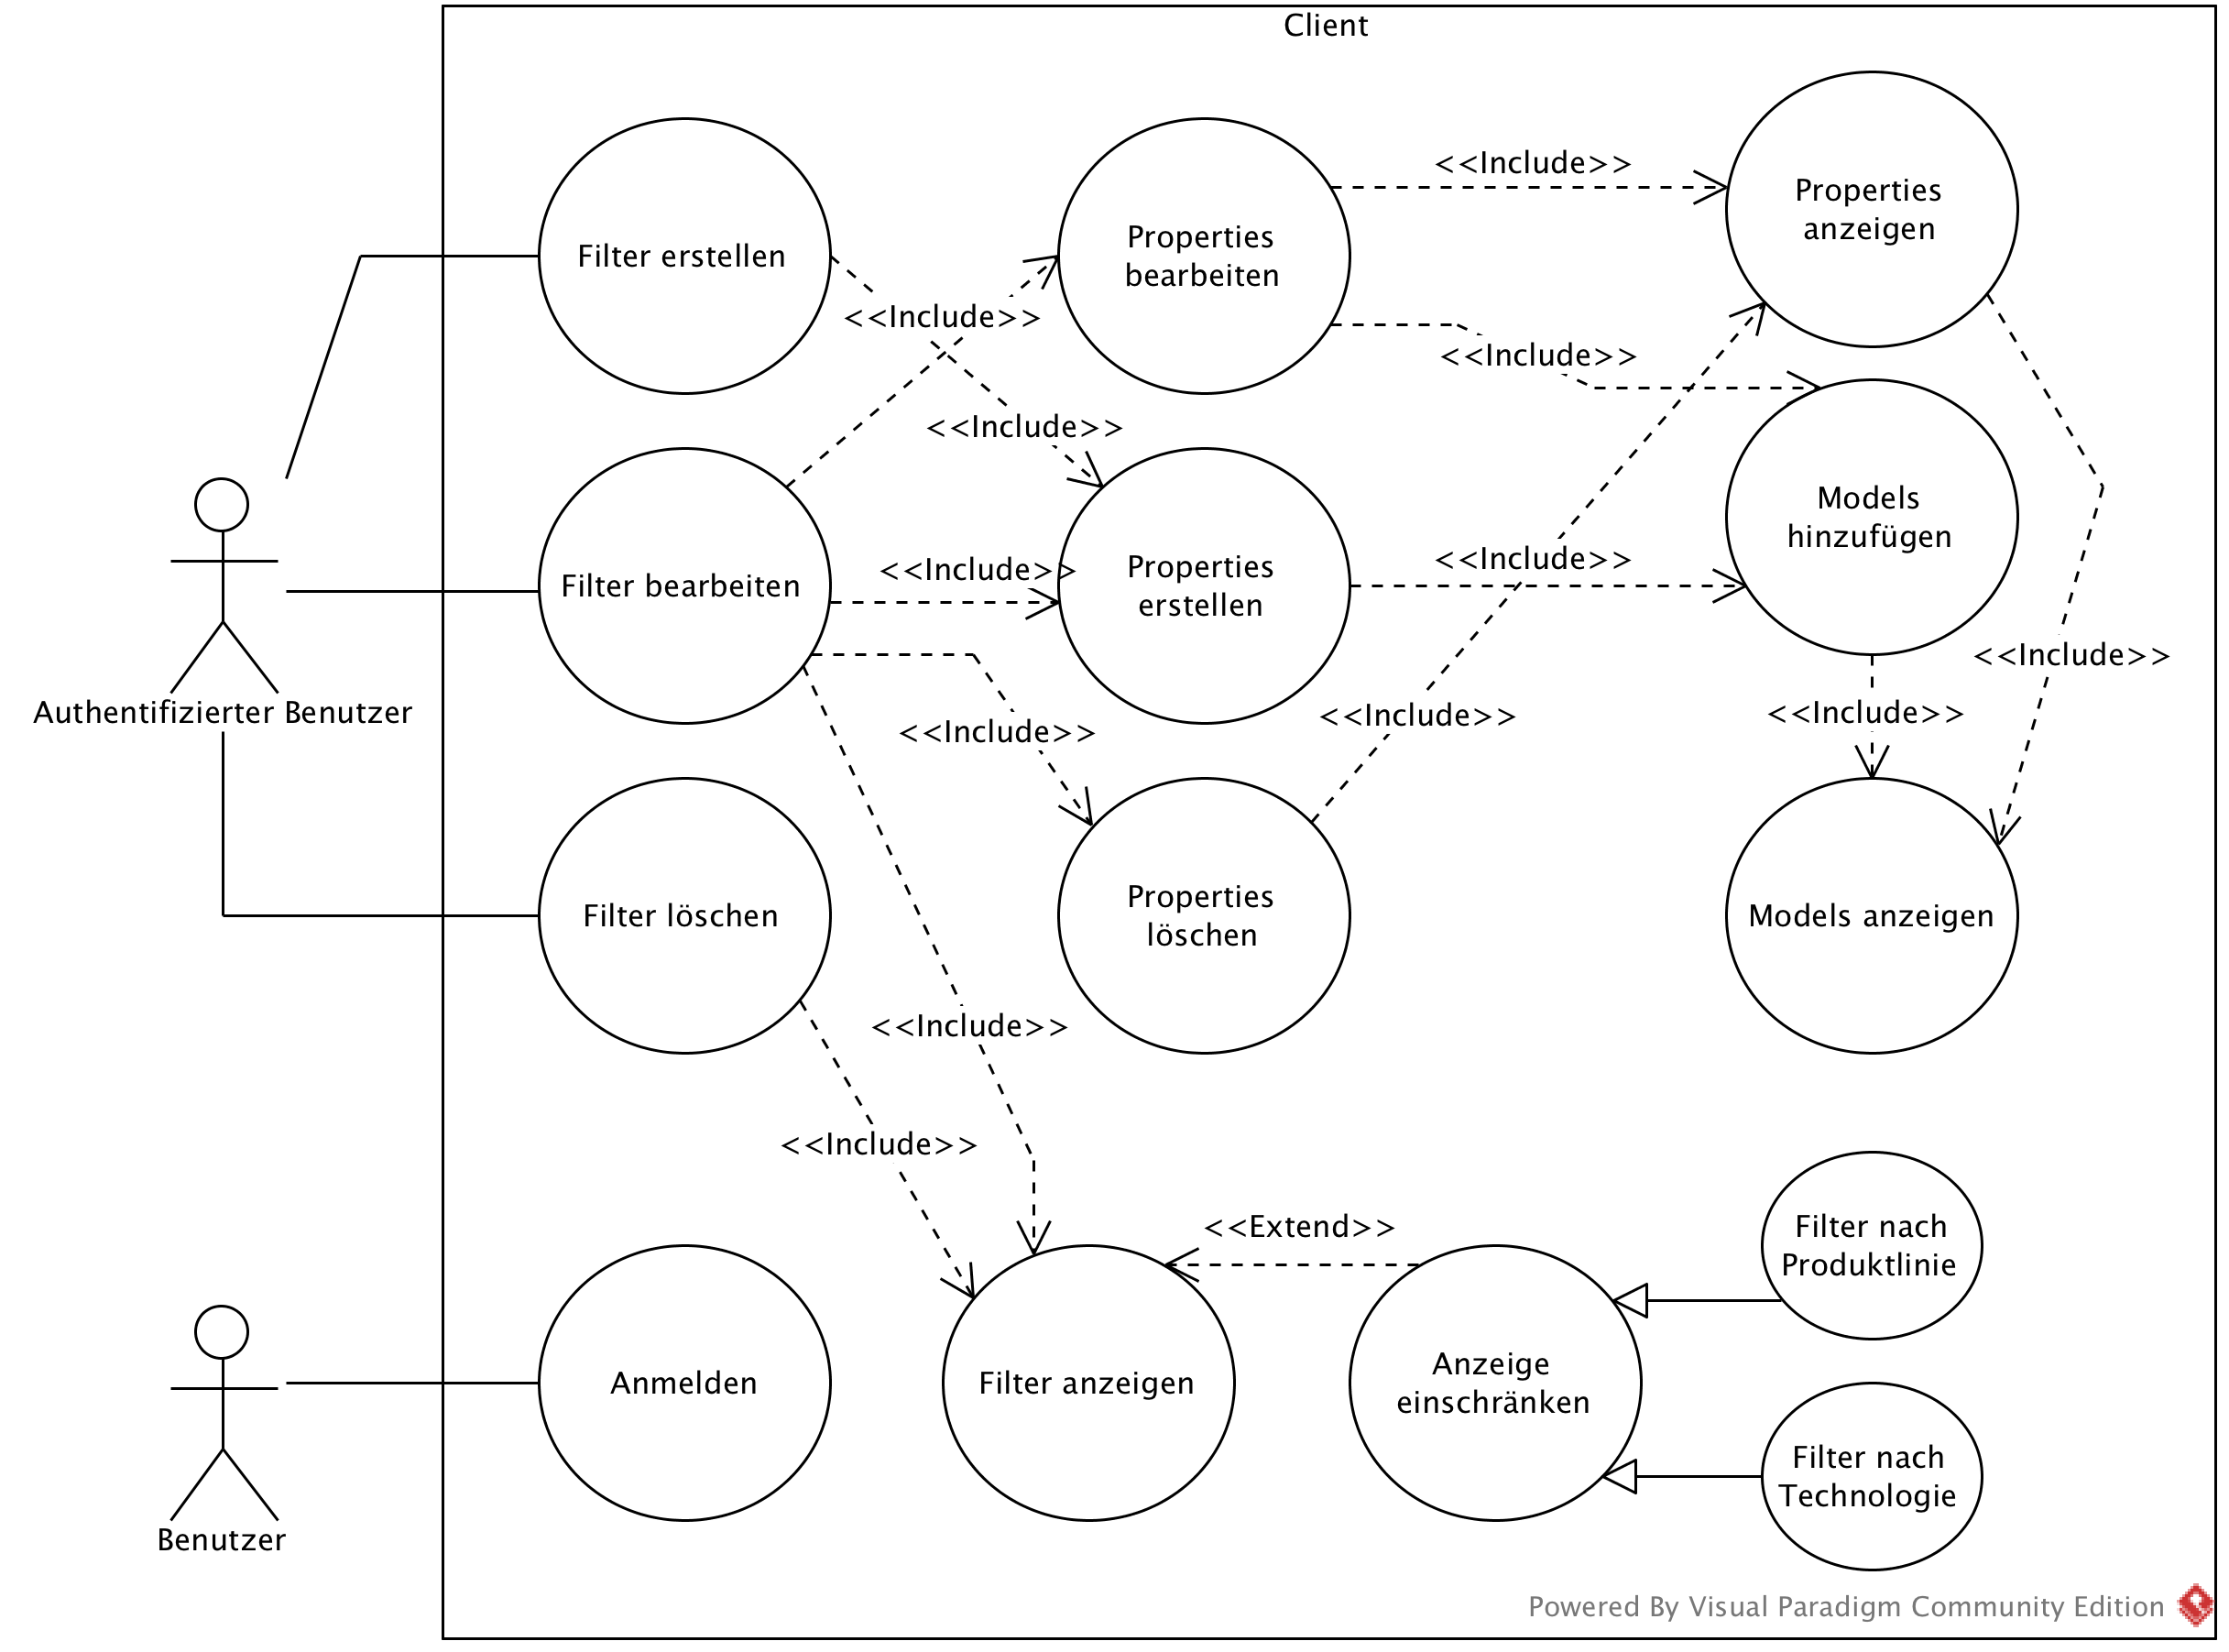
\includegraphics[width=.95\textwidth]{usecase} %{CS0031}
\caption{Anwendungsfalldiagramm}
\label{fig:usecase}
\end{figure}

Für das Verständnis der ermittelten Anwendungsfälle ist es notwendig, Filter als zentrale Objekte der Webanwendung zu verstehen. In Abschnitt \ref{sec:Zielsetzung} wurden Filter bereits als Elemente der Benutzeroberfläche eingeführt, denen eine komplexe Datenstruktur zugrunde liegt. Diese Datenstruktur beinhaltet sowohl Verknüpfungen zu Produkten und Produkteigenschaften, als auch layoutspezifische Daten, die das Erscheinungsbild in der Benutzeroberfläche bestimmen. Aufgrund dieser vielschichtigen Verknüpfungen können die Filter nur in Teilabschnitten bearbeitet werden. Dieser Sachverhalt wurde bei der Erarbeitung der Anwendungsfälle berücksichtigt und Abhängigkeiten modelliert.

\subsubsection{/F1.1/ Anmelden}

\begin{description}[leftmargin=8em,style=nextline]
\item[Akteure] Benutzer
\item[Includes] Keine
\item[Beschreibung]
Um die Anwendung zu nutzen, muss sich der Benutzer mit Benutzernamen und Passwort anmelden. Die Anmeldedaten müssen über eine Anmeldemaske eingegeben und anschließend verifiziert werden. Nach erfolgreicher Anmeldung muss der Benutzer in den geschützten Bereich der Webanwendung weitergeleitet werden.
\end{description}

\subsubsection{/F2.1/ Filter anzeigen}

\begin{description}[leftmargin=8em,style=nextline]
\item[Akteure] Authentifizierter Benutzer
\item[Includes] Keine
\item[Beschreibung]
Filtersteuerelemente müssen dem Benutzer angezeigt werden. Die Anwendung generiert die Filtersteuerelemente anhand der Filterdaten und orientiert sich dabei am Layout des FlowConfigurator. Die Anzeige muss zusätzlich Schaltflächen für die auf die Filter anwendbaren Operationen enthalten (Bearbeiten, Löschen, Erstellen).
\end{description}

\subsubsection{/F2.2/ Filteranzeige einschränken}

\begin{description}[leftmargin=8em,style=nextline]
\item[Akteure] Authentifizierter Benutzer
\item[Extends] F2.1 
\item[Beschreibung]
Der Benutzer muss die Möglichkeit haben, die angezeigten Filter einzuschränken. Die Filterung soll nach Technologie und Produktlinie möglich sein. Die Anwendung zeigt dazu entsprechende Steuerelemente an.
\end{description}

\subsubsection{/F2.3/ Filter erstellen}

\begin{description}[leftmargin=8em,style=nextline]
\item[Akteure] Authentifizierter Benutzer
\item[Includes] F3.3
\item[Beschreibung]
Der Benutzer kann neue Filter hinzufügen. Die Anwendung stellt dem Benutzer zu diesem Zweck Dateneingabemasken zur Verfügung. Das Hinzufügen der Filter erfolgt in Teilabschnitten, durch die der Benutzer geführt wird:

\begin{itemize}
\item Die Filtergruppe muss festgelegt werden (Basis- oder Spezialfilter)
\item Der Filtertyp muss bestimmt werden (Boolean oder Listenfilter) 
\item Geräteeigenschaften und Sensoren, nach denen gefiltert werden soll, müssen bestimmt bzw. verknüpft werden
\end{itemize}

\end{description}

\subsubsection{/F2.4/ Filter bearbeiten}

\begin{description}[leftmargin=8em,style=nextline]
\item[Akteure] Authentifizierter Benutzer
\item[Includes] F2.1, F3.2, F3.3, F3.4
\item[Beschreibung]
Der Benutzer muss existierende und neu angelegte Filter vollumfänglich bearbeiten können. Dazu werden von der Anwendung Dateneingabemasken angeboten. Zusätzlich soll auch die Anordnung der Filtersteuerelemente in der Benutzeroberfläche anpassbar sein. 
\end{description}

\subsubsection{/F2.5/ Filter löschen}

\begin{description}[leftmargin=8em,style=nextline]
\item[Akteure] Authentifizierter Benutzer
\item[Includes] F2.1
\item[Beschreibung]
Der Benutzer muss Filter über die Benutzeroberfläche löschen können. Dazu werden entsprechende Schaltflächen in der Filterübersicht angezeigt.
\end{description}

\subsubsection{/F3.1/ Properties anzeigen}

\begin{description}[leftmargin=8em,style=nextline]
\item[Akteure] Authentifizierter Benutzer
\item[Includes] F4.1
\item[Beschreibung]
Properties müssen in der Benutzeroberfläche angezeigt werden. Der Benutzer muss die Möglichkeit haben über Schaltflächen Aktionen auf den Properties auszuführen (Bearbeiten, Löschen, Erstellen).
\end{description}

\subsubsection{/F3.2/ Properties bearbeiten}

\begin{description}[leftmargin=8em,style=nextline]
\item[Akteure] Authentifizierter Benutzer
\item[Includes] F4.1, F4.2
\item[Beschreibung]
Properties beziehen sich auf Sensorspezifikationen, nach denen gefiltert werden soll. Der Benutzer muss vorhandene Properties eines Filters über eine Dateneingabemaske bearbeiten können.
\end{description}

\subsubsection{/F3.3/ Properties erstellen}

\begin{description}[leftmargin=8em,style=nextline]
\item[Akteure] Authentifizierter Benutzer
\item[Includes] F4.2
\item[Beschreibung]
Der Benutzer muss ebenso neue Properties zu einem Filter hinzufügen können. Die Anwendung stellt zu diesem Zweck eine Dateneingabemaske zur Verfügung.
\end{description}

\subsubsection{/F3.4/ Properties löschen}

\begin{description}[leftmargin=8em,style=nextline]
\item[Akteure] Authentifizierter Benutzer
\item[Includes] F3.1
\item[Beschreibung]
Der Benutzer muss Properties über die Benutzeroberfläche löschen können. Dazu werden entsprechende Schaltflächen in der Property-Übersicht angezeigt.
\end{description}

\subsubsection{/F4.1/ Models anzeigen}

\begin{description}[leftmargin=8em,style=nextline]
\item[Akteure] Authentifizierter Benutzer
\item[Includes] Keine
\item[Beschreibung]
Alle verfügbaren Models müssen aufgelistet werden. Aufgrund der Vielzahl der Models müssen diese für den Benutzer organisiert werden. Zu diesem Zweck stellt die Anwendung eine mehrseitige und sortierbare Tabelle bereit. 
\end{description}

\subsubsection{/F4.2/ Models hinzufügen}

\begin{description}[leftmargin=8em,style=nextline]
\item[Akteure] Authentifizierter Benutzer
\item[Includes] F4.1
\item[Beschreibung]
Models sind Sensoren, die mit einer Property verknüpft werden. Der Benutzer muss bestehende Models mit einer Property verknüpfen können. Die Anwendung stellt dafür eine Übersicht zur Verfügung, die es den Benutzer erlaubt über eine Checkbox Models an- und abzuwählen.
\end{description}

\section{Nichtfunktionale Anforderungen}
\label{sec:Analyse:Nichtfuntionale Anforderungen}

Neben der Umsetzung der funktionalen Anforderungen, sollen für die Umsetzung der zu entwickelnden Webanwendung folgende Qualitätsanforderungen beachtet werden:

\subsubsection{Performance}

Aufgrund des Umfangs der zu bearbeitenden Daten und die zu erwartenden Latenzen ist es notwendig, die Schnittstelle möglichst leichtgewichtig zu konzipieren. Weiterhin ist es notwendig, Geschäftsprozesse weitestgehend serverseitig zu realisieren. Serverseitige Ressourcen sollen bei Bedarf skaliert werden können, um die Performance zu verbessern.

\subsubsection{Benutzbarkeit und Layout}
\label{sec:Analyse:Benutzbarkeit und Layout}

Gemessen am Funktionsumfang sollte die zu entwickelnde Webanwendung ein möglichst simples, strukturiertes und bedienerfreundliches Layout besitzen. Das Layout soll sich dabei allgemein an dem der FlowConfigurator Software orientieren, um für den Benutzer ein gewohntes Umfeld zu schaffen. Eine Besonderheit ergibt sich durch das anzuwendende \ac{WYSIWYG}-Prinzip: Die Anzeige und Darstellung der Filtersteuerelemente in der Filterübersicht müssen hinsichtlich der Anordnung und Gruppierung möglichst exakt der Benutzeroberfläche des FlowConfigurator entsprechen. Nach dem Rückführen der Filterdaten in den FlowConfigurator müssen die Filtersteuerelemente dort genau so ausgeprägt und angeordnet sein, wie sie der Benutzer zuvor in der Webanwendung vorgefunden hat.

Die neu zu gestaltenden Dateneingabemasken sollen für die jeweiligen Anwendungsfälle (siehe Abschnitt \ref{sec:Funktionale Anforderungen}) auf eigenen Unterseiten bereitgestellt werden, die über eine Navigation miteinander verknüpft sind. Dabei gilt es eine gewisse Konsistenz hinsichtlich des Aussehens und der Bedienung zu gewährleisten. 

\subsubsection{Sicherheit}

Da es sich bei den zu verarbeitenden Daten um nicht öffentliche Geschäftsdaten handelt, muss die Webanwendung Mechanismen zur Absicherung implementieren. Der Benutzer muss sich mit Benutzernamen und Passwort an der Webanwendung anmelden, um diese zu nutzen. Zusätzlich muss der Zugriff auf die Schnittstelle, welche die Daten zur Verfügung stellt, serverseitig abgesichert werden um Missbrauch vorzubeugen.

\subsubsection{Portabilität}

Die Webanwendung soll so konzipiert werden, dass die einzelnen Komponenten austauschbar sind. Das bedeutet, dass in jedem Fall eine lose Kopplung zwischen Komponenten gegeben sein soll. Die Schnittstellenspezifikation sollte aus diesem Grund allgemein gehalten werden, um eine Wiederverwendbarkeit in möglichen Folgeprojekten zu gewährleisten.

Zusätzlich soll die Benutzeroberfläche auf verschiedenen Bildschirmgrößen korrekt dargestellt werden. Der Schwerpunkt liegt aber in der Unterstützung gebräuchlicher Desktop-Bildschirmgrößen.

\section{Technologiebewertung und -entscheidung}
\label{sec:Analyse:Technologiebewertung und -entscheidung}

\subsection{Server}
\label{sec:Analyse:Server}

Für die Realisierung der Anwendung müssen einige technologische Grundvoraussetzungen erfüllt werden. Die ermittelten Kriterien werden in Tabelle \ref{tab:Technologiebewertung} mit den ausgewählten Plattformen NodeJS, PHP und C\# (CSharp) abgeglichen. Die Auswahl der Plattformen, die zum Vergleich herangezogen werden, erfolgt anhand von Kenntnissen und Erfahrungen, die der Autor dieser Arbeit bereits mit den Plattformen gemacht hat. Objektiv betrachtet gibt es natürlich auch noch weitere infrage kommende Plattformen, wie zum Beispiel Java oder Ruby on Rails. Aufgrund des begrenzten Zeitrahmens dieser Arbeit ist es aber notwendig, Vorkenntnisse des Autors zu berücksichtigen, um eine möglichst zeiteffiziente Entwicklung zu gewährleisten. Der Vergleich konkreter Frameworks entfällt, da es ausschließlich um die Bewertung technischer Grundvoraussetzungen geht.

\begin{table}[H]
\centering
\def\rr{\rightskip=0pt plus1em \spaceskip=.3333em \xspaceskip=.5em\relax}
\setlength{\tabcolsep}{1ex}
\def\arraystretch{1.20}
\setlength{\tabcolsep}{1ex}
\small
\begin{tabular}{|r||c|c|c|} \hline
& \emph{NodeJS} & \emph{PHP} & \emph{C\#} \\
\hline\hline
MSSQL-Unterstützung & \checkmark & \checkmark & \checkmark \\
\hline
Plattformunabhängigkeit & \checkmark & \checkmark & $\times$ \\
\hline
Database First & \checkmark & \checkmark & \checkmark \\
\hline
\end{tabular}
\caption{Technologiebewertung auf Grundlage technischer Grundanforderungen}
\label{tab:Technologiebewertung}
\end{table}

\subsubsection{MSSQL-Unterstützung}

Die bereitgestellte Datenbank basiert auf \acf{MSSQL}. Deshalb ist es notwendig, dass die ausgewählte Technologie, Treiber zum Ansprechen dieser Datenbank bereitstellt. Diese Anforderung wird Unteranderem auch gestellt, weil eine MSSQL-Datenbank im Umfeld einer Webanwendung einen geringeren Verbreitungsgrad hat und eine Treiber-Unterstützung daher nicht selbstverständlich ist. Alle zum Vergleich stehenden Technologien erfüllen formal diese Anforderung. Die Treiberunterstützung unter C\# ist dabei aufgrund der Nähe zum Microsoft-Ökosystem sehr robust und unterstützt auch die aktuellsten SQL-Server Versionen. Der MSSQL-Treiber für NodeJS und PHP bauen beide auf dem \ac{TDS} Protokoll auf, das ursprünglich von Sybase entwickelt und später von Microsoft übernommen wurde. Es gibt verschiedene Ausbaustufen des Protokolls und auch Open-Source Ableger, wie zum Beispiel FreeTDS. Die \ac{MSSQL}-Treiber für PHP und NodeJS werden aber direkt von Microsoft bereitgestellt.

\subsubsection{Plattformunabhängigkeit}

Die Entwicklung unter C\# impliziert die Bindung an das Microsoft-Ökosystem. Entwicklungsumgebung, Technologiestack und Serverbetriebssystem werden dabei vorgegeben. Daraus ergeben sich die Nachteile, dass die Entwicklung der Anwendung nur unter dem Windows Betriebssystem stattfinden kann und eine Windows-Serverumgebung für die Bereitstellung der Anwendung benötigt wird. Auf NodeJS und PHP basierende Plattformen können unter allen gängigen Betriebssystemen entwickelt werden. Die Bereitstellung kann dabei auf vergleichsweise günstigen Linux-Servern erfolgen.

\subsubsection{Database First}

\ac{ORM} ist eine Technik der Softwareentwicklung, mit der eine, in einer objektorientierten Programmiersprache programmierte, Anwendung, Objekte in einer relationalen Datenbank ablegen kann. Die Anwendung sieht die Datenbank dann als objektorientierte Datenbank, was die Programmierung erleichtert. \parencite[vgl.][511]{Vogel2011} Die Implementierung eines \ac{ORM}-Frameworks ist generell für alle Anwendungen mit objektorientiertem Hintergrund empfehlenswert. Im Kontext dieser Arbeit ergibt sich aber eine Besonderheit. Es existiert bereits eine umfangreiche Datenbasis, aus denen ORM-Modelklassen abgeleitet werden müssen. Aufgrund des vergleichsweise großen Umfangs ist es aufwendig, diese Klassen händisch anzulegen. Eine Modelklasse modelliert neben Attributen, Relationsschemata und Relationsnamen auch die Beziehungen zu anderen Tabellen, die je nach Datenbasis sehr komplex ausfallen können. Diese Beziehungen aus einer bestehenden Datenbasis händisch in die entsprechenden Modelklassen zu übertragen würde viel Zeit in Anspruch nehmen und aufgrund der Komplexität zu Fehlern führen. Deshalb ist es notwendig, die Modelklassen aus der Datenbank vollautomatisch zu generieren. Dieses Prinzip wird auch als Database First bezeichnet und von den meisten ORM-Frameworks bereits nativ unterstützt. In Fällen, wo keine native Unterstützung vorgesehen ist, gibt es zahlreiche Erweiterungen für bekannte ORM-Frameworks, die sich dieser Problematik widmen.

NodeJS bietet mit der Bibliothek sequelize-Auto eine Erweiterung für das ORM-Framework sequelize an. Das umfangreiche Entity-Framework auf Basis von C\# bietet von Haus aus eine Funktion zur Generierung von Models aus einer Datenbank. Das in der PHP-Welt weitverbreitete Doctrine ORM-Framework bietet ebenfalls native Unterstützung zur Generierung der Modelklassen an. Weiterhin gibt es auch Erweiterungen für das PHP-basierte Eloquent ORM-Framework.

\subsection{Client}
\label{sec:Analyse:Client}

Der Webclient wird ausschließlich über eine einheitliche Schnittstelle mit dem Server kommunizieren. Daher haben die Technologieanforderungen, die für die Serverkomponenten ermittelt wurden, keine Auswirkung auf die Technologieentscheidung des Webclients. Als Kommunikationsprotokoll kommt für Webanwendungen standardmäßig \ac{HTTP} zum Einsatz. Die Benutzeroberfläche wird mittels HTML, CSS und Javascript realisiert. Damit ergeben sich keine besonderen Anforderungen bezüglich des eingesetzten Frameworks. Populäre Javascript Frameworks wie zum Beispiel AngularJS, Ember oder Backbone eignen sich alle gleichermaßen gut, um sowohl die Schnittstelle anzusprechen, als auch die ermittelten funktionalen und nichtfunktionalen Anforderungen umzusetzen. Javascript wird heutzutage aber nicht mehr nur eingesetzt um Benutzerinteraktionen auszuwerten, Inhalte zu verändern, nachzuladen oder zu generieren und so die Möglichkeiten von HTML und CSS zu erweitern, sondern findet auch außerhalb von Browsern als Servertechnologie Anwendung. Daraus ergeben sich Synergien mit der in Abschnitt \ref{sec:Analyse:Server} betrachteten serverseitigen NodeJS Plattform, die ebenfalls auf Javascript basiert. Der Einsatz ein und derselben Sprache für die Entwicklung von Client und Server kann die Realisierung aufgrund des geteilten Technologie-Stacks\footnote{Ein Technologie-Stack bezeichnet alle in einem Projekt benutzten Technologien} beschleunigen, da die Komplexität verringert und Abhängigkeiten reduziert werden.

\subsection{Machbarkeitsstudie}

Die in Abschnitt \ref{sec:Analyse:Server} gewonnenen Erkenntnisse aus dem Vergleich von ausgewählten Serverplattformen basieren lediglich auf Recherchen und sind damit nicht verifiziert. Vor allem wenn für die Sicherstellung technischer Grundvoraussetzungen im Rahmen der Projektanforderungen Open-Source Bibliotheken eingesetzt werde müssen, kann auf die versprochenen Funktionalitäten nicht uneingeschränkt vertraut werden. Das kann sowohl an unvollständigen Dokumentationen liegen, die keine gesicherten Rückschlüsse auf die benötigte Funktionalität zulassen, als auch an Unzuverlässigkeiten und Fehlern in den Implementierungen.

Um die Erkenntnisse aus der Technologierecherche zu verifizieren ist es notwendig die getätigten Annahmen anhand von prototypischen Implementierungen zu überprüfen. Als Schwerpunkt wird dabei die MSSQL Treiberunterstützung und die Generierung der ORM-Modelklassen nach dem Database First Prinzip getestet. Dabei gibt es keinen speziellen Projektrahmen; es werden stets nur die nötigsten Voraussetzungen geschaffen um eine gesicherte Annahme über die Funktionsfähigkeit der zu testenden Implementierungen tätigen zu können. Dabei kommen sogenannte \emph{Seeds} zum Einsatz. Als Seeds im Kontext der Software-Entwicklung werden vorkonfigurierte Projekte bezeichnet, die für nahezu alle populären Plattformen und Frameworks zur Verfügung stehen. Diese Projekte implementieren bereits benötigte Abhängigkeiten, die für die Realisierung vieler Projekte ohnehin gebraucht werden. Meist sind das Implementierungen für den Zugriff auf Datenbanken, darauf aufbauende rudimentäre Benutzerauthentifizierung, sowie einfache HTML-Templates. Dieses Vorgehen beschleunigt die Machbarkeitsstudie, da keine komplizierten Projektkonfigurationen vorgenommen werden müssen.

\subsubsection{NodeJS}

Für den Test der MSSQL-Anbindung wurde das Beispielprojekt \emph{express-example}\footnote{Siehe \hyperlink{https://github.com/sequelize/express-example}{https://github.com/sequelize/express-example}} verwendet. Express, ist der dabei der Name eines serverseitigem Frameworks auf Basis von NodeJS. Dieses Projekt beinhaltet das ebenfalls auf NodeJS basierende ORM-Framework \emph{sequelize}. Das Projekt ist für die Benutzung einer MySQL-Datenbank vorkonfiguriert. Die benötigten Treiber für die MSSQL-Unterstützung müssen nachinstalliert werden. Es wird dabei der offiziell von Microsoft bereitgestellten Treiber für NodeJS verwendet.

Nach der erfolgreichen Installation muss die im Projekt enthaltende Konfigurationsdatei mit den Verbindungsdaten der bereitgestellten Testdatenbank erweitert werden. Der Datenbankdialekt wird außerdem von MySQL auf MSSQL geändert. Die Testdatenbank ist eine Spiegelung der von der netbase Gmbh zur Verfügung gestellten Datenbank. Für den Test der Datenbankanbindungen werden jeweils nur sehr einfache Abfragen zum Lesen, Schreiben und Löschen von Datensätzen implementiert. Die Tests ergeben eine fehlerfreie Funktion der verwendeten MSSQL-Treiber.

Als nächstes wird zum Test des Database First Prinzips das Projekt um das Paket \emph{sequelize-auto} erweitert. Laut Dokumentation soll es damit möglich sein, ORM-Modelklassen auf Grundlage der Testdatenbank zu generieren. Angesteuert wird die Bibliothek innerhalb der Projektumgebung über die Kommandozeile, indem die korrekten Verbindungsdaten übergeben werden. Als Ergebnis des Tests werden zwar alle ORM-Modelklassen mit den korrekten Schemata generiert, aber es fehlt die Modellierung der Beziehung der Tabellen. Dieser Sachverhalt ist aus der Dokumentation nicht ersichtlich und konnte anhand weiterer Recherchen als fehlendes Feature identifiziert werden. Es können außerdem keine alternativen Bibliotheken zur Bereitstellung der benötigten Funktionalität gefunden werden.

\subsubsection{PHP}

Als Ausgangsbasis für die PHP-Tests dient das Framework Laravel. Die MSSQL-Treiberunterstützung wird auf Basis des im Laravel Framework enthaltenen ORM-Frameworks \emph{Eloquent} getestet. Verwendet wird der offizielle von Microsoft bereitgestellte MSSQL-Treiber. Die Basis der Testumgebung bildet PHP in der Version 5.6.24. Es werden ebenfalls einfache Abfragen zum Lesen, Schreiben und Löschen von Datensätzen implementiert. Dabei kann eine einwandfreie Treiberunterstützung verifiziert werden.

Für die Generierung der Modelklassen wird das Projekt um die Bibliothek \emph{laravel-model-generator} erweitert. Diese Bibliothek wird ebenfalls über die Kommandozeile angesprochen und bietet umfangreiche Einstellungsmöglichkeiten, die eine feingranulare Konfiguration der zu generierenden ORM-Modelklassen zulässt. Die Modelklassen können generiert werden und modellieren nach einer stichprobenartigen Kontrolle die korrekten Schemata und Beziehungen der Testdatenbank. Ein Problem konnte bei der Modellierung von zusammengesetzten Primärschlüsseln identifiziert werden. Diese fehlen bei der Generierung und müssen händisch nachgetragen werden.

\subsection{Ergebnis}

Anhand der in Abschnitt \ref{sec:Analyse:Technologiebewertung und -entscheidung} getätigten theoretischen Bewertungen technologischer Grundvoraussetzungen und der im Anschluss durchgeführten Machbarkeitsstudie konnte eine Entscheidung hinsichtlich der einzusetzenden Technologie getroffen werden. Die Entwicklung des Prototyps mit C\# kann aufgrund der vom Autor aufgestellten Anforderung der Plattformunabhängigkeit nicht erfolgen. Die Plattform NodeJS bietet interessante Synergien zwischen einem auf Javascript basierenden Client-Frontend und einer ebenfalls auf Javascript basierenden Serverplattform. Die getätigte Annahme über die Unterstützung des Database First Prinzips konnte allerdings mittels der durchgeführten Machbarkeitsstudie widerlegt werden. Die für die Serverplattform PHP getätigten Annahmen und die erfolgreich verlaufende Machbarkeitsstudie führt zu der Entscheidung PHP als Serverplattform einzusetzen. Aufgrund der Erfahrungen des Autors und der vielversprechend verlaufenden Machbarkeitsstudie wird das PHP Framework Laravel die Basis der Serverkomponente bilden.

Für die Realisierung des Frontend kommt AngularJS als Javascript-Framework zum Einsatz. Die Entscheidung beruht auf den bereits gemachten positiven Erfahrungen des Autors mit AngularJS und den unkritischen technologischen Anforderungen. Es ist anzumerken, dass auf Grundlage der gestellten Anforderungen, auch die in Abschnitt \ref{sec:Analyse:Client} genannten Alternativen hätten eingesetzt werden können.
\chapter{Entwurf}
\label{cha:Entwurf}

In diesem Kapitel wird auf Grundlage der in Kapitel \ref{cha:Anforderungsanalyse} vorgenommenen Anforderungsanalysen ein Systementwurf der zu realisierenden Webanwendung entworfen. Zu diesem Zweck wird die geplante Systemarchitektur anhand eines Komponentendiagramms erläutert, sowie das zugrunde liegende Datenmodell beschrieben. Außerdem werden die Überlegungen zur Gestaltung der Benutzeroberfläche diskutiert und dabei Bezug auf das Prinzip WYSIWYG genommen.

\section{System-Architektur}

Die zu entwickelnde Webanwendung realisiert eine typische Client-Server-Architektur auf Basis eines RESTful Webservice. Konkret kann die Architektur deshalb auch als \acf{ROA} typisiert werden (siehe Abschnitt \ref{sec:ROA}). Das in Abbildung \ref{fig:architecture} dargestellte Komponentendiagramm beinhaltet die wesentlichen Komponenten, Schnittstellen und deren Beziehungen zueinander, die für die Realisierung der Anwendung benötigt werden. Nachfolgend wird mit Bezug auf die Abbildung \ref{fig:architecture} die entworfene Architektur getrennt nach Server und Client erläutert. Dabei werden nur grundlegende Gedanken zum Entwurf diskutiert, da eine detaillierte Betrachtung der einzelnen Bestandteile im Kapitel \ref{cha:Implementierung} stattfindet.

\begin{figure}[H]
\centering
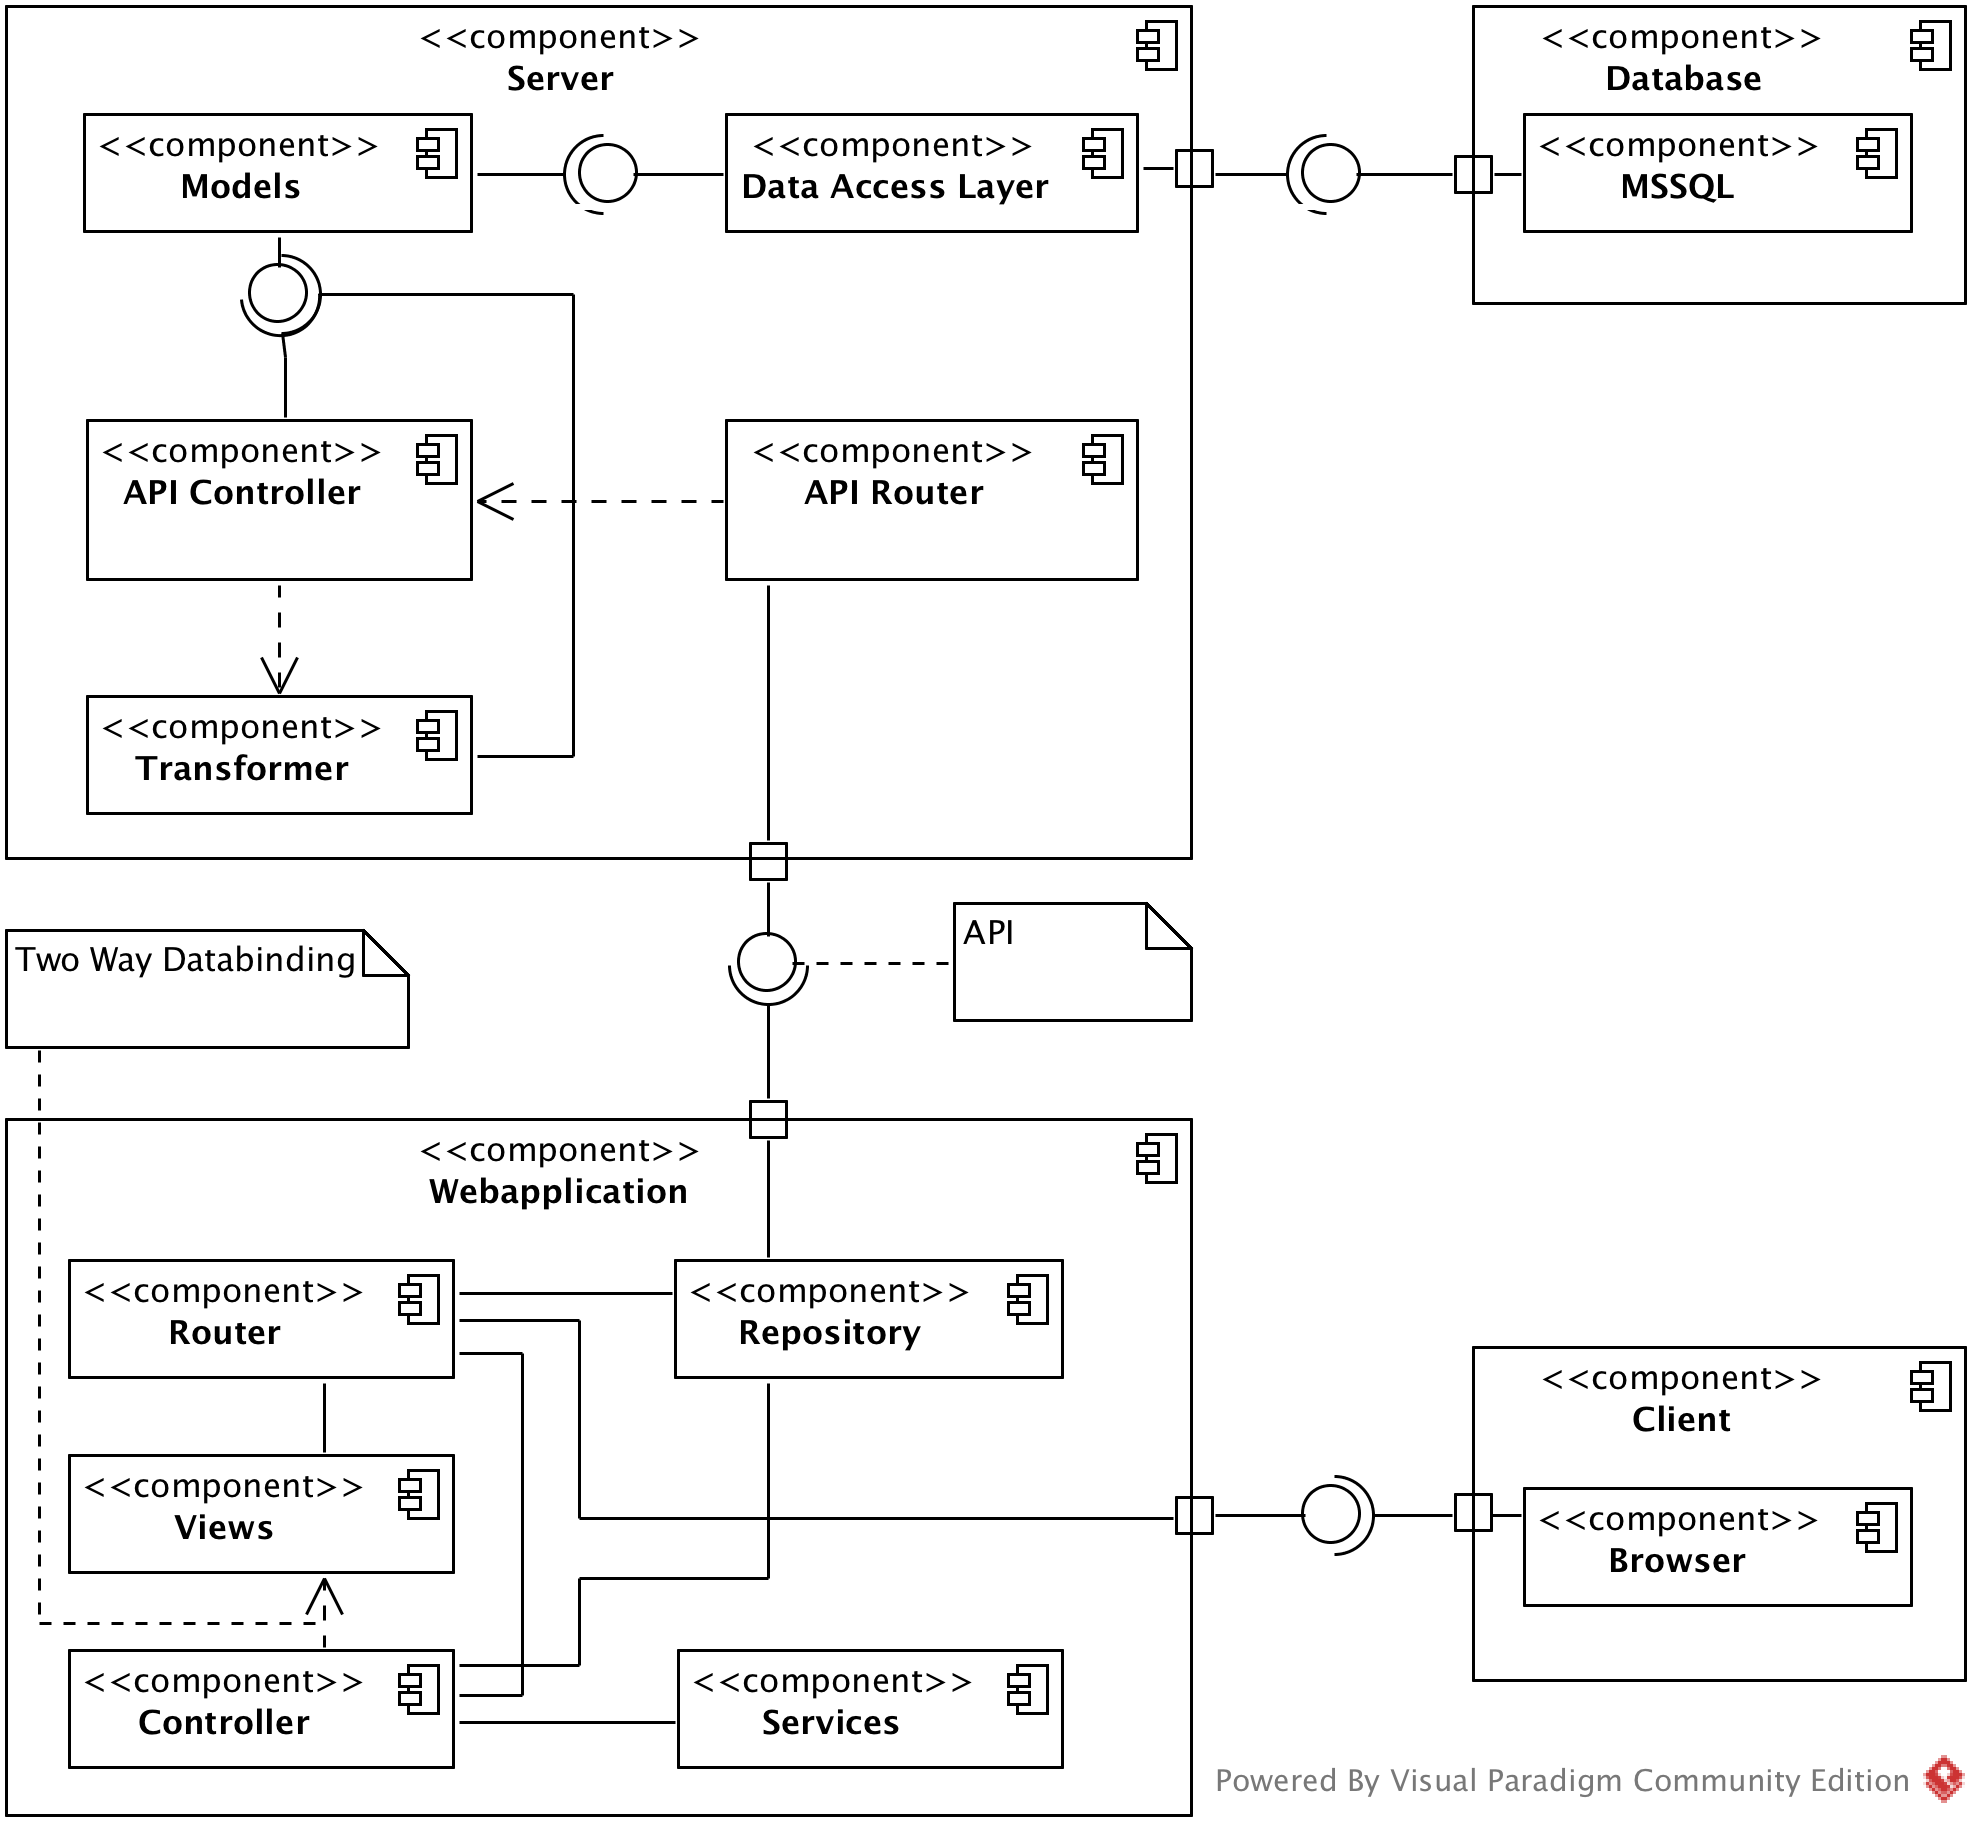
\includegraphics[width=1.0\textwidth]{architecture} %{CS0031}
\caption{Komponentendiagramm der Webanwendung}
\label{fig:architecture}
\end{figure}

\subsection{Server}
\label{sec:Entwurf:Server}

Hauptaufgabe des Server ist die Bereitstellung einer REST konformen Schnittstelle und die Realisierung einer Datenbankverbindung. Die Schnittstelle wird durch einen \emph{Router} implementiert, der alle aufrufbaren Endpunkte\footnote{Ein \acf{URI}, der einen eindeutigen Zugriff auf eine Ressource zulässt, wird auch als Endpunkt bezeichnet.} kapselt. Wird ein solcher Endpunkt aufgerufen, leitet der Router die Anfrage an einen zuständigen Controller weiter. Ein Controller implementiert Methoden, die die in Abschnitt \ref{sec:ROA:Einheitliche Schnittstelle} dargestellten HTTP-Methoden in ihrer Funktionsweise im Kontext einer REST konformen Schnittstelle widerspiegeln. Das bedeutet, dass die Controller im Wesentlichen für die Realisierung typischer Funktionen (Lesen, Schreiben, Löschen, Aktualisieren), die auf einer Ressource ausgeführt werden können, zuständig sind. Die dabei benötigte Kommunikation mit der zur Verfügung gestellten Datenbank erfolgt über eine \emph{Datenzugriffsschicht}, die mittels eines ORM-Frameworks realisiert wird. Das ORM-Framework erlaubt es \emph{Models} zu definieren, die jeweils eine Datenbanktabelle als Objekt beschreiben. Modelklassen beinhalten neben dem Schema der Tabelle auch Beziehungen, die über vom ORM-Framework bereitgestellte Methoden modelliert werden. Die Controller implementieren diese Modelklassen, mit Hilfe derer ein Zugriff auf die Datenbank erfolgen kann. Bevor die abgefragten Daten aber als Antwort über die Schnittstelle zurückgeschickt werden, findet eine Standardisierung und Homogenisierung statt. Dieser Vorgang ist notwendig, weil ansonsten ungefilterte Daten aus der Datenbank übertragen werden würden, die vom aufrufenden Client für die Realisierung seiner Aufgaben unter Umständen nicht alle benötigt werden oder im falschen Format vorliegen. Aus diesem Grund implementieren die Controller zusätzlich noch so genannte \emph{Transformer}. Diese werden mit dem Ergebnis aus dem Aufruf der Modelklassen, also mit Rohdaten aus der Datenbank, aufgerufen. Die Transformer definieren, welche Daten in welcher Form im Bezug auf die Rohdaten über die Schnittstelle übertragen werden sollen. Bei diesem Prozess wird unter anderem auch das Datenformat der Übertragung festgelegt. Zusätzlich verfügen die Transformer auch noch über die Möglichkeit, aus denen in den Modelklassen definierten Beziehungen, Daten aus verknüpften Tabellen in die Antwort einzubetten. Ist dieser Prozess abgeschlossen, werden die Daten als Antwort über den Router zurück an den Client geschickt.

\subsection{Client}
\label{sec:Entwurf:Client}

Der Client wird als \ac{SPA} auf Basis des AngularJS Frameworks realisiert. Eine \ac{SPA} zeichnet sich durch ein einziges HTML-Dokument aus, in dem Inhalte dynamisch nachgeladen werden können. Diese Art der Webarchitektur steht im Gegensatz zu klassischen Webanwendungen, welche aus mehreren, untereinander verlinkten HTML-Dokumenten bestehen, die meist vom Server bereitgestellt werden. Als zentrale Komponente dient der Webanwendung, wie auch schon dem Server, ein \emph{Router}. Dieser Router kapselt alle aufrufbaren Routen der Webanwendung und wird durch den Aufruf einer \ac{URL} aus einem Browser heraus angesteuert. Der Router setzt sich aus sogenannten \emph{States} zusammen. Ein State definiert neben der \ac{URL} einen zugehörigen \emph{Controller} und \emph{View}. Nach dem Aufruf eines States wird der angegebene Controller aufgerufen und der zugehörigen View in Form eines HTML-Dokuments in das \ac{DOM} geladen. Die States haben außerdem die Möglichkeit, sogenannte \emph{Resolves} zu implementieren. Das sind Abhängigkeiten, die vor dem Aufruf des Controllers und der Anzeige der View aufgelöst werden. Resolves können zum Beispiel Schnittstellenaufrufe zum Laden benötigter Daten implementieren. Der Vorteil liegt dabei darin begründet, dass der View tatsächlich erst angezeigt wird, wenn alle benötigten Daten geladen wurden und damit keine unvollständigen Seiten angezeigt werden. Der Aufruf der Schnittstelle wird durch ein \emph{Repository} gekapselt, in dem alle verfügbaren Endpunkte definiert sind. Das Repository ist faktisch das Gegenstück des API-Routers auf der Serverseite. Der Aufruf der Schnittstelle erfolgt mittels \ac{AJAX}. Das asynchrone Laden der Daten, hat den wesentlichen Vorteil, dass die Webanwendung während des Ladevorgangs benutzbar bleibt. Daten die als Resolve bereitgestellt werden, werden vom Router automatisch in den entsprechenden Controller injiziert. Ein Controller im Kontext von AngularJS ist nichts weiter als eine normale Javascript-Funktion. Eine Besonderheit ist nur die übergebene Variable \$scope. Mit dieser Variable können Daten mit dem View über eine bidirektionale Datenbindung ausgetauscht werden. Eine wesentliche Aufgabe von Controllern ist demnach die Bindung von Daten (die zum Beispiel über die Schnittstelle kommen können) an die \$scope Variable, um sie im View nutzbar zu machen. Daten, die an den Scope gebunden werden, bezeichnet man auch als \emph{Models}. Damit realisiert die Webanwendung ein klassische \ac{MVC} Architektur als Teil einer \acf{ROA} - wenn man das große ganze betrachtet. Eine weitere Komponente der Webanwendung bilden \emph{Services}. Services sind Klassen oder Funktionen die Business-Logik auf der Clientseite implementieren. Services können generell von allen Komponenten der Webanwendung genutzt werden.

\section{Datenbankmodell}
\label{sec:Entwurf:Datenbankmodell}

Die zur Verfügung gestellt Datenbank umfasst die vollständige Datenbasis der FlowConfigurator Software. Für die Realisierung der Webanwendung werden aber nicht alle Datenbanktabellen benötigt. Das in Abbildung \ref{fig:erdiagram} erarbeitete Datenbankschema beinhaltet die für die Realisierung der Webanwendung benötigten Tabellen.

\begin{figure}[H]
\centering

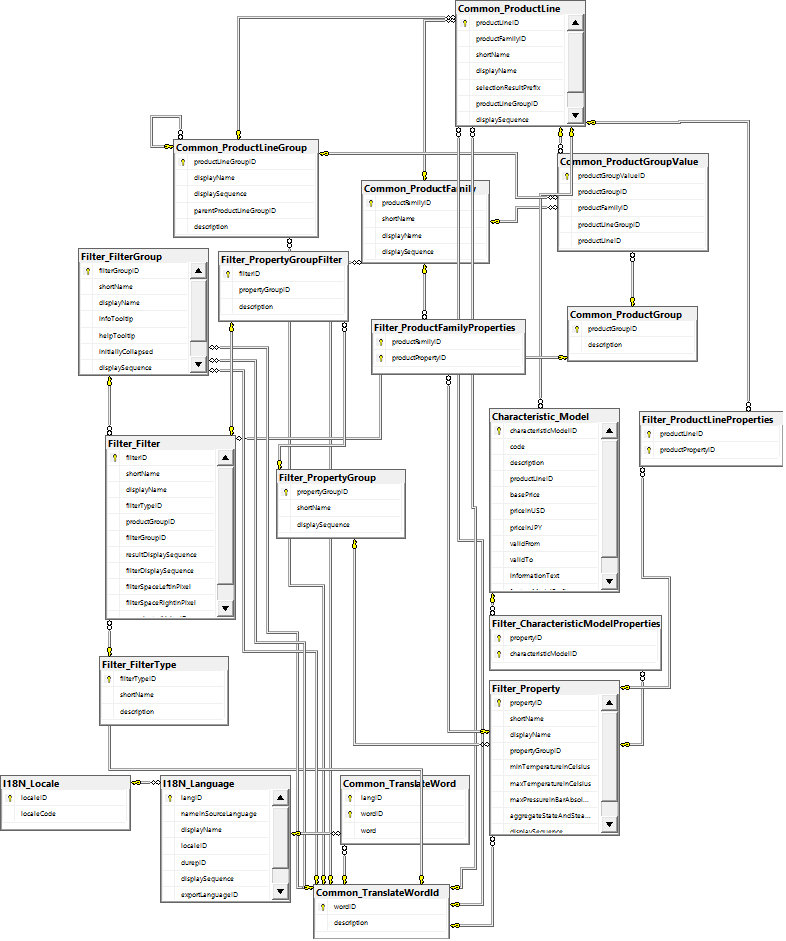
\includegraphics[width=1.0\textwidth]{er-diagram} %{CS0031}
\caption{Datenbankschema der Webanwendung}
\label{fig:erdiagram}
\end{figure}

Für das weitere Verständnis der Arbeit werden die ermittelten Tabellen nachfolgend aufgelistet und deren Inhalt und Beziehung beschrieben. Aufgrund der Komplexität der vorliegenden Datenstruktur kann dies nicht vollumfänglich und im Detail geschehen, sodass zusätzlich detailliertere Beschreibungen wichtiger Tabellen auch in aufbauenden Kapiteln erfolgen.

\subsubsection{Filter}

Die Filtertabelle ist die Ausgangstabelle der Filterabstraktion und beinhaltet layoutspezifische Daten zur Darstellung und Anordnung der Filtersteuerelemente. Ebenso werden Beziehungen zu FilterGroups, FilterTyps und PropertyGroupFilter hergestellt.

\subsubsection{FilterGroup}

Filtergruppen sind Bestandteil der layoutspezfischen Merkmale eines Filtersteuerelements. Es wird zwischen Basis- und erweiterten Filtern unterschieden. Diese Unterscheidung kommt bei der Anordnung der Filtersteuerelemente zum tragen.

\subsubsection{FilterTyp}

Ein Filtertyp bezeichnet die Ausprägung des Filtersteuerelements. Es wird zwischen Schaltern (Checkboxen) und Dropdown-Listen unterschieden.

\subsubsection{PropertyGroupFilter}

Die PropertyGroupFilter-Tabelle beschreibt eine Art der Filterung nach Properties. Sie ist eine Verknüpfungstabelle und stellt die Beziehung zur Filter-Tabelle und PropertyGroup-Tabelle her.

\subsubsection{PropertyGroup}

Die PropertyGroup-Tabelle beinhaltet übergreifende Sensormerkmale, nach denen gefiltert werden soll. Sie realisiert außerdem die Beziehung zur Property-Tabelle.

\subsubsection{Property}

Die Property-Tabelle beinhaltet konkrete Gerätevorgaben, d.h. Geräteeigenschaften, nach denen bei der Anwendung eines Filters entsprechend der Vorgabe passende Sensoren ermittelt werden.

\subsubsection{ProductLineProperty}

Bestimmte Geräteeigenschaften sind auf eine gesamte Produktlinie anwendbar. Die ProductLineProperty-Tabelle ist eine Verknüpfungstabelle und stellt die Beziehung zwischen einer Property und einer Produktlinie her.

\subsubsection{ProductFamilyProperty}

Wenige zu filternde Geräteeigenschaften treffen sogar auf alle Produkte innerhalb einer Produktfamilie zu. Die ProductFamilyProperty-Tabelle ist ebenfalls eine Verknüpfungstabelle, die die Beziehung zwischen einer Property und einer Produktfamilie realisiert.

\subsubsection{CharacteristicModel}

Die CharacteristicModel-Tabelle enthält die zu bestimmenden Models. Models beschreiben dabei Sensoren, die einer Produktlinie zugeordnet werden können. Als Besonderheit referenziert die CharacteristicModel-Tabelle auf sich selbst, so das Verschachtelungen der Models möglich sind.

\subsubsection{CharacteristicModelProperties}

Die CharacteristicModelProperties-Tabelle ist eine Verknüpfungstabelle, welche die Beziehung zwischen einer Property und einem CharacteristicModel realisiert. Sie beinhaltet also die Information, welche spezifizierten Geräteeigenschaften tatsächlich auf ein oder mehrere CharacteristicModels anwendbar sind.

\subsubsection{ProductFamily}

Produkte werden kategorisiert und gehören unter anderem einer Produktfamilie an. Die ProductFamily-Tabelle realisiert die Beziehung zu Produktgruppen und Produktlinien, als eine speziellere Art der Kategorisierung von Produkten. Produktfamilien werden im Kontext dieser Arbeit auch als Technologien bezeichnet.

\subsubsection{ProductLineGroup}

Als eine feingranulare Art der Kategorisierung beschreibt die ProduktLineGroup-Tabelle die Zusammenfassung von Produktlinien in bestimmte Gruppen. Es gibt Produktlinien, die keiner Produktliniengruppe angehören und direkt mit einer Produktfamilie verknüpft sind.

\subsubsection{ProductLine}

Eine Produktlinie ist in der hierarchischen Strukturierung von Produkten die feinste Art der Kategorisierung. Die ProductLine-Tabelle realisiert die Beziehung zu CharacteristicModels.

\subsubsection{ProductGroup}

Eine Produktgruppe beschreibt eine weitere Art der Kategorisierung, die sich aber nicht als Teil der hierarchischen Strukturierungen versteht. Zudem ist die Produktgruppe der logische Zusammenschluss aus einer Produktfamilie, Produktliniengruppe und Produktlinie oder auch nur Teilen davon. Auch ist eine Produktgruppe ein wichtiger Bestandteil der Datenstruktur, da die ProductGroup-Tabelle die Beziehung zur Filter-Tabelle herstellt.

\subsubsection{ProductGroupValues}

Die ProductGroupValues-Tabelle ist eine Verknüpfungstabelle, welche die zuvor beschriebene Beziehung zwischen einer Produktfamilie, Produktliniengruppe und Produktlinie zu einer Produktgruppe herstellt.

\subsubsection{TranslateWordId}

Um die Mehrsprachigkeit der FlowConfigurator Software zu realisieren, werden alle Wörter und Bezeichnungen in der Datenbank gespeichert. Es liegen jeweils Übersetzungen in mehreren Sprachen vor.

\subsubsection{TranslateWord}

Die TranslateWord-Tabelle ist eine Verknüpfungstabelle, welche die Beziehung zwischen einer Übersetzung und der zugeordneten Sprache herstellt.

\subsubsection{Language}

Die Language-Tabelle enthält alle verfügbaren Sprachen für die es möglich ist Übersetzungen anzulegen.

\section{Schnittstelle}
\label{sec:Entwurf:Schnittstelle}

Die zu entwickelnde Schnittstelle bildet die Basis der Kommunikation zwischen Server und Client. Ziel ist der Entwurf einer REST-konformen Schnittstelle, die die benötigten Daten zur Realisierung der in Abschnitt \ref{sec:Funktionale Anforderungen} aufgestellten funktionalen Anforderungen bereitgestellt. Dabei werden die in Abschnitt \label{sec:ROA:Prinzipien einer Ressource-Oriented Architecture} betrachteten Prinzipien einer \acf{ROA} berücksichtigt. Insbesondere die Zusammenfassung der in Abschnitt \ref{sec:Entwurf:Datenbankmodell} dargestellten Datenbasis als abstrakte Ressourcen eines REST-konformen Webservice und die damit verbundene Modellierung von nachvollziehbaren Ressourcenbezeichnern (\ac{URI}) ist Schwerpunkt des Entwurfs. In Tabelle \ref{tab:api} wird die ermittelte Schnittstellenspezifikation dargestellt und anhand der jeweils anwendbaren HTTP-Methoden beschrieben.

\begin{table}[H]
\centering
\def\rr{\rightskip=0pt plus1em \spaceskip=.3333em \xspaceskip=.5em\relax}
\setlength{\tabcolsep}{1ex}
\def\arraystretch{1.20}
\setlength{\tabcolsep}{1ex}
\small
\begin{tabular}{|p{0.29\textwidth}|p{0.12\textwidth}|p{0.65\textwidth}|}
\hline
   \multicolumn{1}{|c}{\emph{URI}} &
   \multicolumn{1}{|c}{\emph{Methode}} &
   \multicolumn{1}{|c|}{\emph{Beschreibung}} \\
\hline\hline
   {\rr /technologies} &
   GET &
Liefert alle Produktfamilien (Technologien).
   \\
\hline
   {\rr /technologies/\{id\}} &
   GET &
Liefert eine Produktfamilie (Technologie).
   \\
\hline
   {\rr /technologies/\{id\}/\break{}
   productlines} &
   GET &
Liefert alle Produktlinien und zugehörige Produktliniengruppen, die einer bestimmten Produktfamilie angehören.
   \\
\hline
   {\rr /technologies/\{id\}/\break{}
   productlines/\{id\}} &
   GET &
Liefert eine Produktlinie und zugehörige Produktliniengruppe, die einer bestimmten Produktfamilie angehört.
   \\
\hline
   {\rr /technologies/\{id\}/\break{}
   productlines/\{id\}/\break{}
   filters} &
   GET &
Liefert alle Filter und zugehörige Filtertypen, Filtergruppen, Produktgruppen, Filterarten die einer bestimmten Produktfamilie und Produktlinie angehören.
   \\
\hline
   {\rr /productgroups} &
   GET &
Liefert alle Produktgruppen.
   \\
\hline
   {\rr /filters} &
   GET &
Liefert alle Filter und zugehörige Filtertypen, Filtergruppen, Produktgruppen, Filterarten.
   \\
\hline
   {\rr /filters} &
   POST &
Legt einen neuen Filter an. Die Schnittstelle erwartet ein Filterobjekt inklusive zugehörigem Filtertyp, Filtergruppe, Produktgruppe und Filterart.
   \\
\hline
   {\rr /filters} &
   PUT &
Aktualisiert mehrere Filter. Die Schnittstelle erwartet mehrere Filterobjekte inklusive zugehöriger Filtertypen, Filtergruppen, Produktgruppen und Filterarten.
   \\
\hline
   {\rr /filters/\{id\}} &
   GET &
Liefert einen Filter und zugehörigen Filtertyp, Filtergruppe, Produktgruppe, Filterart anhand der übergebenen ID.
   \\
\hline
   {\rr /filters/\{id\}} &
   PUT &
Aktualisiert einen Filter mit einer bestimmten ID. Die Schnittstelle erwartet ein Filterobjekt inklusive zugehörigem Filtertyp, Filtergruppe, Produktgruppe und Filterart.
   \\
\hline
   {\rr /filters/\{id\}} &
   DELETE &
Löscht einen Filter anhand der übergebenen ID.
   \\
\hline
   {\rr /filters/\{id\}/\break{}
   properties/\{id\}/models} &
   GET &
Liefert alle Models und zugehörige Kind-Models, die einer bestimmten Property und Filter zugeordnet sind.
   \\
\hline
   {\rr /filters/types} &
   GET &
Liefert alle Filtertypen.
   \\
\hline
   {\rr /filters/types/\{id\}} &
   GET &
Liefert einen Filtertyp anhand der übergebenen ID.
   \\
\hline
   {\rr /filters/groups} &
   GET &
Liefert alle Filtergruppen.
   \\
\hline
   {\rr /filters/groups/\{id\}} &
   GET &
Liefert eine Filtergruppe anhand der übergebenen ID.
   \\
\hline
   {\rr /filters/properties/} &
   GET &
Liefert alle Properties.
   \\
\hline
   {\rr /filters/properties/\{id\}} &
   GET &
Liefert eine Property anhand der übergebenen ID.
   \\
\hline
   {\rr /filters/properties/\{id\}} &
   PUT &
Aktualisiert ein Property mit einer bestimmten ID. Die Schnittstelle erwartet ein Propertyobjekt.
   \\
\hline
   {\rr /filters/properties/\{id\}} &
   PUT &
Aktualisiert ein Property mit einer bestimmten ID. Die Schnittstelle erwartet ein Property-Objekt.
   \\
\hline
   {\rr /models} &
   GET &
Liefert alle Models inklusive Kind-Models
   \\
\hline
   {\rr /models/\{id\}} &
   GET &
Liefert ein Model inklusive Kindmodel anhand der übergebenen ID.
   \\
\hline
\end{tabular}
\caption{Schnittstellenspezifikation des konzipierten RESTful Webservice}
\label{tab:api}
\end{table}



\section{Benutzeroberfläche}
\subsection{Identifizierung benötigter Layout-Komponenten}
\label{sec:Analyse:Identifizierung von Layout-Komponenten}

In Abschnitt \ref{sec:Analyse:Benutzbarkeit und Layout} wurden als nichtfunktionale Anforderung bereits Aussagen über die Gestaltung der Benutzeroberfläche getroffen. Dabei wurde festgestellt, dass die zu gestaltende Benutzeroberfläche der Webanwendung, die für die im Kontext der Filterbearbeitung wichtigen Layout-Komponenten, der FlowConfigurator Software, übernehmen soll. Dabei geht es keinesfalls darum eine exakte Kopie des Layout zu entwickeln, sondern den \grqq{}Look and Feel\grqq{} der FlowConfigurator Software aufzugreifen und an die Bedürfnisse der Webanwendung anzupassen. Zu diesem Zweck werden in Abbildung \ref{fig:layout} unter Zuhilfenahme eines Screenshots der FlowConfigurator Software wichtige Layout-Komponenten identifiziert und nachfolgend der Transfer auf das Layout der Webanwendung diskutiert.

\begin{figure}[H]
\centering
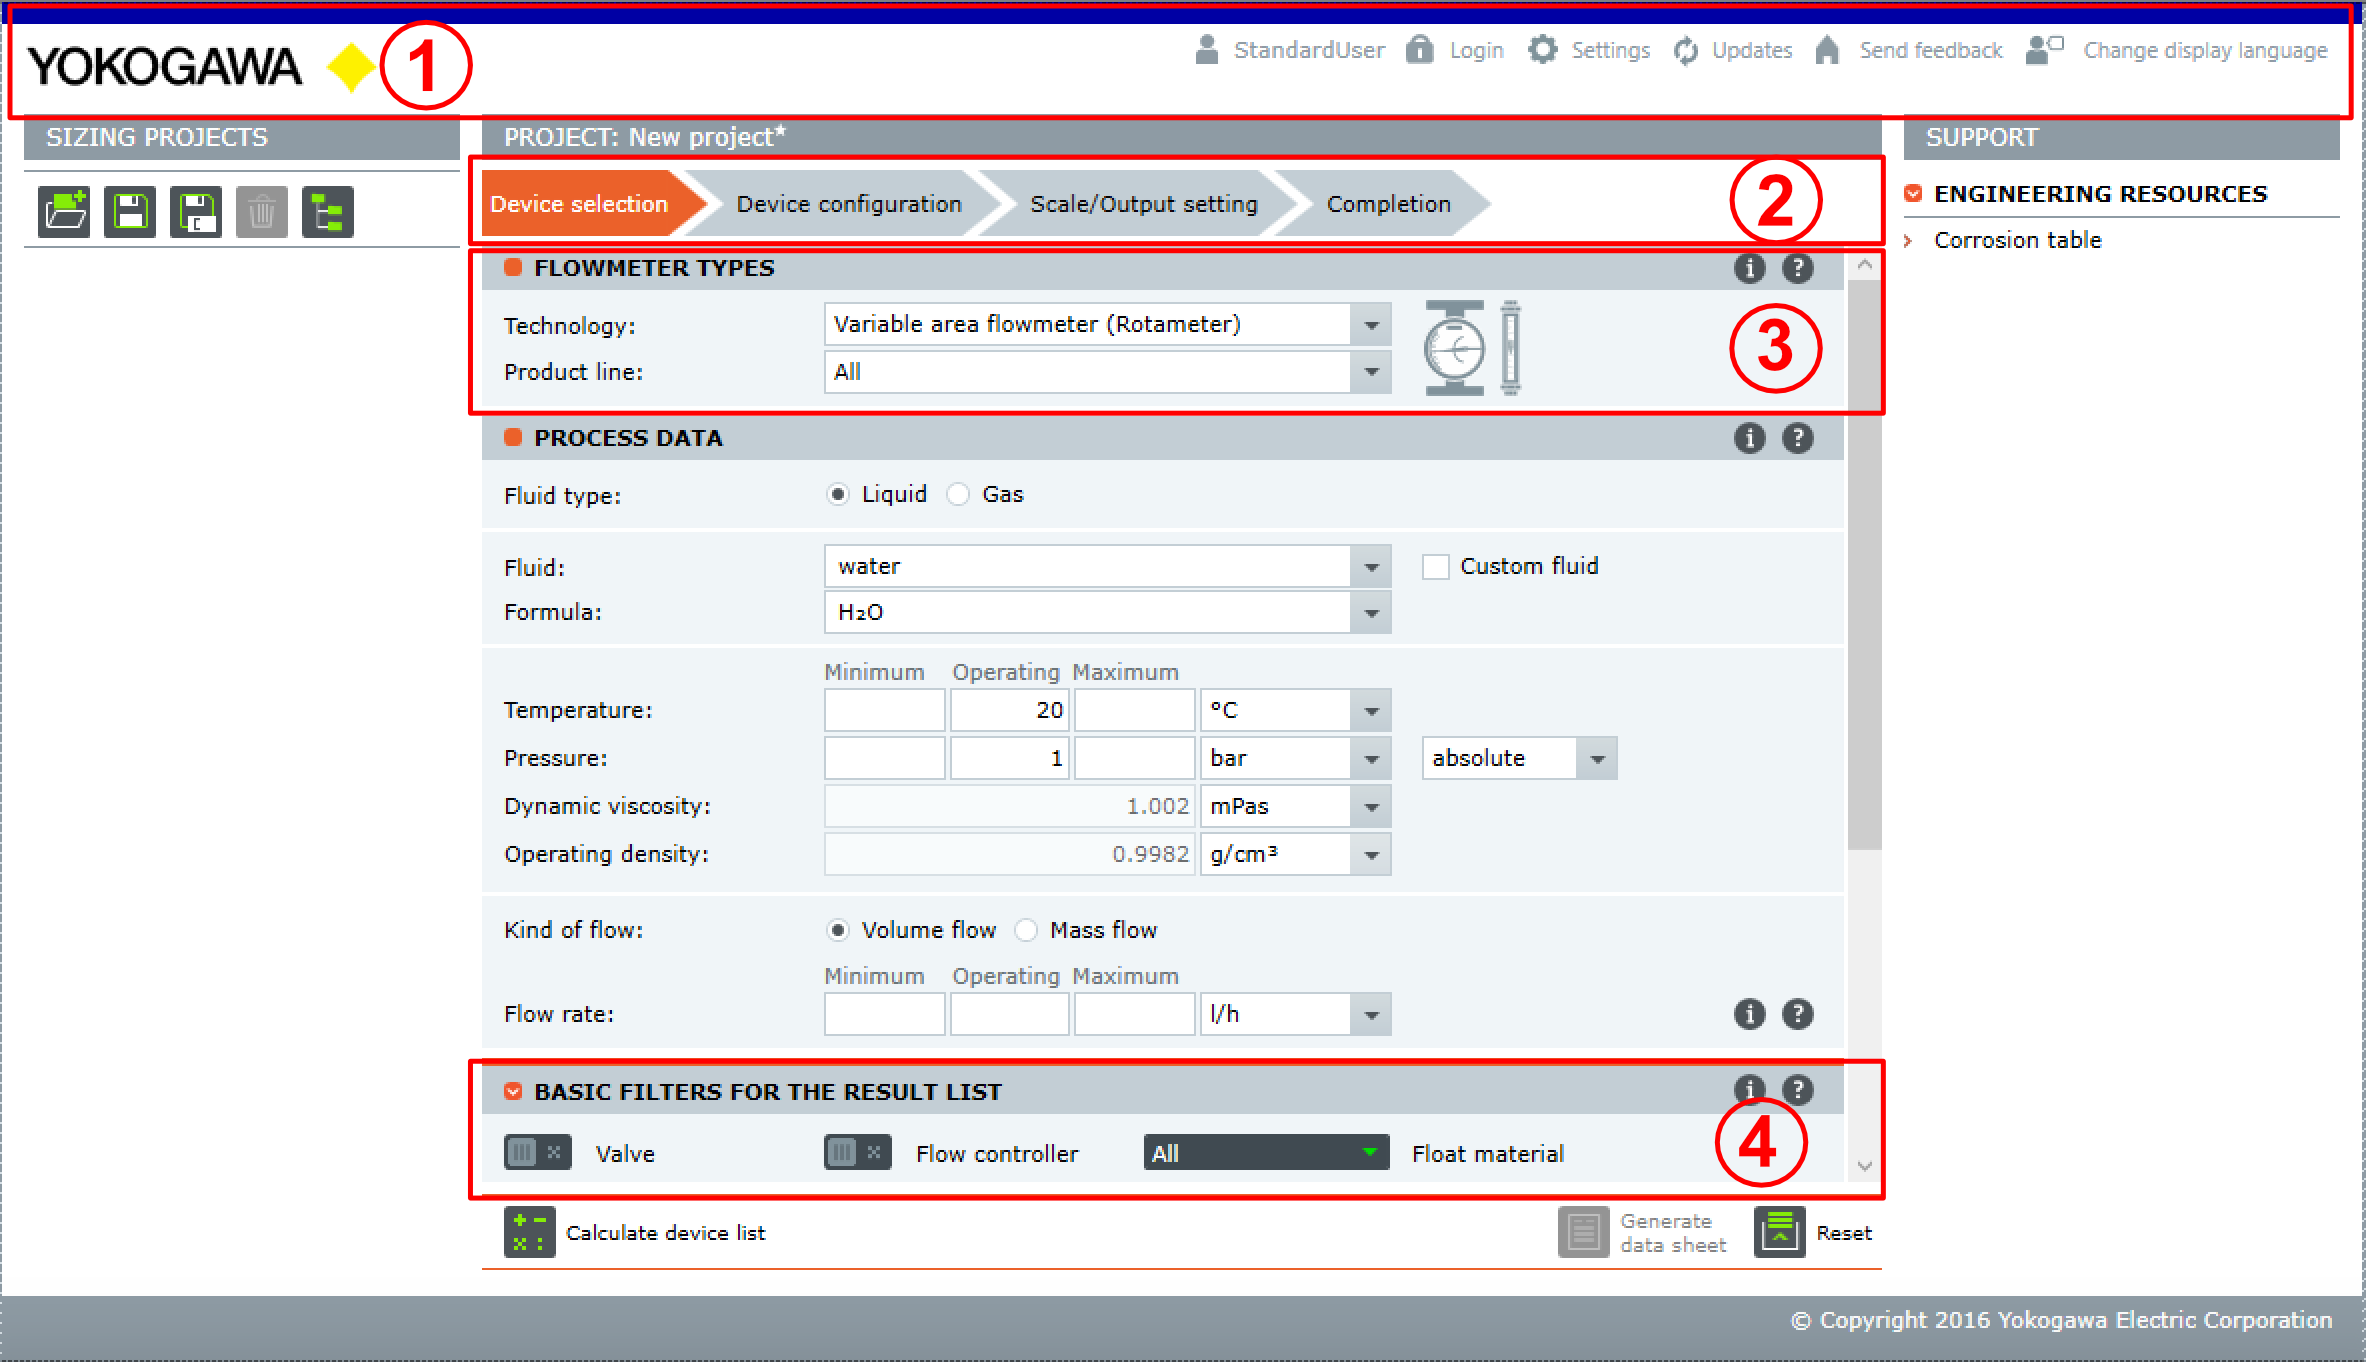
\includegraphics[width=.95\textwidth]{layout}
\caption{Identifizierung benötigter Layout-Komponenten zur Realisierung der Webanwendung}
\label{fig:layout}
\end{figure}

\subsubsection{{\larger\textcircled{\smaller[2]1}} Kopfzeile}

Die Kopfzeile zeigt dem Nutzer unter anderem an, ob er an der Applikation angemeldet ist und wenn ja unter welchem Benutzernamen. Diese Information ist ebenso für die Webanwendung relevant, da sich ein Benutzer auch an dieser anmelden muss.

\subsubsection{{\larger\textcircled{\smaller[2]2}} Navigationsassistent}

Anhand der Navigationsassistenten kann der Benutzer bestimmen, in welchem Schritt er sich bei der Gerätekonfiguration befindet und zusätzlichen bei Bedarf auch zwischen einzelnen Schritten navigieren. Die Webanwendung verfolgt mit der Bearbeitung der Filterdaten ein ähnliches Konzept, da auch diese aufgrund der Datenstruktur nur in mehreren Teilabschnitten zu bearbeiten sind. Aus diesem Grund, soll auch die Webanwendung eine ähnlich geartete Navigation realisieren.

\subsubsection{{\larger\textcircled{\smaller[2]3}} Technologie- und Produktlininenauswahl}

Anhand der bereitgestellten Dropdown-Listen schränkt der Benutzer den zu konfigurierenden Gerätetyp ein. Die getroffene Auswahl hat Auswirkungen auf die zur Verfügung stehenden Filter und muss damit auch als wichtiger Bestandteil der Webanwendung übernommen werden.

\subsubsection{{\larger\textcircled{\smaller[2]4}} Anzeige der Filtersteuerelemente}

Die Filtersteuerelemente werden auf Grundlage der in {\larger\textcircled{\smaller[2]3}} getroffenen Auswahl angezeigt. Auf dem Screenshot nicht zu sehen ist die zusätzliche Unterscheidung in Basis- und Spezialfiltern. Diese Layout-Komponente ist auch ein wesentlicher Kernbestandteil der Webanwendung, da hier die Filtersteuerelemente angezeigt werden, auf denen sich verschiedene Aktionen ausführen lassen sollen.

%
%\subsection{Benutzerführung}
%\begin{itemize}
%\item Wie funktioniert die Navigation auf der Seite mit Bezug auf das Layout
%\item Breadcrumb-Navigationshilfe erwähnen
%\item URL-Parameter steuern indirekt API (z.b. %ydm.de/filters/1 holt den Filter mit der ID 1 aus der %Datenbank und stellt Daten in einer Detailansicht dar)
%\item User Feedback Elemente und deren Einfluss auf die %Nutzerführung erläutern (Messages, Ladeanimationen etc.)
%\end{itemize}

\subsection{WYSIWYG als Gestaltungskonzept}
\label{sec:Entwurf:WYSIWYG als Gestaltungskonzept}

Dieser Abschnitt beschäftigt sich mit dem WYSIWYG-orientierten Gestaltungskonzept als ein Bestandteil der Benutzeroberflächengestaltung der Webanwendung. WYSIWYG beschreibt in seinem Kern einen Vorgang, bei dem Objekte durch den Benutzer mithilfe eines wie auch immer ausgeprägten Editors bereits so dargestellt bzw. bearbeitet werden können, wie sie dann später im \grqq{}Echteinsatz\grqq{} ebenfalls für den Benutzer der Anwendung erscheinen. Verfügbare Funktionen werden beispielsweise mit Hilfe von Steuerelementen an diesen Objekten angeboten; können dort vom Benutzer ausgewählt und auf einer Arbeitsfläche mithilfe direkter Manipulation, beispielsweise im Drag-and-Drop-Modus, verändert werden. Typische Anwendungsgebiete sind zum Beispiel WYSIWYG-Texteditoren, die es erlauben einen Text so zu formatieren, wie er später auch präsentiert wird (zum Beispiel im Druck, oder als ein Beitrag auf einer Webseite). Die angestrebte Funktionsweise der Webanwendung baut demnach auf ein sehr ähnliches Prinzip. An Stelle der eben als Beispiel genannten Texte treten komplexe Filterdaten auf, die als Filtersteuerelemente in der Benutzeroberfläche sichtbar sind. Anstatt Texte zu formatieren, soll die Ausprägung und Anordnung der Filtersteuerelemente auf einer Arbeitsfläche veränderbar sein. Dies kann aufgrund der komplexen Datenbasis natürlich nicht ausschließlich durch direkte Manipulation der Filtersteuerelemente geschehen. Es geht dabei vielmehr um den Teil der Filterdaten, welche das Aussehen und die Anordnung der Filtersteuerelemente bestimmen. Die Anordnung der Filtersteuerelemente lässt sich beispielsweise nur sinnvoll anpassen, wenn der Benutzer bei diesem Vorgang die Relation zu den umgebenden Filtersteuerelementen nicht verliert. Deshalb wird für die Webanwendung ein interaktiver Drag-and-Drop-Mechanismus konzipiert. Der Benutzer kann in der Webanwendung Filtersteuerelemente anklicken und diese frei in einem vorgegebenen Grid-System (Arbeitsfläche) verschieben. Das Ergebnis dieses Prozesses wird dann repräsentiert als Datenstruktur abgespeichert. Das bedeutet, dass die Funktionalität die für die Bearbeitung der Filtersteuerelemente realisiert wird, bereits einen - wenn auch nicht sehr ausgeprägten - WYSYWIG-Editor beschreibt.

WYSWYIG lässt sich aber außerdem noch, auf einen weiteren Aspekt des Systems übertragen. Auch wenn die Analogie etwas hinkt, lässt sich auch die Webanwendung als Ganzes als eine Art WYSIWYG-Editor betrachten. Die komplette Funktionalität der Webanwendung ist letztendlich darauf ausgerichtet Filterdaten zu bearbeiten, die zum Teil durch die angezeigten Filtersteuerelemente in der Benutzeroberfläche sichtbar gemacht werden. Durch den Export der Daten als Mittel zur Wiedernutzbarmachung in der FlowConfigurator Software ergibt sich damit ein ähnliches \ac{WYSIWYG}-Konstrukt, das bereits durch das vorangegangene Texteditor Beispiel aufgezeigt wurde. Der Vergleich ist nur deshalb nicht ganz sauber, weil aufgrund der Komplexität der zugrunde liegenden Daten nur wenige Teilbereiche der Bearbeitung tatsächlich auf direkte Manipulation von Objekten beruhen\footnote{Die direkte Manipulationen von Objekten ist ein oft genanntes Merkmal wenn von WYSIWYG-Systemen gesprochen wird, faktisch aber keine Grundvoraussetzung.}. Nichtsdestotrotz trägt auch dieser Aspekt zum Verständnis der Webanwendung als WYSIWYG-orientiertes System bei.





\chapter{Implementierung}
\label{cha:Implementierung}

In diesem Kapitel wird die Implementierung der systemtragenden Komponenten anhand von Codebeispielen erläutert. Dabei werden wichtige Gedanken und Überlegungen, die während des Entwicklungsprozesses entstanden sind, aufgegriffen und anhand der vorliegenden Implementierungen diskutiert. Ebenso wird das Ergebnis der Benutzeroberflächengestaltung und die dabei umgesetzten Konzepte beleuchtet.

\section{Server}

Die in Abschnitt \ref{sec:Entwurf:Server} vorgestellten Kernkomponenten der Serverarchitektur werden in diesem Abschnitt im Detail beleuchtet und dabei vor allem wichtige Implementierungen hinsichtlich der an die Webanwendung gestellten Anforderungen erläutert.

\subsection{Model}

In Abschnitt \ref{sec:Entwurf:Server} wurden Models bereits als Bestandteile der Datenzugriffsschicht eingeführt. Models sind dabei Klassen die Tabellen einer relationalen Datenbank hinsichtlich ihrer Eigenschaften, Schemata und Beziehungen beschreiben. Modelklassen erlauben es, zur Laufzeit der Anwendung objektorientierte Datenmodelle mit Hilfe eines Mappers in eine relationale Datenbank abzulegen. Die Funktion des Mappers übernimmt im Kontext dieser Implementierung das \acf{ORM} Framework Eloquent. Eloquent ist ein Bestandteil des Laravel PHP Frameworks, auf dem die gesamte serverseitige Implementierung aufbaut. Die Modelklassen werden gemäß den in Abschnitt \ref{sec:Analyse:Server} gestellten technologischen Anforderungen nach dem Database-First-Prinzip vollständig generiert. Als Generator wurde dabei die Bibliothek \emph{laravel-model-generator} verwendet, die die Funktionen des Eloquent Framework um die benötigte Funktionalität erweitert. Das Ergebnis einer solchen generierten Modelklasse wird in Listing \ref{prog:model} als Programmcode dargestellt.

\begin{program}[H]
% place caption consistently either at the top or bottom:
\begin{PhpCode}
<?php namespace App\Models;

use Illuminate\Database\Eloquent\Model;

class FilterFilterGroup extends Model {

    protected $primaryKey = 'filterGroupID';
    protected $table = 'Filter_FilterGroup';
    protected $fillable = ['shortName', 'displayName', 'infoTooltip', 'helpTooltip', 'initiallyCollapsed', 'displaySequence'];


    public function translation() {
        return $this->belongsTo(\App\Models\CommonTranslateWordId::class, 	'displayName', 'wordID');
    }

    public function filterFilters() {
        return $this->hasMany(\App\Models\FilterFilter::class,'filterGroupID','filterGroupID');
    }
}
\end{PhpCode}
\captionof{lstlisting}{Beispiel einer generierten Modelklasse}
\label{prog:model}
\end{program}

Im oberen Abschnitt der Klasse finden sich Merkmale und Eigenschaften, die das Schema der zugehörigen Datenbanktabelle beschreiben. Die dargestellten Funktionen beschreiben hingegen die Beziehung zu verknüpften Tabellen. Diese Beziehungen werden mithilfe von Funktionen modelliert, die vom Eloquent-Framework bereitgestellt werden. Jede Modelklasse leitet von einer Basismodelklasse ab. Diese Basismodelklasse implementiert wiederum ein Interface, mit dessen Hilfe die Datenbank angesprochen werden kann. Der Zugriff auf die Datenbank erfolgt dabei Model zentriert. Modelklassen bilden damit das Rückgrat der Serverimplementierung, indem sie es erlauben Daten aus Datenbankabfragen als Objekt zu kapseln, das im weiteren Verlauf im Kontext einer objektorientierten Implementierung genutzt werden kann.

\subsection{Controller}

Controller wurden in Abschnitt \ref{sec:Entwurf:Server} als Implementierung der Ressourcen des entwickelten RESTful Webservice. Controller implementieren Models um auf Grundlage der HTTP-Methoden, die auf einer Ressource aufgerufen werden können, konkrete Datenbankabfragen zu realisieren. Ein Controller beinhaltet bis auf wenige Ausnahmen immer genau vier Methoden: Lesen, Speichern, Löschen und Aktualisieren von Ressourcen. Um die Integration mit den Models zu erklären, wird in Listing \ref{prog:controller} als Beispiel eine eher komplexere Update-Methode dargestellt.

\begin{program}[H]
% place caption consistently either at the top or bottom:
\begin{PhpCode}
   public function update(FilterRequest $request, $id)
    {
        DB::beginTransaction();

        try {
            $input = $request->json()->all();
            $filter = Filter::with('translation.en')->findOrFail($id);
            $group = FilterGroup::findOrFail($input['group']['id']);
            $type = FilterType::findOrFail($input['type']['id']);
            $productGroup = ProductGroup::findOrFail($input['productGroup']['id']);

            $filter->translation->en->first()->word = $input['name'];
            $filter->shortName = $input['shortName'];
            $filter->filterDisplaySequence = $input['sequence'];

            $filter->group()->associate($group);
            $filter->type()->associate($type);
            $filter->productGroup()->associate($productGroup);

            if ($filter->push()) {
                DB::commit();
                return $this->item($filter, new FilterTransformer());
            }
        } catch (\Exception $e) {
            DB::rollback();
            throw $e;
        }
    }
\end{PhpCode}
\captionof{lstlisting}{Beispiel einer Update-Methode aus einem API-Controller}
\label{prog:controller}
\end{program}

Die dargestellte Methode realisiert die Aktualisierung einer Filter-Ressource. Das über die Schnittstelle gesendete, zu aktualisierende Filterobjekt, wird als Request-Objekt gekapselt und neben der ID an die Update-Methode übergeben. Die Update-Methode implementiert die entsprechenden Modelklassen um den Aktualisierungsvorgang zu realisieren. Eine Besonderheit dabei ist, dass Operationen, die Daten in die Datenbank schreiben, immer in einem Transaktionsblock definiert sind. Das hat den Vorteil, dass es quasi ausgeschlossen ist, aufgrund von fehlerhaften Abfragen einen inkonsistenten Datenbankzustand zu provozieren. Wenn auf Datenbankebene ein Fehler auftritt, wird die laufende Transaktion abgebrochen und der ursprüngliche Zustand der Datenbank wiederhergestellt.

In Programmzeile 6 bis 10 wird anhand von Modelklassen das zu aktualisierende Filterobjekt und ebenfalls die zu aktualisierenden Relationen geladen. Konnten die Relationen gefunden bzw. geladen werden, werden diese mit dem Filterobjekt verknüpft (Programmzeile 16-18) und anschließend das aktualisierte Filterobjekte persistiert (Programmzeile 20). Eine Besonderheit ergibt sich aus der in Programmzeile 22 definierten Rückgabefunktion, die einen sogenannten Transformer aufruft und damit die Überleitung zu den in Abschnitt \ref{sec:imp:Transformer} betrachteten Transformern herstellt.

\subsection{Transformer}
\label{sec:imp:Transformer}

Transformer wurden in Abschnitt \ref{sec:Entwurf:Server} als Komponenten zur Homogenisierung und Standardisierung von Rohdaten eingeführt. Die im vorherigen Abschnitt beschriebenen Controller-Methoden definieren alle einen Rückgabewert. Diese Rückgabewerte sind immer Repräsentationen von Ressourcen im Kontext der jeweiligen aufgerufenen Methode und werden immer durch einen Transformer realisiert. Das bedeutet, das Transformer die Repräsentation einer Ressource hinsichtlich des Inhalts und Formats bestimmen. Eine Transformer-Klasse wird in der Regel immer von genau einem Controller implementiert. Sie haben die Aufgabe, die aus den Abfragen der Modelklassen resultierenden Rohdaten in ein für den RESTful Webservice geeignet Format zu überführen. Dieser Vorgang wird in Listing
\ref{prog:transformer} exemplarisch dargestellt. Um logisch an das gegebene Beispiel aus Abbildung \ref{prog:controller} anzuschließen wurde ein Ausschnitt aus der korrespondierende FilterTransformer-Klasse gewählt. 

\begin{program}[H]
% place caption consistently either at the top or bottom:
\begin{PhpCode}
public function transform(Filter $filter)
    {
        return [
            'id' => (int) $filter->filterID,
            'name' => $filter->translation->en->first()->word,
            'shortName' => $filter->shortName,
            'sequence' => (int) $filter->filterDisplaySequence,
            'spaceLeft' => (int) $filter->filterSpaceLeftInPixel,
            'spaceRight' => (int) $filter->filterSpaceRightInPixel
        ];
    }
\end{PhpCode}
\captionof{lstlisting}{Beispiel einer Transform-Methode aus einer Transformer-Klasse}
\label{prog:transformer}
\end{program}

Die Methode \emph{transform()} wird in diesem Beispiel mit einem Modelobjekt vom Typ Filter aufgerufen. Anhand von Zugriffen, die über die Modelklasse realisiert werden, kann so ein Rückgabeobjekt mit beliebigen Inhalt und Format modelliert werden. Dabei geht es aber nicht nur um simple Anpassung von Bezeichnern, wie zum Beispiel in Programmzeile 4 geschehen\footnote{An dieser Stelle wird, die aus der Datenbank kommende \emph{filterID}, auf das Feld \emph{id} gemappt. Das Mapping von ID's geschieht in jedem Transformator nach demselben Schema und beschreibt einen Teil der Datenhomogenisierung.}, sondern auch um Mapping-Funktionen\footnote{Als Mapping wird der Prozess bezeichnet, der Datenelemente zwischen unterschiedlichen Datenmodellen abbildet.} über Relationen hinweg. In Programmzeile 5 erfolgt ein solches relationales Mapping, indem die englische Übersetzung des Anzeigenamens des übergebenden Filterobjekts aus der Translation-Tabelle geladen und auf das Feld \emph{name} gemappt wird. Zusammenfassend lassen sich also zwei Kernaufgaben der Transformatoren herausstellen:

\begin{itemize}
\item Die Konvertierung von Rohdaten, in ein für die Schnittstelle geeignetes Format
\item Die Realisierung von benötigten Abhängigkeiten über das nachladen von in Beziehung stehenden Datenobjekten oder -feldern.
\end{itemize}

\subsection{Router}

Der Router wurde in Abschnitt \ref{sec:Entwurf:Server} als die Komponente beschrieben, die die Schnittstelle des entwickelten Webservice realisiert. Der Router realisiert die Schnittstellenspezifikation, in dem er alle verfügbaren Endpunkte und die jeweils aufrufbaren HTTP-Methoden implementiert. Wird ein Endpunkt von einem Client aufgerufen, werden die ankommenden Daten automatisch durch das Laravel Framework in ein Request-Objekt geschrieben. Dieses Request-Objekt enthält neben allen Informationen, die im HTTP-Header und Body übertragen werden, auch Metainformationen über das verwendete Datenformat. Außerdem stellt ein Request-Objekt unter anderem auch Helferfunktionen zur Verfügung, um die Daten aus dem HTTP Message Body zu parsen. Die Schnittstelle implementiert als Datenformat \acf{JSON}, ist aber so flexibel gestaltet, dass serverseitig auch eine problemlose Umstellung auf \ac{XML} erfolgen kann. Der Einsatz von \ac{JSON} als Datenformat macht im Kontext eines auf Javascript basierenden Webfrontend aber in jedem Fall Sinn, da clientseitig JSON-Objekte ohne weiteres Zutun in Javascript-Objekte umgewandelt werden können. 

Der Router implementiert außerdem sogenannte Middlewares, die bestimmte Funktionen auf einer festgelegten Gruppe von Endpunkten ausführen. Über eine Authentifizierungsmiddleware erfolgt beispielsweise die Absicherung der Schnittstelle. Das in Abbildung \ref{fig:authentification} dargestellte Sequenzdiagramm beschreibt Auszugsweise den Vorgang der Authentifizierung.
\begin{figure}[H]
\centering
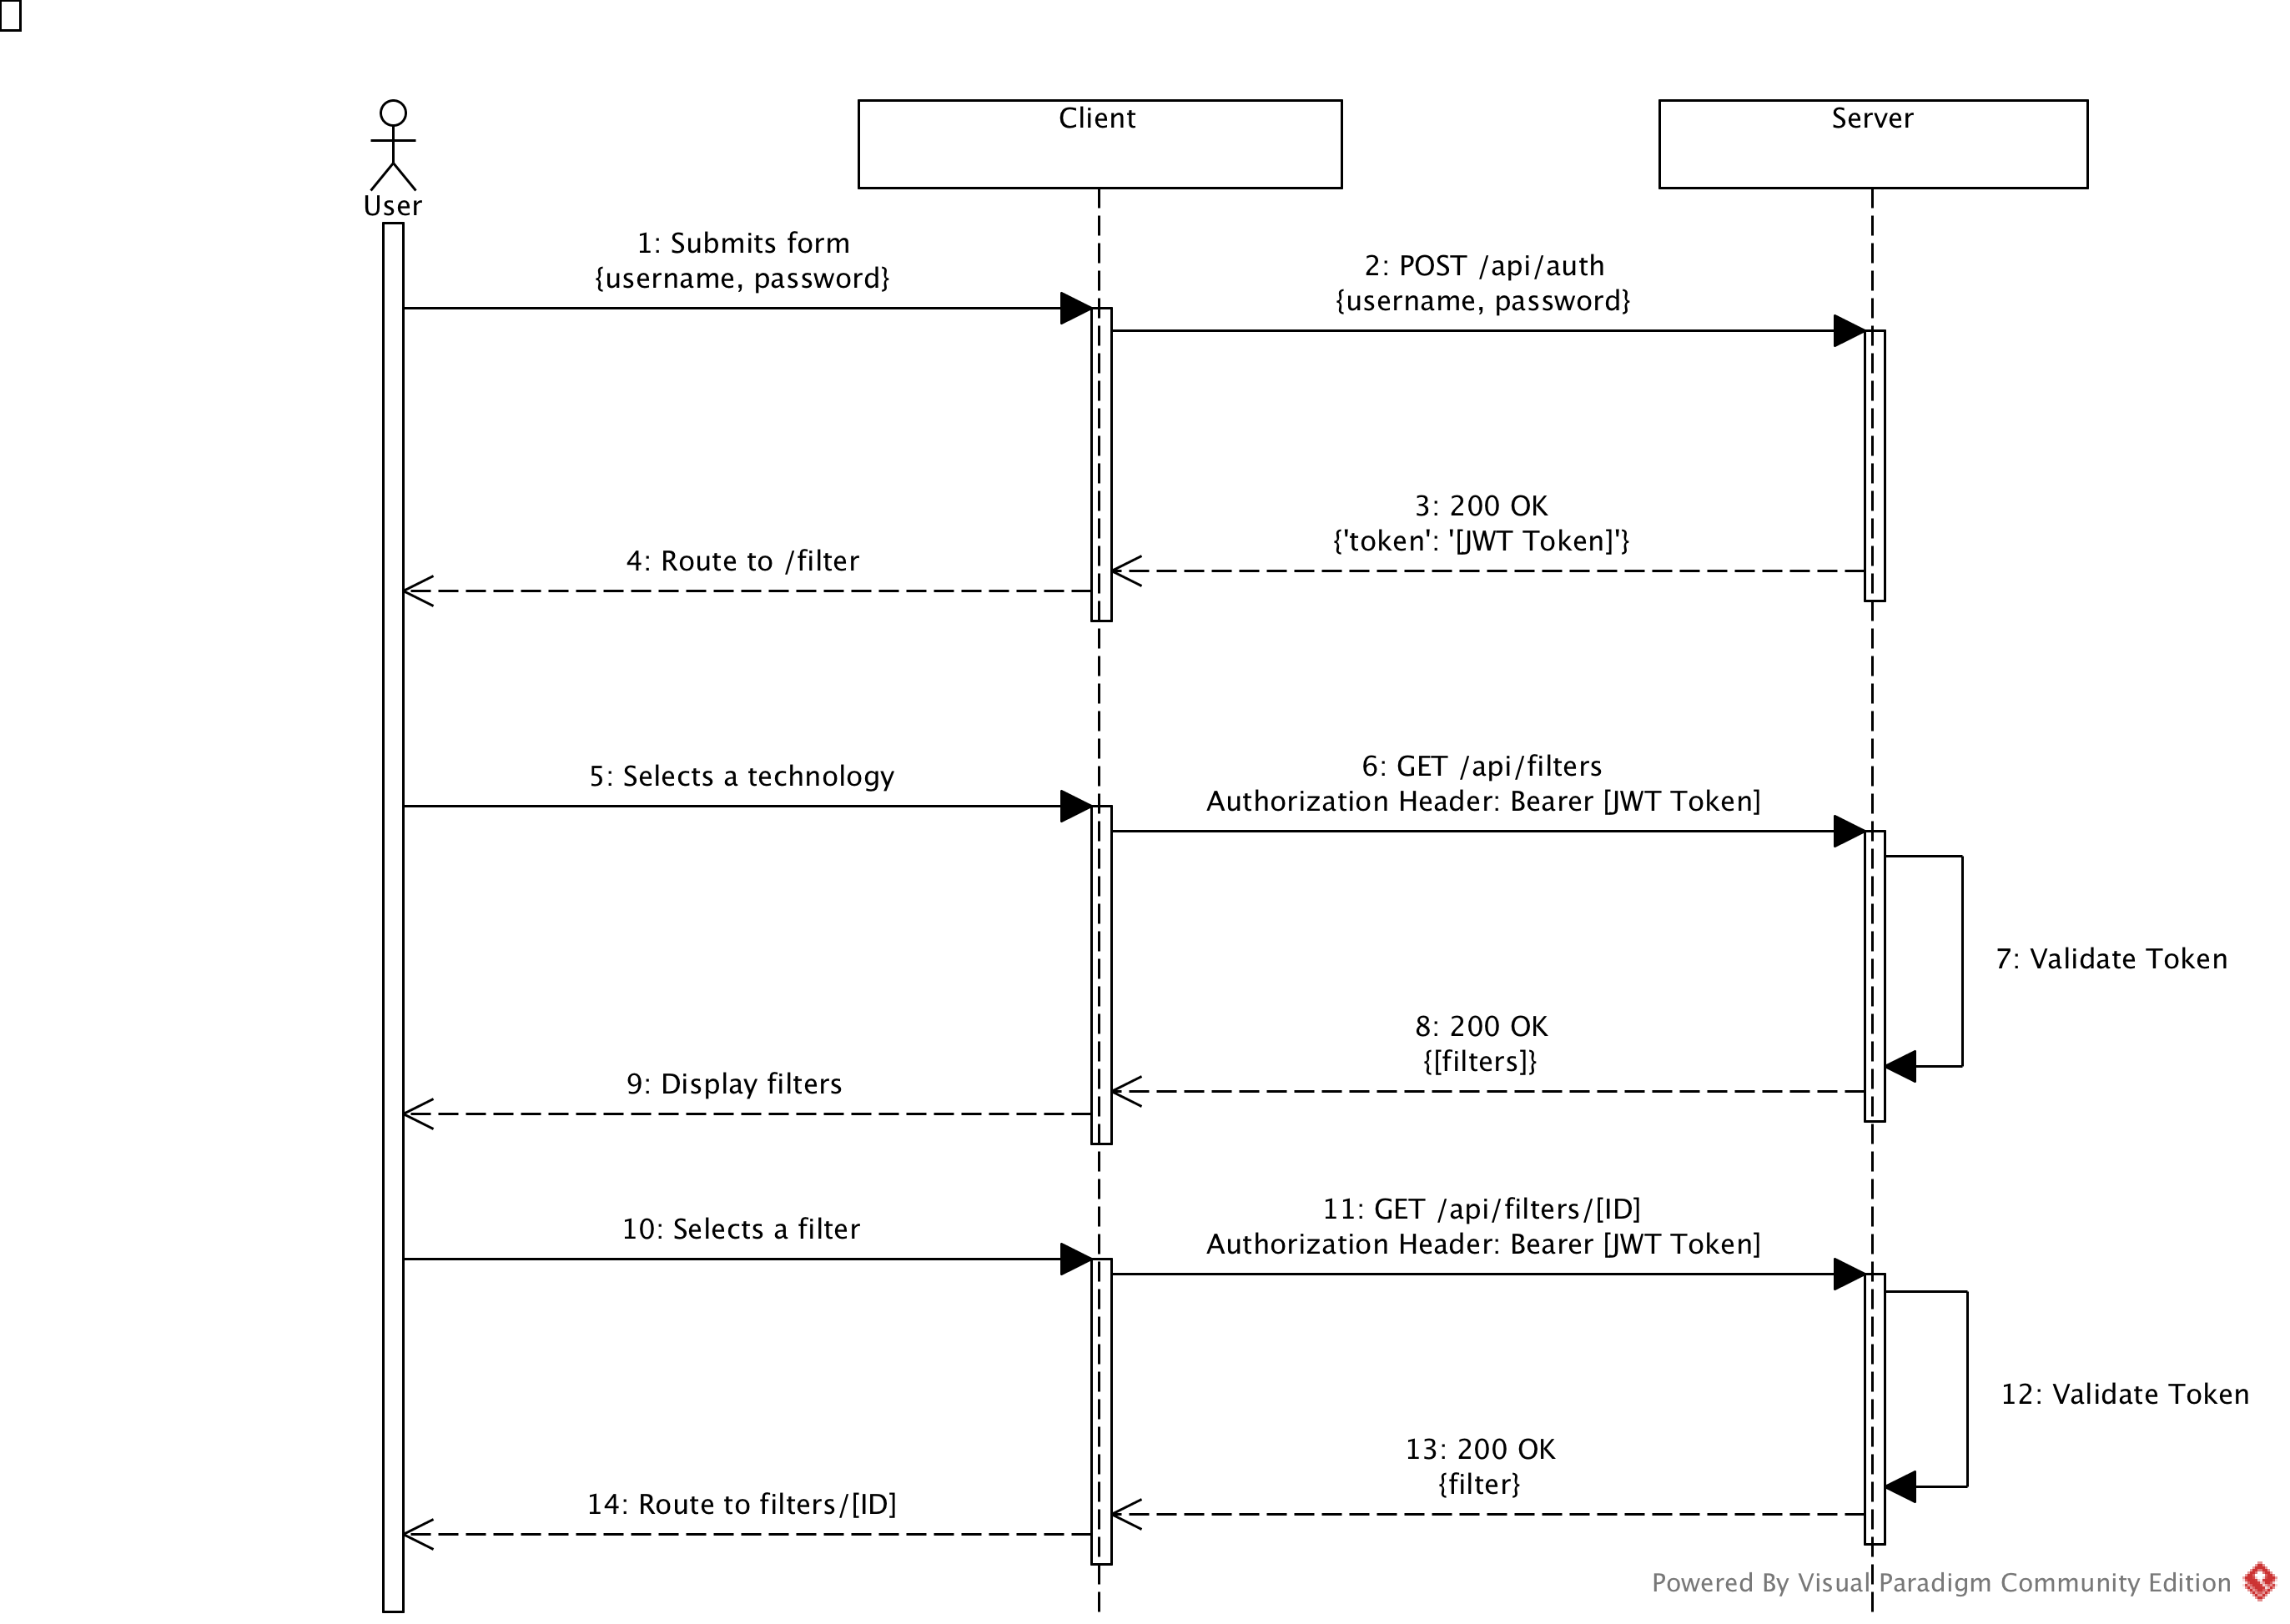
\includegraphics[width=1.0\textwidth]{authentification} %{CS0031}
\caption{Tokenbasierte Authentifizierung}
\label{fig:authentification}
\end{figure}
Die Authentifizierung am Server erfolgt über die in Abschnitt \ref{sec:ROA:Sicherheit} vorgestellten tokenbasierten Authentifizierung. Ein Benutzer muss sich nach der in Abschnitt \ref{sec:Funktionale Anforderungen} gestellten Anforderung \glqq{}\emph{Anmelden}\grqq{} an der Webanwendung anmelden, um deren Funktionalität nutzen zu können. Die Anmeldung erfolgt über einen Benutzernamen und ein Passwort. Die eingegebenen Anmeldedaten werden serverseitig mit einer User-Tabelle abgeglichen. Sind die Anmeldedaten korrekt, wird von der Authentifizierungsmiddleware ein Token generiert, der mit einem geheimen Schlüssel signiert wird. Dieser Token wird als Antwort zurück an den Client geschickt, der das Token in einem sogenannten Cookie ablegt. Durch die Ablage des Tokens in einem Browser-Cookie, kann der Benutzer zwischenzeitlich auch seinen Browser schließen und bei erneutem Besuch der Webanwendung den selben Token wiederverwenden; der Benutzer muss sich also nicht noch einmal neu Anmelden, solange der Token noch gültig ist. In dem dargestellten Sequenzdiagramm werden beispielhaft weitere Interaktionen des Benutzer und Aufrufe des Clients dargestellt. Dadurch soll ausgedrückt werden, dass der Token ab der Anmeldung in jedem HTTP-Request als Teil des Header mitgesendet wird. Auch die Validierung des Tokens erfolgt bei jedem Aufruf einer geschützten Ressource. Anhand dieser Implementierung wird eine sichere und zustandslose Art der Authentifizierung realisiert.

\section{Client}

Die Frontend-Komponente der Webanwendung wurde mit dem Javascript-Framework \mbox{AngularJS} entwickelt. In Abschnitt \ref{sec:Entwurf:Client} wurde bereits ausgeführt, dass \mbox{AngularJS} ein klassisches MVC-Architekturmuster als \ac{SPA} realisiert. Schwerpunkt der nachfolgenden Abschnitte bildet die Betrachtung der einzelnen Frontend-Komponenten und ihrer Rollen im Kontext der Gesamtanwendung. Außerdem wird das Ergebnis der Benutzeroberflächenimplementierung anhand ausgewählter Aspekte beleuchtet.

\subsection{Model}

Das Model enthält die darzustellenden Daten und ist von Präsentation und Steuerung unabhängig. Models werden im Kontext von AngularJS typischerweise an einer Variable \emph{\$scope} definiert. Dies kann sowohl innerhalb eines Controllers als auch direkt im View über eine sogenannte Direktive erfolgen. Direktiven realisieren Funktionen, die das Vokabular von HTML erweitern. Mittels Direktiven können neue HTML-Tags und Attribute erstellt oder durch bestimmte Funktionalität erweitert werden. Über ein sogenanntes Two-Way-Databinding, das von AngularJS realisiert wird, können Models sowohl im Controller als auch im View verändert werden. Die jeweils andere Komponente wird dann über die Änderung benachrichtigt und kann sich aktualisieren. Die Implementierung von Models beschränkt sich im Falle der Webanwendung auf einfache Variablen die am \emph{\$scope} gespeichert werden. Das sind vor allem Daten, die über den Webservice geladen und in Form von Javascript-Objekten nutzbar gemacht werden. Die Definition solcher \emph{\$scope} Variablen erfolgt im Falle der Webanwendung fast ausschließlich in den jeweiligen Controllern, um eine bessere Übersicht zu gewährleisten. Die Models der Webanwendung realisieren dabei im wesentlichen folgende Funktionen:

\begin{itemize}
\item Generierung der datengetriebenen Filtersteuerelemente, indem die Modeldaten an entsprechende Direktiven übergeben werden. Diese Direktiven realisieren dann die konkrete Ausprägung des Filtersteuerelements (Dropdown-Liste oder Schalter)
\item Schnittstelle zwischen Dateneingabemasken (Formularen) und Controller-Logik, indem Models über Direktiven an Formularelemente gebunden werden.
\end{itemize}

\subsection{Repository}
\label{sec:imp:Respository}

Das Repository bildet das Gegenstück, der auf der serverseite realisierten Router-Komponente. Das Repository kapselt alle Endpunkte der Schnittstelle, die das Webfrontend für die Erfüllung seiner Aufgaben benötigt. Der Zugriff auf die Schnittstelle wurde mit Hilfe der Javascript-Bibliothek \emph{Restangular} realisiert. Restangular simplifiziert den Zugriff auf eine REST-konforme Schnittstelle wesentlich. So ist es zum Beispiel möglich eine Ressource Filter mit minimalen Aufwand durch den folgenden Aufruf anzusteuern.
\begin{JsCode}[numbers=none]
     getFilter: function(id, params) {
                    return Restangular.one('filters', id).get(params);
                },
\end{JsCode}
In diesem Beispiel wird aus dem in der Methode \emph{one()} übergebenen URI-Bestandteilen der Zugriff auf die Schnittstelle vollautomatisch durch Restangular realisiert. Das zurückgegebene Objekt beinhaltet neben den erwarteten Filterdaten auch Methoden zum Manipulieren des Objekts. So kann das Filterobjekt zum Beispiel im Verlauf der Anwendung modifiziert werden und anschließend einfach eine Methode \emph{save()} direkt auf dem Objekt aufgerufen werden. Anhand der an dem Objekt gespeicherten Metadaten, kann Restangular den Zugriff auf die Ressource zum Speichern der Daten ableiten und vollautomatisch realisieren. Ein manuelles Implementieren von Funktionen zum Speichern, Löschen oder Aktualisieren von Ressourcen entfällt damit clientseitig vollständig. 

\subsection{Controller}

Im Gegensatz zu den serverseitigen Controllern, haben die Controller auf der Clientseite keinen klar abgegrenzten Aufgabenbereich. Geht man nach den Empfehlungen von AngularJS sollten Controller lediglich die Bindung von Datenobjekten an die \emph{\$scope} Variable realisieren. Die Controller implementieren diesen Sachverhalt, indem sie über ein Repository mittels eines \ac{AJAX}-Aufrufs den Webservice ansprechen und das Ergebnis an den besagten \emph{\$scope} binden. Außerdem implementieren Controller auch die Geschäftslogik der Clientseite, die zum Beispiel für die Modifizierung von Datenstrukturen oder anderen aufgabenrelevanten Sachverhalten benötigt wird. Einer dieser Sachverhalte im Kontext der in Abschnitt \ref{sec:Funktionale Anforderungen} ermittelten funktionalen Anforderungen ist von besonderer Wichtigkeit und wird daher nachfolgend im Detail betrachtet. Die funktionale Anforderung \glqq{}\emph{Filter anzeigen}\grqq{} aus Abschnitt \ref{sec:Funktionale Anforderungen} lautet: 
\begin{quote}
Filtersteuerelemente müssen dem Benutzer angezeigt werden. Die Anwendung generiert die Filtersteuerelemente anhand der Filterdaten und orientiert sich dabei am Layout des FlowConfigurator. Die Anzeige muss zusätzlich Schaltflächen, für die auf die Filter anwendbaren Operationen enthalten (Bearbeiten, Löschen, Erstellen).
\end{quote}
Diese Anforderung impliziert eine besondere Herausforderung an die datengestützte Generierung der Filtersteuerelemente im Webfrontend. Die in der Datenbasis vorliegenden layoutspezifischen Daten, die die Anordnung der Filtersteuerelemente beschreiben, basieren auf einem Fließlayout. Das bedeutet, dass in der FlowConfigurator Software Filtersteuerelemente einfach nacheinander in einen dafür vorgesehenen Container geladen werden (siehe Abbildung \ref{fig:layout}) und dabei benötigte Abstände zwischen Filtersteuerelementen über Pixelangaben realisiert werden. Diese Pixelangaben sind Teil der layoutspezifischen Daten und werden direkt in der Filtertabelle gespeichert. Aufgrund der in Abschnitt \ref{sec:Analyse:Nichtfuntionale Anforderungen} aufgestellten Anforderung an die Portabilität, die unter anderem besagt, dass die Webanwendung möglichst auch auf kleinen Bildschirmen korrekt dargestellt werden soll, wurde sich für die Darstellung der Filtersteuerelemente in einem Grid-Layout entschieden. Dieses Grid-System wurde mit Hilfe des Frontend Frameworks Bootstrap realisiert und bietet den Vorteil das Spalten und Zeilen definiert werden können, die je nach Bildschirmgröße korrekt umbrechen und damit eine solide Basis eines responsiven Layouts bilden. Die Herausforderung liegt nun darin begründet, aus den Daten eines Fließlayouts, ein Grid-Layout zu generieren, dass die Filtersteuerelemente exakt so anzeigt werden, wie in der FlowConfigurator Software. Zu diesem Zweck wurden die Filterdaten eingehend analysiert und anhand von Oberflächentests ermittelt, nach welchem Muster die Filtersteuerelemente im FlowConfigurator angezeigt werden. Dabei konnte festgestellt werden, dass die FlowConfigurator Software stehts ein zwei- oder dreispaltiges Layout simuliert. Anhand dieser Erkenntnis wurden Regeln formuliert, die die Grundlage generischer Algorithmen bilden, welche anhand der gegebenen Filterdaten im Webfrontend ermitteln können, ob die Filtersteuerelemente in einem zwei- oder dreispaltigen Layout angezeigt werden sollen. Zusammenfassend lässt sich der Prozess der datengetriebenen Generierung der Filterelemente damit durch folgende Punkte:

\begin{enumerate}
\item Filterdaten werden über die Schnittstelle geladen
\item Ein Algorithmus bestimmt ob ein zwei- oder dreispaltiges Layout für die Darstellung der Filtersteuerelemente verwendet werden soll
\item Die Filtersteuerelemente werden auf Basis des ermittelten Layouts generiert und Abstände zwischen Elementen die größer als eine Spalte sind durch Platzhalterelemente ersetzt
\end{enumerate}
Das Ergebnis dieser Implementierung wird im Abschnitt \ref{sec:imp:Benutzeroberfläche} dargestellt.

\subsection{Router}

Der Router ist die Kernkomponente des Clients und definiert alle \ac{URL}'s die innerhalb des Client-Frontend aufgerufen werden können. In Abschnitt \ref{sec:Entwurf:Client} wurde bereits erörtert, dass sich der Router aus sogenannten States zusammensetzt, welche das Zusammenspiel der einzelnen Client-Komponenten orchestrieren. Anhand des in Listing dargestellten Programmcodes wird der Aufbau eines solchen States beispielhaft erläutert.
\begin{program}[H]
% place caption consistently either at the top or bottom:
\begin{JsCode}
$stateProvider
.state('app.filters.edit', {
    url: '/filters/{fId:int}',
    ncyBreadcrumb: {
        label: function ($stateParams) {
            return $stateParams.fId
        }
    },
    views: {
        'content@app': {
            templateUrl: 'app/app/filter/edit/edit.html',
            controller: 'FilterEditCtrl'
        }
    },
    resolve: {
        filter: function (Repository, $stateParams) {
            return Repository.getFilter($stateParams.fId).then(function (res) {
                return res.data.plain();
            })
        },
        types: function (Repository) {
            return Repository.getFilterTypes().then(function (res) {
                return res.data.plain();
            })
        },
        groups: function (Repository) {
            return Repository.getFilterGroups().then(function (res) {
                return res.data.plain();
            })
        },
        productGroups: function (Repository) {
            return Repository.getProductGroups().then(function (res) {
                return res.data.plain();
            })
        },
    }
})
\end{JsCode}
\captionof{lstlisting}{Beispiel eines Router-States}
\label{prog:router}
\end{program}
Ein State ist ein Mittel zur Beschreibung von Vorgängen, die beim Aufruf einer bestimmten Route erfolgen. Der dargestellte State besteht aus vier Bestandteilen, die nachfolgend getrennt voneinander betrachtet werden.

\subsubsection{URL}

Die Funktion \emph{url} bestimmt die \ac{URL}, die aufgerufen werden muss um den State zu \glqq{}aktivieren\grqq{}. Dieser Parameter kann auch dynamische Bestandteile enthalten. Zum Beispiel wird in Programmzeile 3 ein Parameter als Bestandteil der \ac{URL} definiert. Diese Parameter lassen sich ebenfalls typisieren. Im vorliegenden Beispiel wird der State nur aktiviert, wenn der Parameter ein Integer-Wert ist. Die Parameter werden durch ui-router ausgelesen und können im weiteren Verlauf der Anwendung für verschiedene Zwecke genutzt werden.

\subsubsection{Views}

Die Funktion \emph{views} gibt an, welche HTML-Templates beim Aufruf eines States geladen und wo auf der Webseite sie angezeigt werden sollen. Ein Template kann dabei mit einem Controller verknüpft werden. Für rein statische Templates kann die Verknüpfung mit einem Controller aber auch entfallen. Bezogen auf den Beispielcode wird ein Template zur Bearbeitung von Filterdaten geladen, das mit einem korrespondierenden Controller verknüpft wird.

\subsubsection{Resolve}

Der Parameter resolve ist ein Mittel um Abhängigkeiten vor dem Darstellen eines HTML-Templates und vor dem Aufruf eines möglichen verknüpften Controllers aufzulösen. Im Falle des Beispiels wird die Resolve-Funktion in Programmzeile 15-36 für das Laden von Daten über den Webservice benutzt. Zu diesem Zweck wird das Respository implementiert. Eine Besonderheit stellt der Aufruf in Programmzeile 17 dar. Hier wird aufbauend auf dem Beispiel aus Abschnitt \ref{sec:imp:Respository} ein Filter mit einer bestimmten ID geladen. Die ID ist dabei der dynamische Bestandteil aus der vorher definierten \ac{URL}. Dieses Konzept wird in vielen States der Webanwendung angewandt und erlaubt es damit sogar indirekt das Verhalten der Webanwendung in Bezug auf die Schnittstelle des Webservice zu steuern. Beispielsweise könnte ein Benutzer, wenn er die ID eines bestimmten Filterobjektes wüsste, diese direkt an die \ac{URL} anhängen und auf die entsprechende Seite für die Bearbeitung genau dieses Filters gelangen.

\subsubsection{ncyBreadcrumb}

Die Funktion ncyBreadcrumb ist eine eigene Erweiterung der State-Funktionalität, um eine sogenannte Breadcrumb-Navigation zu realisieren. Eine Breadcrumb-Navigation stellt die Navigationshierarchie dar, mit Hilfe derer ein Benutzer erfährt, wo genau er sich innerhalb der Webanwendung befindet. Diese Implementierung ist ein direkter Lösungsansatz um die in Abschnitt \ref{sec:Analyse:Identifizierung von Layout-Komponenten} identifizierte benötigte Layout-Komponente Nummer 2 zu realisieren.

\subsection{Benutzeroberfläche}
\label{sec:imp:Benutzeroberfläche}

Die Benutzeroberfläche setzt sich aus einzelnen Views (HTML-Templates) zusammen, deren Komposition über die Router-Komponente gesteuert wird. Für die Realisierung der Benutzeroberfläche wurde das Frontend Framework Bootstrap eingesetzt. Die in Abschnitt \ref{sec:Funktionale Anforderungen} gestellten funktionalen Anforderungen dienen maßgeblich als Orientierung für die benötigten und zu gestaltenden HTML-Templates. Das Ergebnis dieses Prozesses wird als Screenshot der Benutzeroberfläche in Abbildung \ref{fig:userinterface} dargestellt.
\begin{figure}[H]
\centering
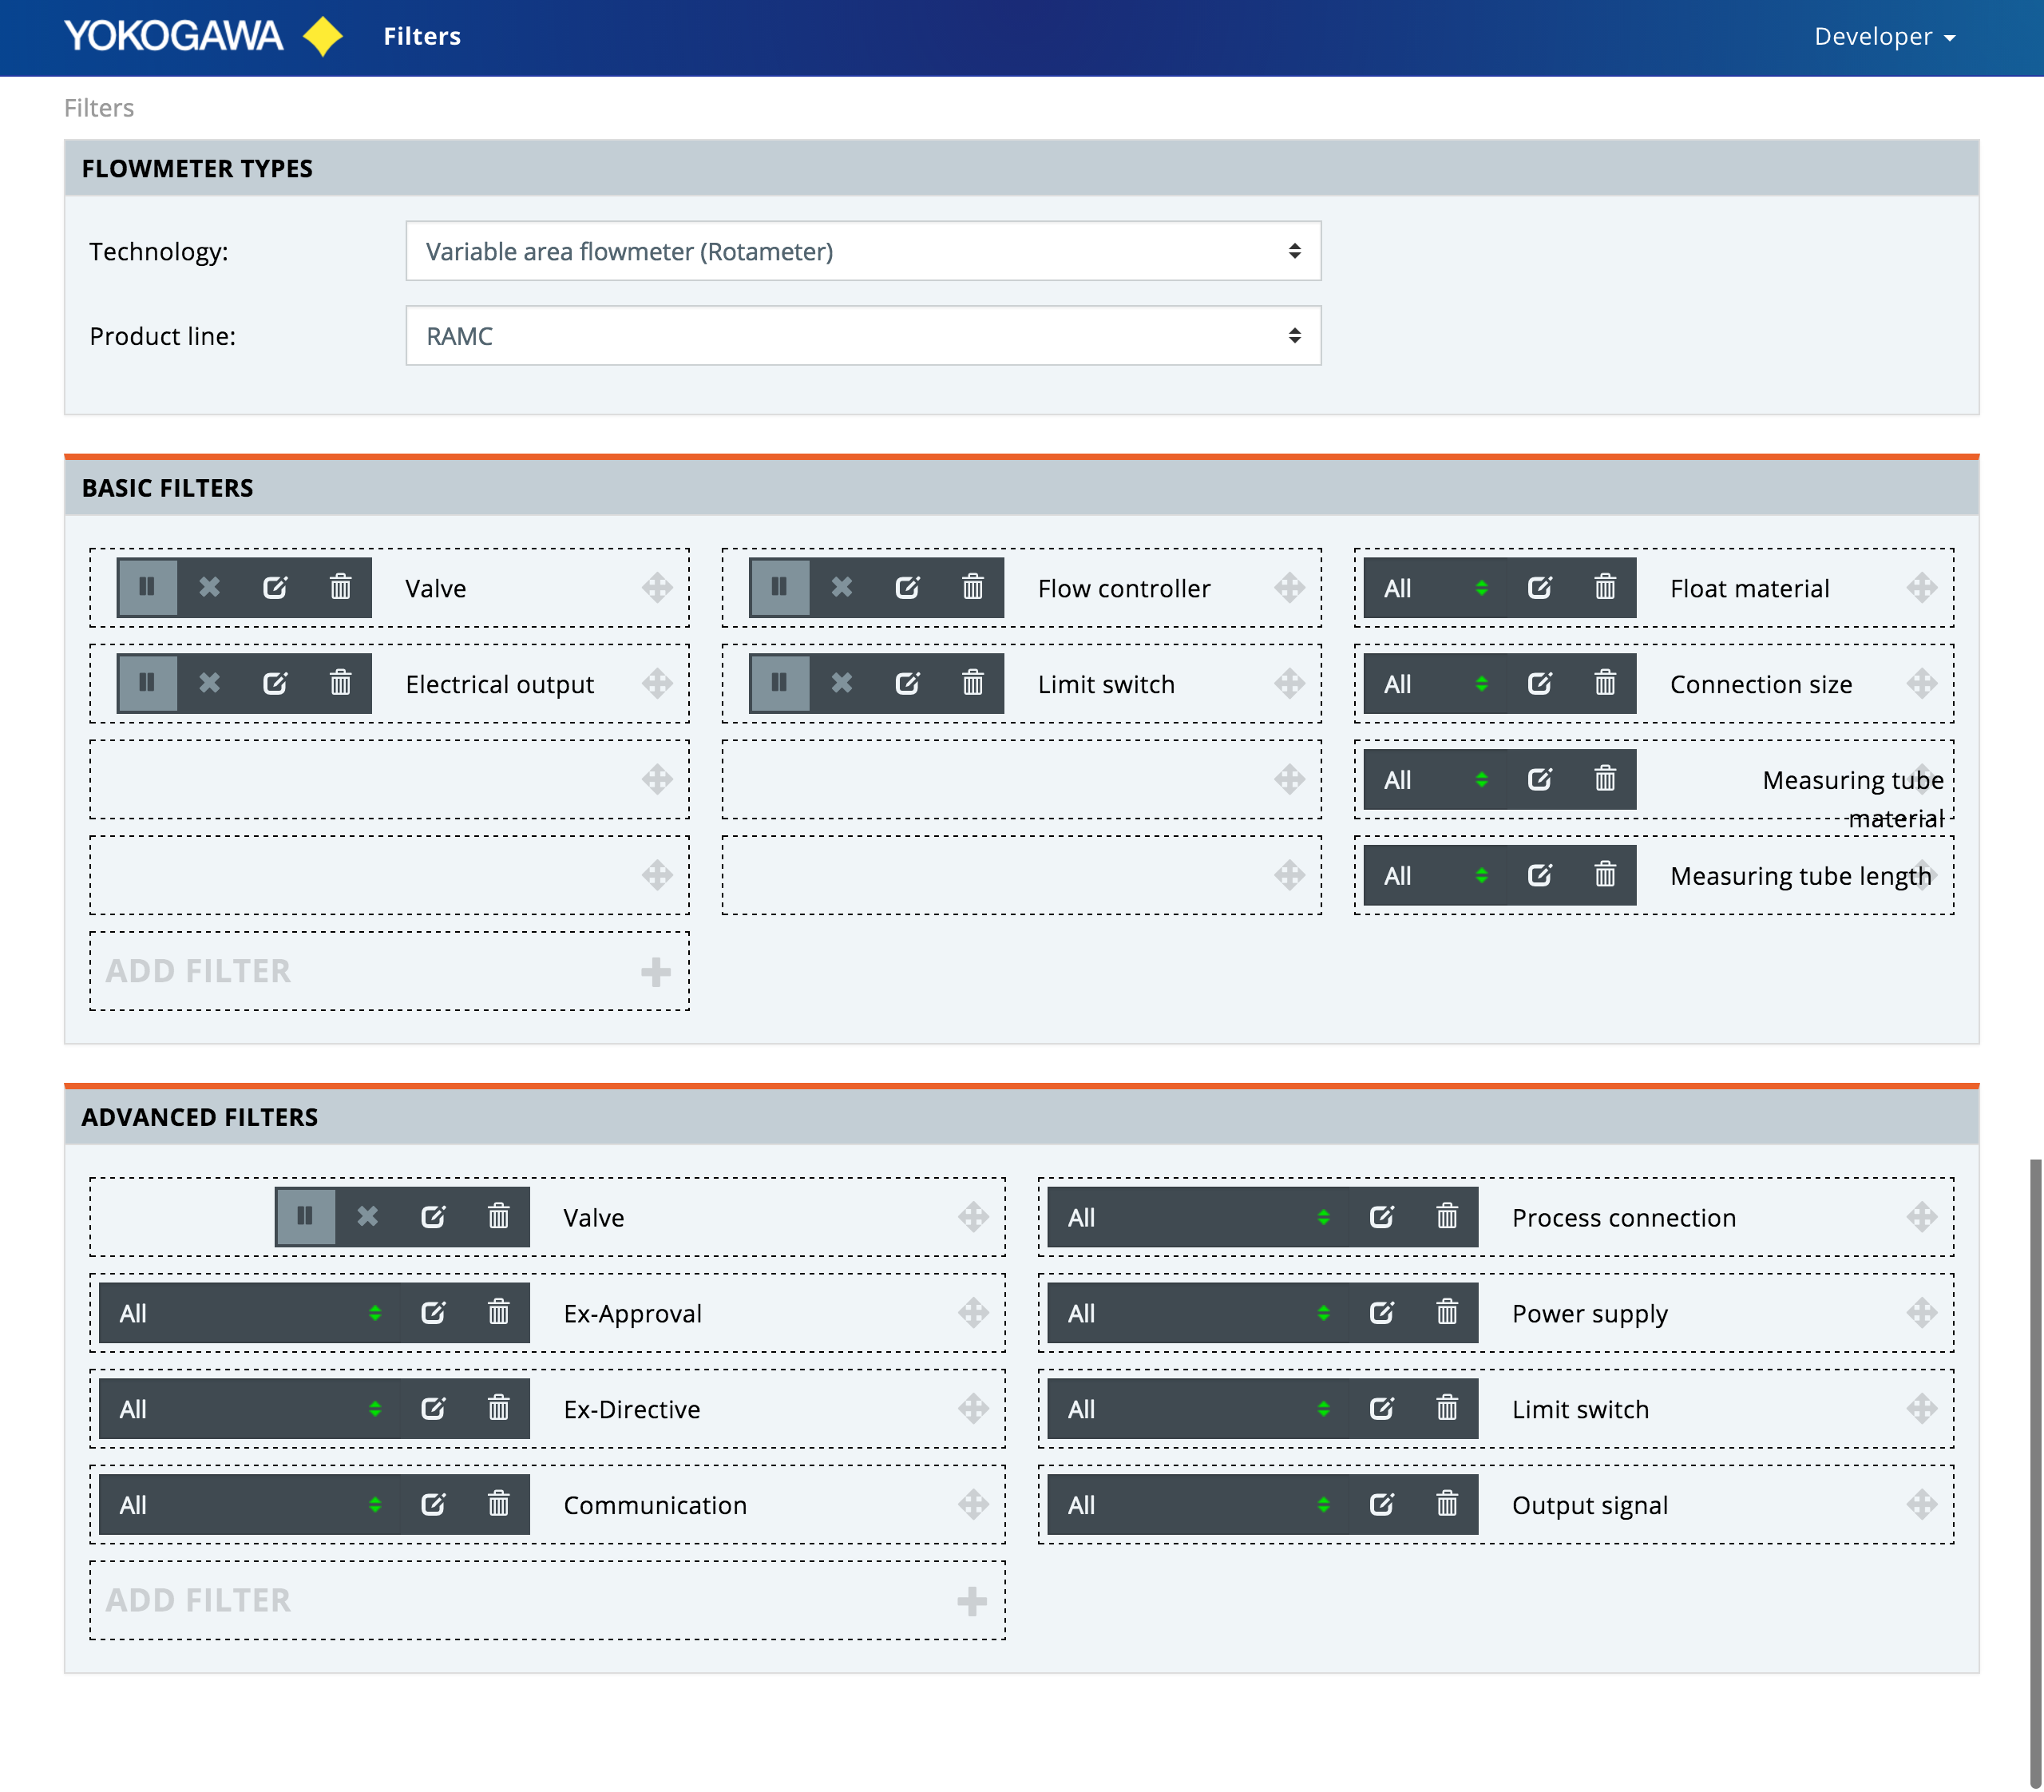
\includegraphics[width=1.0\textwidth]{ydm-index} %{CS0031}
\caption{Screenshot der Filterübersicht der Webanwendung.}
\label{fig:userinterface}
\end{figure}
Nachfolgend werden die realisierten View-Komponenten, aus denen sich die Benutzeroberfläche zusammensetzt, mit den gestellten Anforderungen abgeglichen und wichtige Konzepte und Gedanken zur Gestaltung diskutiert. Hauptanforderung an die Benutzeroberfläche war die inhaltliche und gestalterische Nähe zur FlowConfigurator Software. Dabei ging es keinesfalls darum eine exakte Kopie der Benutzeroberfläche der FlowConfigurator Software zu entwickeln, sondern durch den bedachten Einsatz von übergreifenden Gestaltungsmerkmalen und stilistischen Mitteln einen ähnlichen \glqq{}Look and Feel\grqq{} zu erzeugen. Die in Abschnitt \ref{sec:Analyse:Identifizierung von Layout-Komponenten} identifizieren und zu übernehmende Layout-Komponenten wurden umgesetzt und an die Anforderungen einer modernen Webanwendung angepasst. Das Hauptaugenmerk lag dabei auf der Gestaltung der Layoutkomponenten für die Anzeige der Filtersteuerelemente. Wie auf dem Screenshot in Abbildung \ref{fig:userinterface} zu erkennen ist, wurden die Filtersteuerelemente im Vergleich zur FlowConfigurator Software vergrößert, um eine bessere Bearbeitbarkeit zu gewährleisten. Die Steuerelemente wurden außerdem durch Buttons erweitert, die es erlauben Funktionen, auf Grundlage der in Abschnitt \ref{sec:Funktionale Anforderungen} ermittelten Kernanforderungen, direkt auf dem jeweiligen Steuerelement auszuführen. Das Aussehen der Steuerelemente wurde mittels \ac{CSS} an das Erscheinungsbild im FlowConfigurator angeglichen. Nur durch den Einsatz von \ac{CSS} konnten sogar normale HTML-Checkboxen als Schalter nach der Vorlage im FlowConfigurator realisiert werden.

Die Filtersteuerelemente werden vollständig datengetrieben in einem Grid-Layout generiert. Dieses Grid-Layout realisiert außerdem, einen Drag-and-Drop Funktionalität zum Verschieben der Filtersteuerelemente auf Basis der in Abschnitt \ref{sec:Entwurf:WYSIWYG als Gestaltungskonzept} erfolgten Vorbetrachtung. Die Drag-and-Drop Funktionalität wird in der Benutzeroberfläche durch die Umrandung der Filtersteuerelemente und einem entsprechenden Icon gekennzeichnet. Der Benutzer kann die Steuerelemente frei in dem dafür vorgesehenen Grid-Layout, das durch Platzhalterelemente ergänzt wird, verschieben. Das Verschieben der Steuerelemente funktioniert zudem auch über Filtergruppen hinweg. So ist es zum Beispiel möglich, einen Basisfilter in den Container der erweiterten Filter zu verschieben. Die entsprechenden Datenanpassungen werden im Hintergrund vorgenommen und müssen anschließend vom Benutzer über einen Dialog bestätigt werden.  

Neben der auf WYSIWYG basierenden Implementierung der Bearbeitung von Filtersteuerelement mit Hilfe direkter Manipulation, wurden außerdem HTML-Templates für die Bearbeitung der Geschäftsdaten entworfen. In Abbildung \ref{fig:editpage} wird solch eine Seite als Screenshot dargestellt.
\begin{figure}[H]
\centering
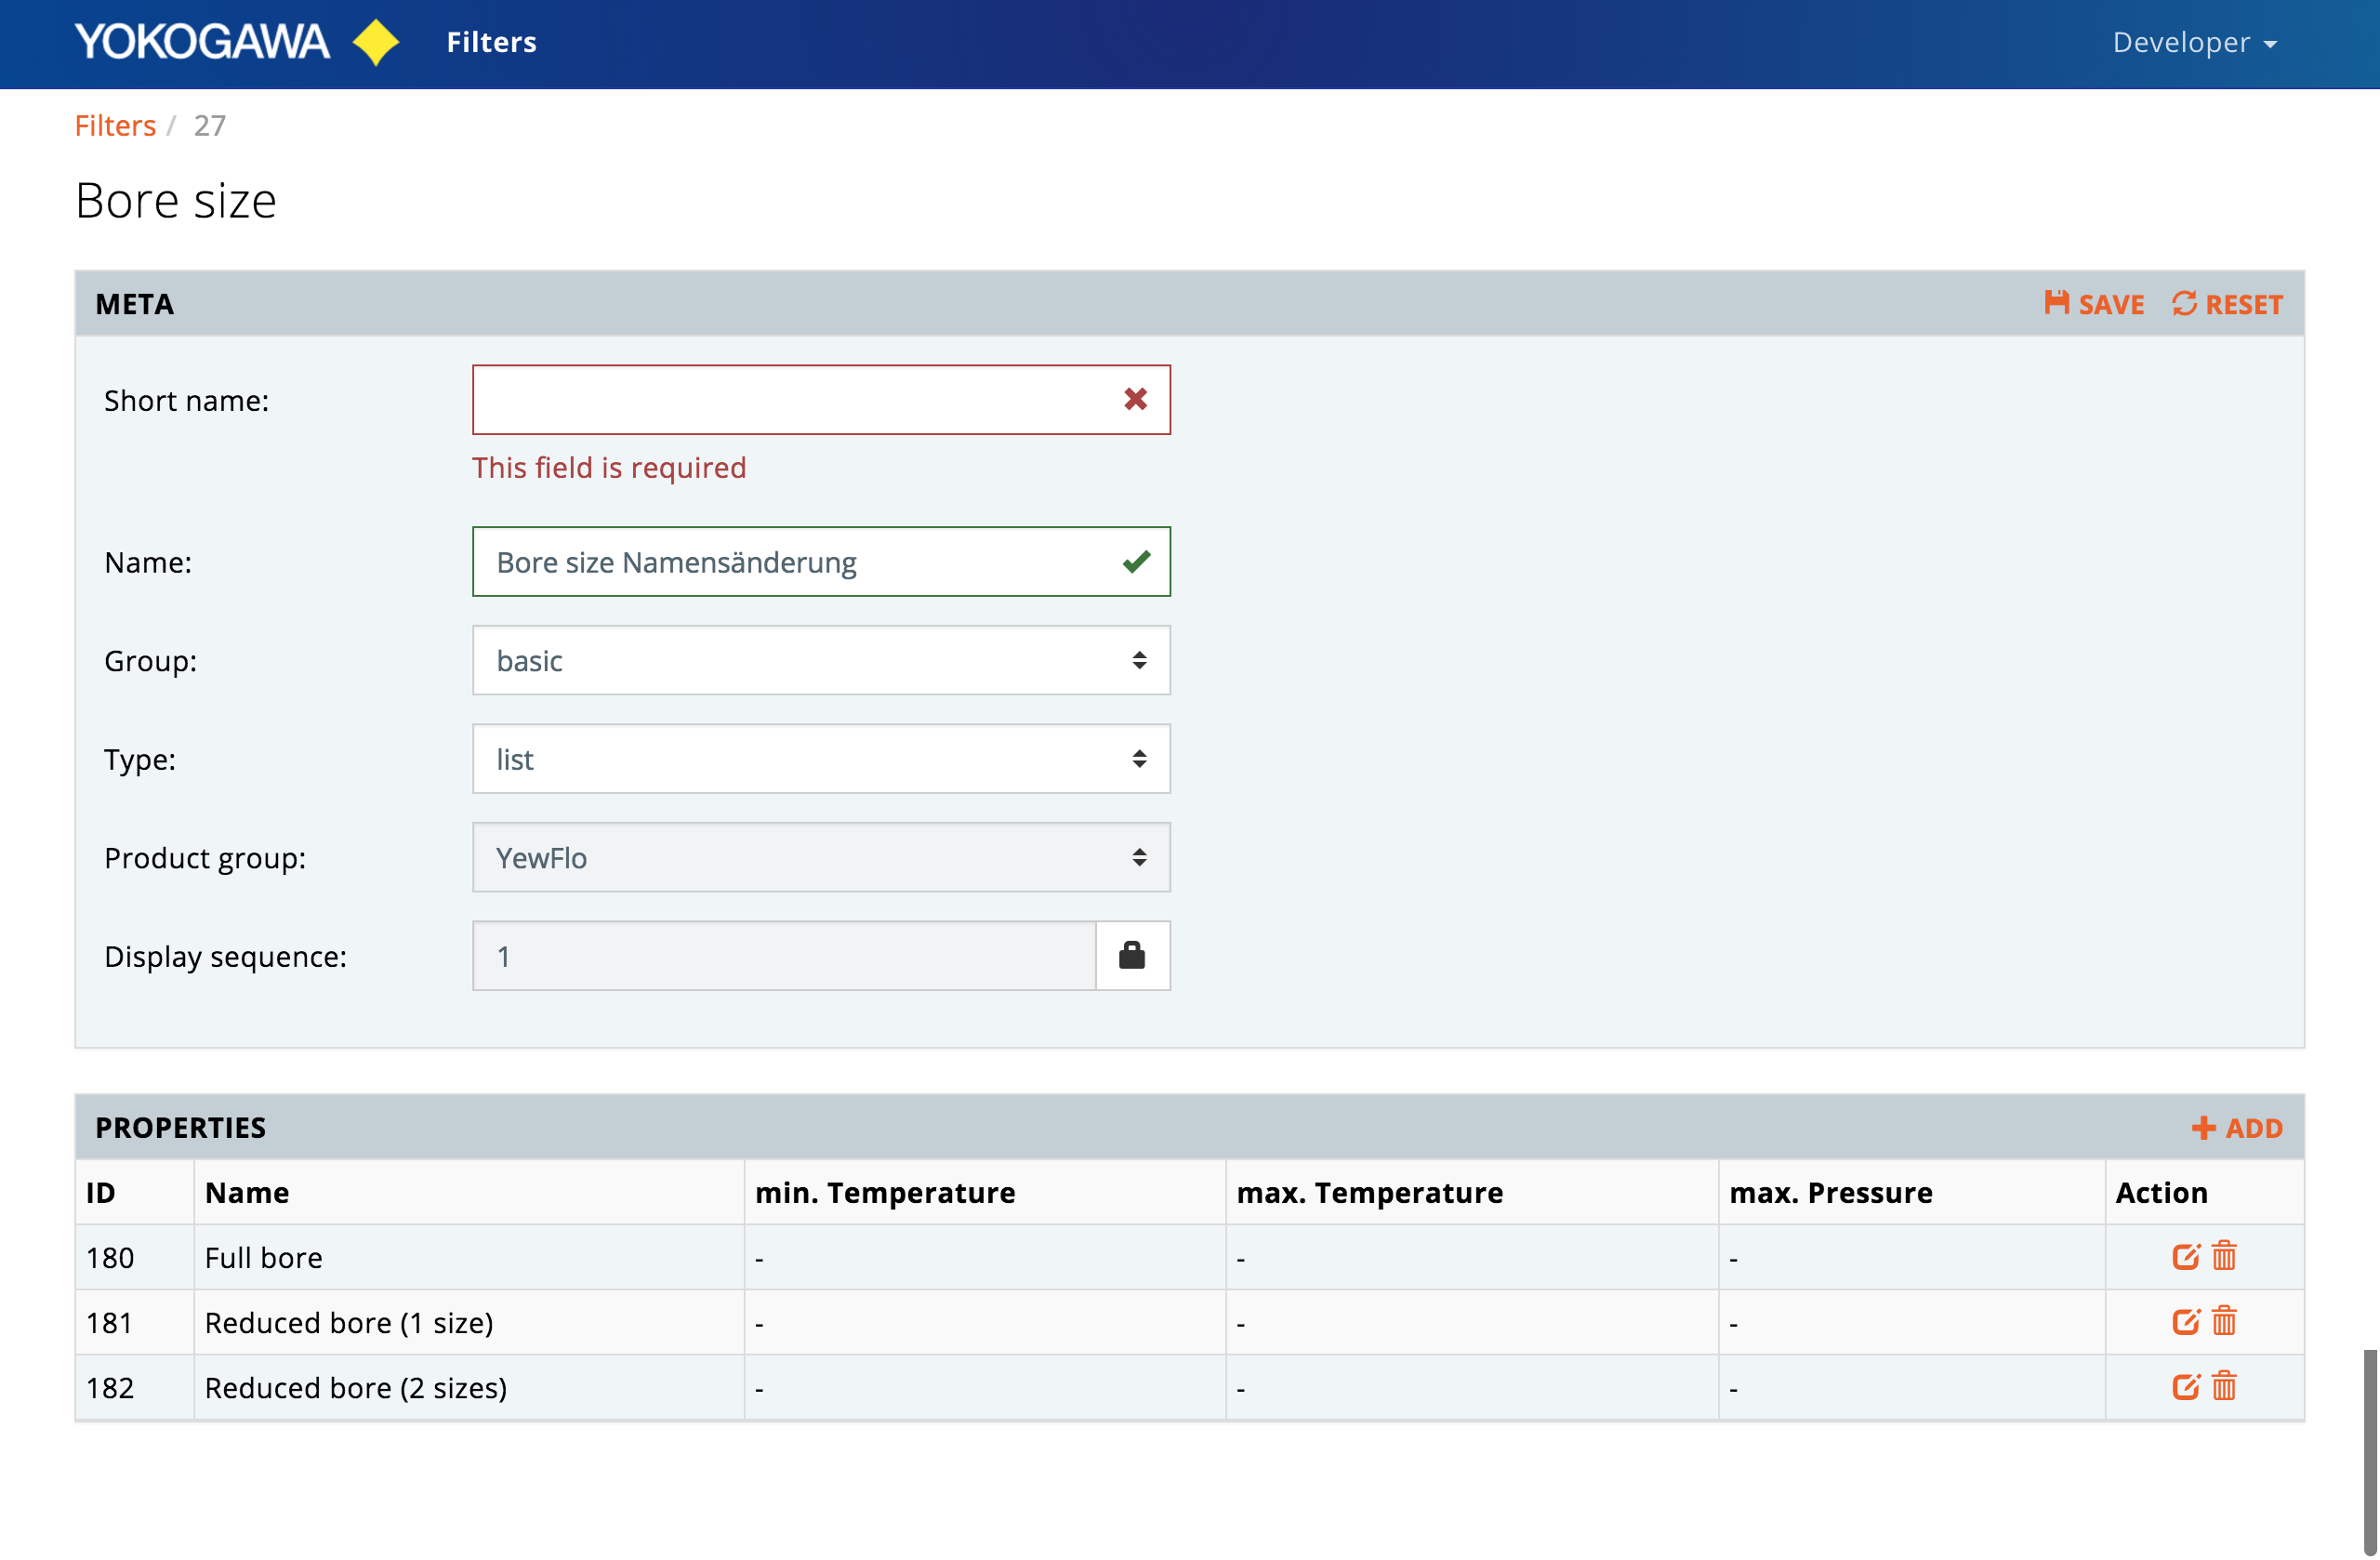
\includegraphics[width=1.0\textwidth]{ydm-edit} %{CS0031}
\caption{Screenshot einer Seite zum Bearbeiten von Filterdaten.}
\label{fig:editpage}
\end{figure}
Der Screenshot zeigt eine Seite zum Bearbeiten der Filterkerndaten. Diese Seite wird erreicht, indem der Benutzer auf den entsprechenden Bearbeiten-Button eines Filtersteuerelements klickt. Für die Gestaltung dieser Art von Seite, wurde sich an keiner konkreten Vorlage aus der FlowConfigurator Software orientiert. Es wurden aber dieselben übergreifenden Gestaltungsmerkmale und Stilmittel eingesetzt, die überall in der Webanwendung verwendet werden, um ein konsistentes Erscheinungsbild zu gewährleisten. Die dargestellte Seite zum Bearbeiten der Filterdaten realisiert Dateneingabemasken für die an einem Filterobjekt bearbeitbaren Daten. Außerdem wird über eine Tabelle die Abhängigkeit zu Properties hergestellt. Auf diesen lassen sich ebenfalls über nebenstehende Icons entsprechende Aktionen, auf Grundlage der gestellten funktionalen Anforderungen, ausführen. Als Beispiel wird in dem gezeigten Screenshot auch eine Validierung der eingegebenen Daten dargestellt, die in der gesamten Webanwendung in gleicher Art und Weise implementiert ist. Über die unter dem Header befindliche Breadcrumb-Navigation, erkennt der Benutzer, in welchem Schritt der Filterbearbeitung er sich gerade befindet. Entscheidet sich der Benutzer beispielsweise eine Property zu bearbeiten, erweitert sich diese Breadcrumb-Navigation und stellt zusätzlich die Möglichkeit bereit, zwischen einzelnen Bearbeitungsschritten zu navigieren. Die für die Erfüllung der restlichen funktionalen Anforderungen zu implementierenden Datenbearbeitungsseiten bauen alle auf ein ähnliches Layout auf und sind schrittweise über die bereitgestellten Kontextfunktionen erreichbar.

\chapter{Test}
\label{cha:Test}
In diesem Kapitel werden die Anforderungen an die Webanwendung anhand eines Integrationstests überprüft. Zu diesem Zweck wird ein Testszenario beschrieben und der Versuchsaufbau erläutert. Das zu erwartende Ergebnis wird anschließend mit dem tatsächlich eingetretenen Resultat abgeglichen.

\section{Vorgehensweise}
\subsection{Verfahren}

Aus zeitlichen Gründen konnten keine softwaregestützten Tests implementiert werden. Stattdessen wurden die in Abschnitt \ref{sec:Funktionale Anforderungen} gestellten funktionalen Anforderungen mit Hilfe eines manuell durchgeführten Integrationstests überprüft. Ein Integrationstest kennzeichnet sich durch eine aufeinander abgestimmte Reihe von Einzeltests, die dazu dienen, verschiedene voneinander abhängige Komponenten eines Systems im Zusammenspiel miteinander zu testen. Die erstmals im gemeinsamen Kontext zu testenden Komponenten haben im Idealfall bereits Modultests erfolgreich bestanden und sind für sich fehlerfrei funktionsfähig. Da die fehlerfreie Funktionsfähigkeit der einzelnen Module der realisierten Webanwendung nicht gewährleistet werden kann, ist die Durchführung eines Integrationstests ein riskantes Unterfangen und lässt Zweifel an der Aussagefähigkeit eines möglichen Ergebnisses zu.

Um aber zumindest das Erreichen des Gesamtziels der prototypischen Implementierung zu belegen, wird in Abschnitt \ref{sec:test:Planung und Ablauf} ein Testszenario beschrieben, das die in Abschnitt \ref{sec:Funktionale Anforderungen} definierten funktionalen Anforderungen abdeckt.

\subsection{Testszenario und Durchführung}
\label{sec:test:Planung und Ablauf}

\subsubsection{Testszenario} 

Für das gesetzte Ziel, alle funktionale Anforderungen in dem durchzuführenden Integrationstest abzudecken, wurde nachfolgend ein komplexes Testszenario erarbeitet.
Über die Webanwendung soll ein neuer Filter vom Typ Boolean angelegt werden. An diesen Filter sollen mehrere Properties gespeichert werden, die ebenfalls neu angelegt werden. Diesen Properties werden jeweils wiederum mehrere Models zugewiesen. Zusätzlich soll das dabei entstehende Filtersteuerelement über die implementierte Drag-and-Drop Funktionalität verschoben werden. Anschließend werden die Daten exportiert, um sie im FlowConfigurator anzuzeigen. Der Export und Import der Daten in die FlowConfigurator Software wird dabei über ein Kommando realisiert, das von der netbase GmbH entwickelt und bereitgestellt wurde. Der Export der Daten und die Wiedernutzbarmachung im FlowConfigurator ist nicht Teil der Anforderungen an die realisierte Webanwendung.

\subsubsection{Durchführung}

Bevor mit der Durchführung des beschriebenen Testszenarios begonnen wurde, wurde die Datenbank auf ihren Ursprungszustand zurückgesetzt. Anschließend wurde stichprobenartig überprüft ob durch das Zurücksetzen der Datenbank etwaige Fehler in der Webanwendung entstanden sind. Nachdem eine saubere Ausgangsbasis für den anstehenden Integrationstests verifiziert werden konnte, wurde mit der Durchführung begonnen.

Es wurde ein neuer Filter mit der Bezeichnung \emph{Test}, innerhalb der Produktfamilie \emph{Variable area flowmeter (Rotameter)} und der Produktlinie \emph{RAMC}, angelegt. Der Filter ist außerdem vom Typ \emph{Boolean} und gehört der Gruppe der \emph{Basisfilter} an. Anschließend wurden Properties mit der Bezeichnung \emph{Test Property 1} und \emph{Test Property 2} angelegt und mit dem Filter verknüpft. Beide Properties legen dabei keine Temperatur- oder Druckeinschränkungen fest. An den erstellten Properties wurden jeweils die Models mit den Modelcodes \emph{RCUT34S}, \emph{RCUT36S} und \emph{RCUT38S} angefügt (diese Auswahl geschah zufällig). Das entstandene neue Filtersteuerelement wurden anschließend von der letzten Position in der Gruppe der Basisfilter in die erste Spalte und dritte Zeile des Grid-Layout verschoben und die aktualisierte Position gespeichert. Anschließend wurden die Daten über das bereitgestellte Kommando in den FlowConfigurator importiert und dieser gestartet.

\subsection{Erwartete Ergebnisse}

Auf Grundlage des gestellten Testszenarios und der in Abschnitt \ref{sec:Funktionale Anforderungen} definierten funktionalen Anforderungen konnten folgende zu erwartende Ergebnisse abgeleitet werden:

\begin{itemize}
\item Es konnte sich an der Webanwendung angemeldet werden.
\item Es konnte ein neues Filterobjekt angelegt werden.
\item Es konnten Properties zu diesem Filterobjekt hinzugefügt werden.
\item Es konnten Models mit den Properties verknüpft werden.
\item Als Ergebnis wird in der Webanwendung ein neues Filtersteuerelement angezeigt.
\item Das Filtersteuerelement lässt sich über den Drag-and-Drop Mechanismus verschieben.
\item Die neue Position des Filtersteuerelements konnte gespeichert werden.
\item Die Daten können über das bereitgestellte Tool in den FlowConfigurator importiert werden.
\item Die FlowConfigurator Software lässt sich starten
\item Die Anzeige der Filtersteuerelemente in der FlowConfigurator Software stimmt mit der Anzeige in der Webanwendung überein.
\end{itemize}

\section{Auswertung}

Das Testszenario konnte ohne Fehler durchlaufen werden. Während der Bearbeitung der Filterdaten kam es zu keinen Anomalien. Durch das beschriebene Testszenario konnten außerdem ausnahmslos alle in Abschnitt \ref{sec:Funktionale Anforderungen} definierten Anwendungsfälle zumindest grundlegend getestet werden. Das resultierende Ergebnis aus dem Test wird in Abbildung \ref{fig:test} anhand eines Vergleichs der Webanwendung und der FlowConfigurator Software nach dem Test dargestellt.

\begin{figure}[H]
\centering
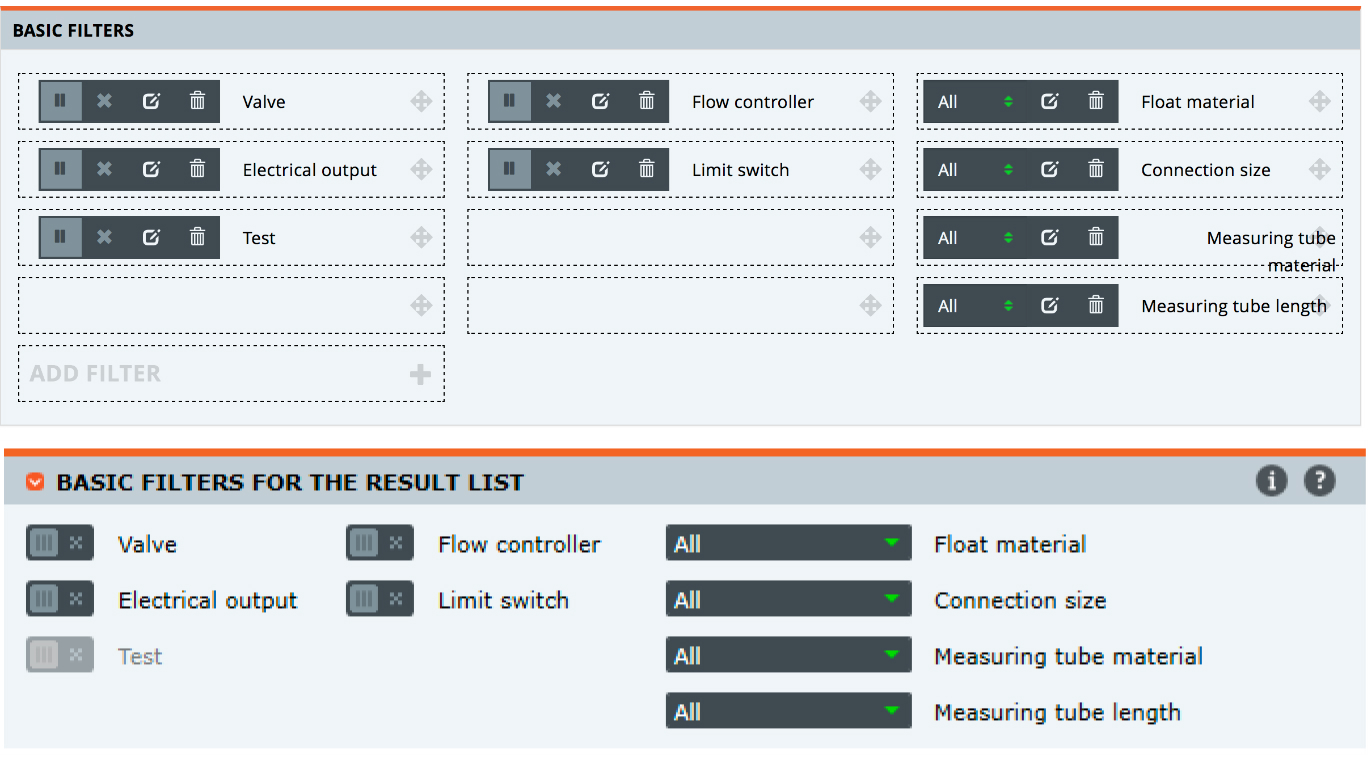
\includegraphics[width=1.0\textwidth]{testergebnis} %{CS0031}
\caption{Vergleich der Webanwendung und FlowConfigurator Software nach dem durchgeführten Integrationstest}
\label{fig:test}
\end{figure}

Auf dem Vergleichsbild lässt sich erkennen, dass der neu angelegte Testfilter, sowohl in der Webanwendung, als auch in der FlowConfigurator Software an der richtigen Stelle angezeigt wird. Auch wenn das entwickelte Testszenario formal alle aufgestellten funktionalen Anforderungen abdeckt und alle erwarteten Ergebnisse bestätigt werden konnten, kann das angewandte Testverfahren nur grob eine Aussage über die tatsächliche Funktionsfähigkeit der Webanwendung geben. Bei dem angewandten Testszenario handelt es sich zwar um die typische angedachte Benutzungsweise der Webanwendung, es wurden allerdings keine Randbedingungen untersucht. Abschließend lässt sich dennoch, auf Grundlage des durchgeführten Tests, die Behauptungen aufstellen, das mit dem entwickelten Prototypen, die am Anfang der Arbeit definierte Zielsetzung erreicht werden konnte.
\chapter{Ergebnis}
\label{cha:Ergebnis}
Als Abschluss der vorliegenden Arbeit wird in diesem Kapitel auf die erreichten Ziele eingegangen, sowie ein Ausblick für mögliche Verbesserungen gegeben.

Das Ziel der Arbeit war, eine Webanwendung zu entwickeln mit der es möglich ist komplexe Filterdaten, im Kontext der von der netbase GmbH entwickelten FlowConfigurator Software, zu verwalten. Zu diesem Zweck wurden die bestehende Softwarelösung und die Datenbasis analysiert und daraus Anforderungen an die Webanwendung abgeleitet. Darauf aufbauend erfolgte ein Systementwurf, in dem mit Hilfe von Diagrammen die Anwendung modelliert und dargestellt wurde. Ein Schwerpunkt dieses Entwurfs war die Gestaltung der Benutzeroberfläche auf Grundlage von WYSIWYG-Prinzipien. Anschließend wurde der Systementwurf implementiert und dessen Umsetzung anhand von Quellcodebeispielen erläutert. Abschließend wurde anhand einer vorgestellten Testmethode die Funktionsfähigkeit des entwickelten Prototypen untersucht.

\section{Bewertung}

Anhand von Vorbetrachtungen und Analysen der Funktionsweise der FlowConfigurator Software auf Grundlage einer bestehenden Datenbasis, konnte gezeigt werden, wie sich bereits bestehende Prozesse bei der Verarbeitung komplexer Datenstrukturen als Ausgangspunkt für die Entwicklung einer Datenpflegeanwendung nutzen lassen. Die aus der Analyse der Datenstruktur und der Betrachtung der Benutzeroberfläche der FlowConfigurator Software gewonnenen Erkenntnisse konnten abstrahiert als Teile eines Systementwurfs verwendet werden. Der entworfene Prototyp ist in seiner Anwendung sehr flexibel gestaltet worden. Die starke Trennung der Systemkomponenten und die Realisierung eines vielseitig ansprechbaren REST konformen Webservice ermöglichen es, die Anwendung mit geringem Aufwand weiter zu entwickeln und zu modifizieren. Die Benutzeroberfläche konnte nahe am Vorbild der FlowConfigurator Software konzipiert werden, ohne dabei auf Vorteile einer webgestützten Anwendung verzichten zu müssen. Die dabei verwendeten WYSIWYG-Konzepte für die Anpassung von Filtersteuerelementen fügen sich dank modernen und interaktiven Drag-and-Drop Mechanismen nahtlos in den Bearbeitungsvorgang der Filterdaten ein. Die direkte Manipulation von Filtersteuerelementen sind dabei eine sinnvolle Ergänzung zu der ebenfalls implementierten und auf Dateneingabemasken gestützten Bearbeitung der Filterdaten. Die in Abschnitt \ref{sec:Funktionale Anforderungen} erarbeiteten funktionalen Anforderungen konnten vollständig implementiert werden. Ausnahme ist hier die Anforderung \emph{Models hinzufügen}, die aus zeitlichen Gründen nicht erfolgen konnte, von dem Systementwurf aber abgedeckt wird. Außerdem bestehen Probleme bei der datengetriebenen Generierung der Filtersteuerelemente in der Webanwendung. Diese Probleme begründen sich im angewandten Grid-System zur Platzierung der Filtersteuerelemente, da die Datenbasis auf ein Fließlayout ausgerichtet ist. Die an die Anwendung gestellten Tests konnten aus diesem Grund nur mit Einschränkung bestanden werden. Der Systementwurf und die Implementierung demonstrieren dennoch, wie die Pflege komplexer Datenstrukturen unter Anwendung von interaktiven Bearbeitungskonzepten auf Grundlage des WYSIWYG-Prinzips umgesetzt werden kann.

\section{Ausblick}

Im Folgenden werden Themen genannt, anhand derer sich der Prototyp erweitern oder verbessern lässt.

Aufgrund komplexer Datenabfragen und nicht optimierter Algorithmen beim Zugriff auf die entwickelte Schnittstelle kommt es in der Webanwendung gelegentlich zu erhöhten Ladezeiten. Durch eine Identifizierung der Schwachstellen kann die Performance des Webservice noch erheblich optimiert werden, um eine reibungslose Bearbeitung der Filterdaten in der Webanwendung zu fördern. Weiterhin weist der entwickelte Algorithmus, für die Konvertierung der layoutspezifischen Filterdaten von einem Fließlayout hin zu einem Grid-Layout Schwachstellen auf. Der Algorithmus basiert bereits auf einem generischen Ansatz, der aufgrund der Komplexität der zugrunde liegenden Daten, aber noch nicht mit allen auftretenden Randbedingungen umgehen kann. Außerdem wurde serverseitig nur eine prototypische Implementierung für die Validierung der zu persistierenden Daten realisiert. Um schwere Ausnahmefehler auf Datenbankebene zu verhindern und ein besseres Fehlerverhalten zu gewährleisten ist es notwendig, Fehler frühzeitig abzufangen und aussagekräftige Fehlermeldungen zu generieren. Insgesamt ist damit festzustellen, dass das Potential der entwickelten Anwendung noch nicht ausgeschöpft ist und in seiner prototypischen Realisierung viel Raum für Erweiterungsmöglichkeiten vorhanden ist.

%%%----------------------------------------------------------
\appendix                                            % Anhang 
%%%----------------------------------------------------------

%\include{back/anhang_a}	% Technische Ergänzungen
%\include{back/anhang_b}	% Inhalt der CD-ROM/DVD
%\include{back/anhang_c}	% Chronologische Liste der Änderungen
%\include{back/anhang_d}	% Quelltext dieses Dokuments

%%%----------------------------------------------------------
\MakeBibliography                        % Quellenverzeichnis
%%%----------------------------------------------------------

%%% Erkärung------------------------------
\begin{german}
\chapter*{Erkl\"arung}
\noindent
%Standardfassung der FH-OOe ab 04.04.2012:
Ich erkl\"are eidesstattlich, dass ich die vorliegende Arbeit selbstst\"andig und ohne fremde Hilfe verfasst, 
andere als die angegebenen Quellen nicht benutzt und die den benutzten Quellen entnommenen Stellen als 
solche gekennzeichnet habe. Die Arbeit wurde bisher in gleicher oder \"ahnlicher Form keiner anderen 
Pr\"ufungsbeh\"orde vorgelegt.
\par
\vspace{10mm}
\noindent
Berlin, am 5. September 2016
\par
\vspace{12mm}
\noindent
Benjamin Schuch
\end{german}
%%%----------------------------------------------------------

%%% Messbox zur Druckkontrolle ------------------------------
%%%\chapter*{Messbox zur Druckkontrolle}



\begin{center}
{\Large --- Druckgröße kontrollieren! ---}

\bigskip

\Messbox{100}{50} % Angabe der Breite/Hoehe in mm

\bigskip

{\Large --- Diese Seite nach dem Druck entfernen! ---}

\end{center}



%%%----------------------------------------------------------
\end{document}
%%%----------------------------------------------------------